% Options for packages loaded elsewhere
\PassOptionsToPackage{unicode}{hyperref}
\PassOptionsToPackage{hyphens}{url}
%
\documentclass[
  12pt,
]{article}
\usepackage{subcaption}
\usepackage{comment}
\usepackage{graphicx}
\usepackage{amsmath,amssymb}
\usepackage{lmodern}
\usepackage{iftex}
\ifPDFTeX
  \usepackage[T1]{fontenc}
  \usepackage[utf8]{inputenc}
  \usepackage{textcomp} % provide euro and other symbols
\else % if luatex or xetex
  \usepackage{unicode-math}
  \defaultfontfeatures{Scale=MatchLowercase}
  \defaultfontfeatures[\rmfamily]{Ligatures=TeX,Scale=1}
\fi
% Use upquote if available, for straight quotes in verbatim environments
\IfFileExists{upquote.sty}{\usepackage{upquote}}{}
\IfFileExists{microtype.sty}{% use microtype if available
  \usepackage[]{microtype}
  \UseMicrotypeSet[protrusion]{basicmath} % disable protrusion for tt fonts
}{}
\makeatletter
\@ifundefined{KOMAClassName}{% if non-KOMA class
  \IfFileExists{parskip.sty}{%
    \usepackage{parskip}
  }{% else
    \setlength{\parindent}{0pt}
    \setlength{\parskip}{6pt plus 2pt minus 1pt}}
}{% if KOMA class
  \KOMAoptions{parskip=half}}
\makeatother
\usepackage{xcolor}
\usepackage[margin=1in]{geometry}
\usepackage{graphicx}
\makeatletter
\def\maxwidth{\ifdim\Gin@nat@width>\linewidth\linewidth\else\Gin@nat@width\fi}
\def\maxheight{\ifdim\Gin@nat@height>\textheight\textheight\else\Gin@nat@height\fi}
\makeatother
% Scale images if necessary, so that they will not overflow the page
% margins by default, and it is still possible to overwrite the defaults
% using explicit options in \includegraphics[width, height, ...]{}
\setkeys{Gin}{width=\maxwidth,height=\maxheight,keepaspectratio}
% Set default figure placement to htbp
\makeatletter
\def\fps@figure{htbp}
\makeatother
\setlength{\emergencystretch}{3em} % prevent overfull lines
\providecommand{\tightlist}{%
  \setlength{\itemsep}{0pt}\setlength{\parskip}{0pt}}
\setcounter{secnumdepth}{5}
\newlength{\cslhangindent}
\setlength{\cslhangindent}{1.5em}
\newlength{\csllabelwidth}
\setlength{\csllabelwidth}{3em}
\newlength{\cslentryspacingunit} % times entry-spacing
\setlength{\cslentryspacingunit}{\parskip}
\newenvironment{CSLReferences}[2] % #1 hanging-ident, #2 entry spacing
 {% don't indent paragraphs
  \setlength{\parindent}{0pt}
  % turn on hanging indent if param 1 is 1
  \ifodd #1
  \let\oldpar\par
  \def\par{\hangindent=\cslhangindent\oldpar}
  \fi
  % set entry spacing
  \setlength{\parskip}{#2\cslentryspacingunit}
 }%
 {}
\usepackage{calc}
\newcommand{\CSLBlock}[1]{#1\hfill\break}
\newcommand{\CSLLeftMargin}[1]{\parbox[t]{\csllabelwidth}{#1}}
\newcommand{\CSLRightInline}[1]{\parbox[t]{\linewidth - \csllabelwidth}{#1}\break}
\newcommand{\CSLIndent}[1]{\hspace{\cslhangindent}#1}
\usepackage{float}
\usepackage{amsmath}
\usepackage{graphicx}
\usepackage{nicefrac}
\usepackage{setspace}
\doublespacing
\let\rfb\reflectbox
\usepackage{geometry}
\geometry{left=1in,right=1in,top=1in,bottom=1in}
\usepackage{indentfirst}
\setlength{\parindent}{2em}   % <-- paragraph indent
\setlength{\parskip}{0pt}     % <-- no extra spacing
\usepackage{booktabs}
\usepackage{graphicx}
\usepackage{longtable}
\usepackage{array}
\usepackage{multirow}
\usepackage{wrapfig}
\usepackage{float}
\usepackage{colortbl}
\usepackage{pdflscape}
\usepackage{tabu}
\usepackage{threeparttable}
\usepackage{threeparttablex}
\usepackage[normalem]{ulem}
\usepackage{makecell}
\usepackage{xcolor}
\ifLuaTeX
  \usepackage{selnolig}  % disable illegal ligatures
\fi
\IfFileExists{bookmark.sty}{\usepackage{bookmark}}{\usepackage{hyperref}}
\IfFileExists{xurl.sty}{\usepackage{xurl}}{} % add URL line breaks if available
\urlstyle{same} % disable monospaced font for URLs
\hypersetup{
  pdftitle={Plan B: E-MS},
  pdfauthor={Brandon Payne},
  hidelinks,
  pdfcreator={LaTeX via pandoc}}

%Exploring the operationg characteristics of the EMS on QTL data
%Comparisons of Expectation-Maximization-Model Selection
\title{Plan B: Operating Characteristics of Expectation-Maximization Model Selection for QTL Mapping}
\usepackage{etoolbox}
\makeatletter
\providecommand{\subtitle}[1]{% add subtitle to \maketitle
  \apptocmd{\@title}{\par {\large #1 \par}}{}{}
}
\makeatother
\subtitle{A THESIS SUBMITTED IN PARTIAL FULFILLMENT OF THE REQUIREMENTS
FOR THE DEGREE OF MASTER OF PUBLIC HEALTH DATA SCIENCE

Committee:

Dr.~J. Sunil Rao (Plan B Advisor) 

Dr.~Lynn Eberly (Academic
Advisor) 

Dr.~Weihong Tang}
\author{Brandon Payne}
\date{April 28, 2026}

\begin{document}
\maketitle

\newpage

\hypertarget{abstract}{%
\section*{Abstract}\label{abstract}}
\addcontentsline{toc}{section}{Abstract}

Missing data remains a persistent challenge across fields such as
genetics, epidemiology, and social sciences. One critical yet
under-addressed issue in the treatment of incomplete data is double
dipping, the inappropriate reuse of data in both model selection and
inference (\protect\hyperlink{ref-Sunilems}{Jiang, Nguyen, and Rao
2015}, \protect\hyperlink{ref-jiang2011best}{2011}). This work
investigates how double dipping manifests in the context of missing data
imputation and demonstrates that the Expectation-Maximization-Model
Selection (E-MS) framework (\protect\hyperlink{ref-Sunilems}{Jiang,
Nguyen, and Rao 2015}) effectively addresses aspects of this problem.
We compare E-MS to conventional methods across a range of
data-generating scenarios under different missing data mechanisms,
including missing completely at random (MCAR), missing at random (MAR),
and missing not at random (MNAR). Large-scale simulations are conducted
to assess the robustness of E-MS and to evaluate its performance
relative to existing approaches. Results demonstrate that E-MS mitigates
key biases associated with double dipping, consistently outperforming
conventional methods by achieving superior F1 scores through high recall
coupled with strong precision.

\section{Introduction}

In applied statistical analysis, missing data is an unavoidable and
often complex obstacle. Whether due to non-response in surveys, sensor
failure in experiments, or limitations in sequencing technologies in
genomics, analysts must frequently address datasets with incomplete
observations. The implications of improper handling of missingness are
far-reaching, especially when decisions about model structure or
inference procedures are based on incomplete information.

This paper focuses on a particular consequence of missing data analysis:
double dipping (\protect\hyperlink{ref-Sunilems}{Jiang, Nguyen, and Rao
2015}, \protect\hyperlink{ref-jiang2011best}{2011}). This occurs when
the same data is used in multiple stages of model development without
proper adjustment, typically in both model selection and inference. Such
practices can inflate Type I error rates and lead to misleading
conclusions. The goal of this work is to understand how imputation
methods, particularly the E-MS algorithm, interact with and potentially
exacerbate or alleviate double dipping.

Prior work has shown that standard information criteria applied directly
to incomplete logistic regression data can systematically favor
underspecified models. For example,
(\protect\hyperlink{ref-IbrahimZhuTang2008}{Ibrahim, Zhu, and Tang
2008}) demonstrate that, under a missing at random mechanism, the
intercept-only model may maximize the conditional expected
log-likelihood even when it is not the true model. This phenomenon can
lead traditional Bayesian Information Criterion (BIC)-based selection procedures, such as the BIC penalty
denoted by IZT, to consistently choose an incorrect model. Through
simulations across different sample sizes, true model structures, and
both ignorable and nonignorable missingness mechanisms, they show that
alternative methods like E-MS achieve substantially higher true positive
rates and are more robust to the missingness mechanism
(\protect\hyperlink{ref-IbrahimZhuTang2008}{Ibrahim, Zhu, and Tang
2008}; \protect\hyperlink{ref-rubin1976inference}{Rubin 1976}).

\section{Missing Data}

To understand the challenges of missing data, we must first establish
notation. Let $Y = (Y_{\text{o}}, Y_{\text{m}})$
denote the complete data matrix, where $Y_{\text{o}}$ represents
the observed values and $Y_{\text{m}}$ the missing values. Define
the missingness indicator $R_i \in \{0,1\}$, where $R_i = 1$ if observation
$i$ is observed and $R_i = 0$ if it is missing, with parameter
$\phi$ governing the missingness mechanism and $\theta$
governing the data-generating process. The joint distribution then factorizes as:
\[
P(Y, R \mid \theta, \phi) =
P(Y \mid \theta) \cdot
P(R \mid Y, \phi)
\]
The three missing data mechanisms, introduced by
\protect\hyperlink{ref-rubin1976inference}{Rubin (1976)},
are distinguished by the structure of
$P(R \mid Y, \phi)$
and form a strict hierarchy: MCAR $\subset$ MAR $\subset$ MNAR.

Missing at Random (MAR) refers to a situation where the probability of
missing data depends only on the observed data and not on the unobserved
(missing) data. Formally:
\[
P(R \mid Y, \phi) =
P(R \mid Y_{\text{o}}, \phi)
\]
In other words, once we account for the observed variables, any remaining
missingness is random with respect to the missing values themselves. This
allows for unbiased estimation if the missingness is properly accounted for
in the analysis. On the other hand, Missing Not at Random (MNAR) occurs when
the probability of missing data depends on the unobserved data itself, even
after accounting for the observed data:
\[
P(R \mid Y, \phi) =
P(R \mid Y_{\text{o}}, Y_{\text{m}},
\phi)
\]
where the dependence on $Y_{\text{m}}$ cannot be reduced to a
function of $Y_{\text{o}}$ alone. This introduces potential bias
because the missingness is directly related to the values of the missing
data, making it more challenging to handle in statistical analyses without
making strong assumptions about the missing data mechanism. Understanding
whether data are MAR or MNAR is crucial for applying appropriate statistical
methods and drawing valid conclusions from incomplete datasets.

While Missing Completely at Random (MCAR) would be a special case where
missingness is entirely independent of both observed and unobserved data:
\[
P(R \mid Y, \phi) = P(R \mid
\phi), \quad \text{i.e.,} \quad
R \perp\!\!\!\perp Y
\]
this assumption is rarely met in real-world data. The three mechanisms are
therefore nested, with MCAR being the most restrictive special case and MNAR
the most general:
\[
\text{MCAR} \implies \text{MAR} \implies \text{MNAR}
\]

Incomplete cases, particularly those with only 20--40\% of the full
information available, often appear in genetic studies such as
Quantitative Trait Loci (QTL) mapping, where limitations in data collection
or sequencing coverage lead to substantial gaps. While several approaches
exist to handle such missing data, ranging from complete-case analysis to multiple
imputation, few adequately address the implications of using imputed data
during both model selection and final inference.

\section{Imputation}

Single imputation methods replace each missing value with one
deterministic estimate. Although these approaches are easy to implement
and computationally efficient, they often fail to capture the
uncertainty inherent in missing data. One of the most widely used
approaches is mean, median, or mode imputation, in which a missing value
is replaced with a measure of central tendency derived from the observed
data. While this method preserves sample size and is straightforward to
apply, it artificially reduces variability and can bias parameter
estimates, especially when the data are not missing completely at random
(\protect\hyperlink{ref-little2002statistical}{Little and Rubin 2002}).

Another form of single imputation is regression imputation, where
missing values are predicted using a regression model built from the
observed cases. Although regression-based approaches provide more
plausible values than simple mean imputation, they still tend to
overstate the precision of the data by treating predicted values as
known quantities (\protect\hyperlink{ref-Allison2011}{Allison 2011}).

Multiple imputation, introduced by
(\protect\hyperlink{ref-rubin1987multiple}{Rubin 1987}), is widely
considered the gold standard for handling missing data in many applied
research contexts. Instead of substituting missing values with a single
estimate, MI generates multiple versions of the dataset, each containing
different plausible imputations drawn from a predictive distribution
that reflects both observed data and uncertainty.

After statistical analyses are performed separately on each imputed
dataset, the results are combined using Rubin's rules, which account for
both within-imputation and between-imputation variability. This leads to
unbiased parameter estimates and valid standard errors when data are
missing at random (MAR) 
(\protect\hyperlink{ref-vanBuuren2018}{Van Buuren 2018}). Although MI requires more
computation and careful model specification than single imputation, its
ability to incorporate uncertainty makes it far more statistically
robust.

Model-based imputation methods leverage statistical or machine learning
models to estimate missing values in a data-driven manner. These
approaches are often more flexible than traditional single or multiple
imputation.

A foundational model-based method is the Expectation--Maximization (EM)
algorithm, which iteratively estimates missing data by maximizing the
likelihood of the observed data under assumed model parameters
(\protect\hyperlink{ref-dempster1977maximum}{Dempster, Laird, and Rubin
1977}). EM produces maximum likelihood estimates but does not generate
multiple datasets, so it does not account for imputation uncertainty
unless paired with MI.

Machine-learning--oriented methods have become increasingly popular.
k-Nearest Neighbors (kNN) imputation identifies cases with similar
feature profiles and uses their observed values to fill in missing
entries. Random forest--based methods, such as missForest, build
ensembles of decision trees to predict missing values; they can handle
nonlinear relationships and mixed data types effectively
(\protect\hyperlink{ref-Stekhoven2012}{Stekhoven and Bühlmann 2012}).
More recently, deep learning autoencoder imputation has been used to
reconstruct missing values by learning compressed representations of the
full dataset, making it particularly effective in high-dimensional or
complex data structures.

Model-based imputation techniques offer strong predictive performance
and flexibility, especially in modern large-scale datasets. However,
they require careful tuning and may not inherently provide valid
measures of uncertainty unless extended within a multiple-imputation
framework.

\section{Double Dipping Problem}

In high-dimensional QTL studies and related genetic mapping contexts, a common analytical workflow uses the same dataset both to select models and to estimate their parameters or significance. This practice, often referred to as double dipping or circular analysis, arises when data are used first to generate hypotheses or select features and then reused to estimate or test those features without accounting for the selection process. The statistical danger of this workflow has been well documented in other fields, particularly in neuroimaging, where it was shown that re-analyzing data after selection leads to systematically biased effect sizes and invalid inferential statements (Kriegeskorte et al. (\protect\hyperlink{ref-Kriegeskorte2009}{2009})). QTL mapping is a particularly acute instance of this problem. Because the number of candidate loci vastly exceeds the number of observations, researchers must scan across the genome and select regions that exceed some significance threshold — yet most classical statistical inference assumes that the model was specified independently of the data used to estimate it. In QTL mapping, this assumption is routinely violated and the impact is magnified by the scale, sparsity, and missingness that characterize such data.

Markers, covariates, and interaction structures are typically chosen
using data-dependent criteria such as likelihood scans, penalized
regression, or information criteria, and the same data are then used to
estimate effect sizes and uncertainties for the selected loci.
Conditioning on the outcome in this way induces selection bias: the
chosen loci are those that happened to align with random fluctuations,
imputation artifacts, or sampling noise, and treating the selected model
as fixed ignores this conditioning. As a result, estimated genetic
effects are biased away from zero and uncertainty is understated, even
when model selection is performed using principled criteria rather than
hypothesis testing (Pasaniuc and Price
(\protect\hyperlink{ref-Pasaniuc2017}{2017})).

This issue becomes more severe in the presence of missing data and
genotype imputation, which are now unavoidable in modern QTL studies.
High-resolution mapping pipelines rely on probabilistic reconstruction
of unobserved genotypes from low-coverage sequencing or from related
individuals, often in complex multi-parent populations (Huang et al.
(\protect\hyperlink{ref-Huang2012}{2012}); Karl W. Broman et al.
(\protect\hyperlink{ref-Broman2017}{2017})). These imputation models are
trained on the observed data and encode assumptions about haplotype
structure, recombination, and linkage disequilibrium. When the imputed
values are then treated as fixed inputs to downstream QTL scans, the
uncertainty and model dependence introduced during imputation are
effectively ignored. If marker selection or model fitting is carried out
on these imputed datasets, the selection step itself is influenced by
the imputation model, which further entangles model choice with the
observed data and amplifies double-dipping bias. In this sense,
sophisticated imputation does not remove the inferential problem; it
relocates it into a more complex, and often hidden, modeling layer.

The practical response to multiple testing in QTL studies is rarely to
rely on strict p-value thresholds alone, because the number of candidate
loci is enormous and effect sizes are typically small. Instead,
researchers often adopt penalized likelihoods, Bayesian model
probabilities, or criteria such as BIC to balance goodness-of-fit
against model complexity. While these tools are well suited for
high-dimensional search, they do not by themselves resolve the
inferential consequences of data-dependent model choice. Once a model is
selected, standard errors, posterior summaries, or test statistics are
usually computed as if the model were fixed in advance, even though it
was chosen precisely because it fit the data unusually well. This
creates a false sense of certainty about the importance of specific
loci, and it is one of the main drivers of the winner's-curse and
reproducibility problems in genetic association studies.

A concrete illustration of how information criteria can fail under
missing data and data-dependent model selection is given by the
following example 
\protect\hyperlink{ref-IbrahimZhuTang2008}{(Ibrahim, Zhu, and Tang
2008)}.

Suppose that one attempts to select a logistic model,
$\text{logit}(\pi_i) = \mathbf{x}_i^\top \boldsymbol{\beta}$, where
$\pi_i = P(Y_i = 1)$, $Y_1, \ldots, Y_n$ being independent binary
observations and $\mathbf{x}_i$ is a vector of covariates to be
selected. Suppose that $y_1, \ldots, y_5$ are observed and the rest of
the $y_i$'s are missing. For simplicity, assume that all the
$\mathbf{x}_i$'s are observed and that missingness is MAR \protect\hyperlink{ref-rubin1976inference}{(Rubin 1976)} for simplicity.

Let $M_0$ denote the intercept-only model and suppose that the true
model is not $M_0$. The complete-data log-likelihood under $M_0$ is $\ell = \sum_{i=1}^{n}   \bigl\{y_i \log p_0 + (1 - y_i)\log(1 - p_0)\bigr\},$
where $p_0 = e^{\beta_0}/(1 + e^{\beta_0})$ and $\beta_0$ is the
intercept. Under $M_0$ the conditional expectation given the observed
data is $E\!\left(\ell \mid y_1, \ldots, y_5,\, \text{all } \mathbf{x}_i\right) =  \sum_{i=1}^{5}  \bigl\{y_i \log p_0 + (1 - y_i)\log(1 - p_0)\bigr\} + (n-5)\bigl\{p_0 \log p_0 + (1-p_0)\log(1-p_0)\bigr\}.$
If $y_i = 1$ for $1 \le i \le 5$, then as $p_0 \to 1$ the expression
above tends to $0$.
On the other hand, under any competing model $M$ the corresponding
log-likelihood satisfies
$\ell = \sum_{i=1}^{n}\{y_i \log p_i + (1-y_i)\log(1-p_i)\} \le 0$,
so $E(\ell \mid y_1, \ldots, y_5, \text{all } \mathbf{x}_i) \le 0$
under $M$.

Therefore the maximized conditional expectation of $\ell$ under $M_0$
(which is $0$) is greater than or equal to that under any $M$. Because
$M_0$ also has the smallest dimension, every information criterion of
the form considered by \protect\hyperlink{ref-IbrahimZhuTang2008}{(Ibrahim, Zhu, and Tang
2008)} will select $M_0$, the
intercept-only model, even though it is known to be incorrect. This
shows that principled information criteria can still systematically
favor the wrong model whenever missing data create a degenerate
likelihood surface for the simplest candidate.

Recent methodological surveys in high-dimensional biomedical inference
emphasize that many modern pipelines successfully address feature
selection, prediction, and missingness, yet still leave unresolved the
deeper statistical issue of how to perform valid inference after
selection (Serghiou et al.
(\protect\hyperlink{ref-Serghiou2023}{2023})). In QTL mapping, where
model search, imputation, and inference are tightly interwoven, this gap
is particularly consequential. Double dipping is therefore not a
technical detail about p-values versus information criteria; it is a
structural problem that arises whenever the same data are used to decide
what model to believe and to quantify how strongly that model is
supported. Without accounting for this dependency, QTL analyses can
produce inflated effect estimates, underestimated uncertainty, and
spurious discoveries, even when every individual modeling step appears
statistically sound.

\section{Existing Approaches}

\begin{comment} %lasso wasn't used in the paper
\subsection{LASSO}

The Least Absolute Shrinkage and Selection Operator (Lasso), introduced
by (\protect\hyperlink{ref-tibshirani1996regression}{Tibshirani 1996}),
is a regularization-based regression method designed for settings where
model interpretability and prediction accuracy are both important,
particularly in high-dimensional regimes where the number of predictors
\(p\) may be comparable to or larger than the sample size \(n\). Lasso
extends ordinary least squares by adding an \(\ell_1\) penalty on the
regression coefficients, which encourages sparsity and enables
simultaneous variable selection and estimation.

Formally, suppose the data follow the linear regression model \[
y = X\beta + \varepsilon,
\] where \(y \in \mathbb{R}^n\) denotes the response vector,
\(X \in \mathbb{R}^{n \times p}\) is the design matrix of predictors,
\(\beta \in \mathbb{R}^p\) is the vector of unknown regression
coefficients, and \(\varepsilon\) represents random error. The Lasso
estimator is obtained by solving the penalized least-squares problem
\begin{equation*}
\hat{\beta}^{\text{lasso}}
= \arg\min_{\beta}
\left\{
\frac{1}{2n}\|y - X\beta\|_2^2
+ \lambda \|\beta\|_1
\right\}
\end{equation*} where \(|\beta|1 = \sum{j=1}^p |\beta_j|\) denotes the
\(\ell_1\) norm and \(\lambda \ge 0\) is a tuning parameter that
controls the degree of regularization. Larger values of \(\lambda\)
impose stronger shrinkage, forcing more coefficients to be exactly zero
and producing a sparse model that retains only the most relevant
predictors.

This sparsity-inducing property makes Lasso particularly appealing for
imputation and prediction tasks in complex data environments. When
imputing missing values, Lasso can identify a small set of informative
predictors that contribute most strongly to the conditional expectation
of the missing variable, thereby reducing variance and mitigating
overfitting. More broadly, Lasso is widely used in genomics, finance,
and machine learning for handling multicollinearity, improving
prediction accuracy, and producing interpretable models in
high-dimensional settings.

Despite these advantages, standard Lasso formulations struggle in the
presence of missing data. Classical Lasso assumes that both the response
vector \(y\) and the design matrix \(X\) are fully observed. In
practice, widely used implementations require complete data matrices,
and will either fail or implicitly discard observations containing
missing values. Unlike certain tree-based or ensemble methods, Lasso
does not natively incorporate mechanisms for handling missingness during
model fitting.

As a consequence, the quality of any preprocessing step becomes
critical. If missing values are imputed poorly before applying Lasso,
the resulting coefficient estimates and variable selection can be
severely biased. Since the \(\ell_1\) penalty is sensitive to the scale
and structure of the predictors, errors introduced during imputation may
lead to incorrect exclusion of relevant variables or inclusion of
spurious ones.

Several workarounds are commonly employed in practice. The most
straightforward approach is to apply an imputation procedure prior to
fitting the Lasso model, using methods such as mean imputation,
\(k\)-nearest neighbors, or more sophisticated approaches like multiple
imputation by chained equations
(\protect\hyperlink{ref-vanBuuren2011MICE}{Buuren and
Groothuis-Oudshoorn 2011}). Alternatively, research has proposed
modified versions of Lasso that explicitly account for missing data,
including EM-based Lasso formulations or joint models that combine
imputation and coefficient estimation within a unified framework. While
these extensions offer theoretical improvements, they are not yet
standard in most applied software.

\end{comment}

\subsection{QTL}

Quantitative trait locus (QTL) mapping seeks to identify genomic regions
that are associated with variation in a quantitative phenotype. In
practice, QTL analysis must account for missing or unobserved genotype
information between genetic markers, which arises naturally due to
limited marker density. The \texttt{R/qtl} framework, as developed and
documented by (\protect\hyperlink{ref-Broman2019}{Karl W. Broman et al.
2019}) and the \texttt{rqtl} manual, provides a comprehensive set of
tools for addressing this problem using likelihood- and regression-based
approaches.

To identify markers of interest, QTL mapping is commonly performed using
three complementary methods: expectation--maximization (EM) algorithms
(\protect\hyperlink{ref-dempster1977maximum}{Dempster, Laird, and Rubin
1977}; \protect\hyperlink{ref-lander1989mapping}{Lander and Botstein
1989}), Haley--Knott (HK) regression
(\protect\hyperlink{ref-haley1992simple}{Haley and Knott 1992}), and
multiple imputation approaches
(\protect\hyperlink{ref-sugiyama2001concordance}{Sugiyama et al. 2001}).
All three methods rely on the same underlying genetic model but differ
in how they handle uncertainty in the unobserved genotypes at putative
QTL positions.

The EM-based approach treats the underlying QTL genotypes as latent
variables. At each genomic position, the E-step computes the conditional
probabilities of the possible QTL genotypes given the observed marker
data and current parameter estimates, while the M-step maximizes the
expected complete-data log-likelihood to update model parameters. This
method provides statistically efficient inference but can be
computationally intensive, particularly for large genomes or complex
crosses.

Haley--Knott regression offers a computationally simpler approximation
to the EM algorithm. Instead of fully iterating between expectation and
maximization, HK regression replaces the unobserved QTL genotypes with
their conditional expectations and fits a standard linear regression
model. While this approximation leads to substantial gains in speed, it
may result in a modest loss of efficiency compared to the full EM
approach, especially in regions with sparse marker information.

Multiple imputation methods take a different perspective by repeatedly
sampling complete genotype datasets from the conditional distribution of
the missing genotypes given the observed markers. For each imputed
dataset, a standard QTL scan is performed, and the results are combined
across imputations. This strategy more fully propagates uncertainty in
the missing genotypes and often yields more robust inference, at the
cost of increased computational effort.

In genomic applications, QTL mapping is typically conducted on
large-scale datasets involving thousands of genetic markers and, in
modern studies, potentially thousands of individuals. In such settings,
even small systematic errors in the handling or imputation of missing
genotype data can accumulate and substantially bias downstream
inference \protect\hyperlink{ref-Fan2008}{(Fan 2008)}.  Poorly specified imputation models may distort conditional
genotype probabilities, inflate or attenuate LOD scores, and lead to
spurious QTL detection or missed true signals. Consequently, careful
treatment of missing data is critical, as incorrect imputation can
greatly skew results despite large sample sizes that might otherwise
suggest statistical robustness.

For each mapping method, a genome-wide scan yields a profile of
logarithm of the odds (LOD) scores that measure the strength of evidence
for the presence of a QTL at each genomic position. Statistical
significance is assessed by applying a predefined LOD threshold to these
scan results, and all genomic locations where the LOD score exceeds this
threshold are identified as candidate QTL. Reporting all detected peaks
across the genome for each method enables a systematic comparison of the
number, location, and strength of QTL signals, facilitating evaluation
of detection consistency and relative mapping performance among the EM,
Haley--Knott, and multiple imputation approaches.

\subsection{EM - The Expectation-Maximization}

The Expectation--Maximization (EM) algorithm, introduced by
(\protect\hyperlink{ref-dempster1977maximum}{Dempster, Laird, and Rubin
1977}), provides a likelihood-based framework for parameter estimation
in the presence of missing or latent data. Its appeal lies in its
conceptual simplicity and broad applicability across a wide range of
statistical models. Let \(Y_o\) denote the observed data, \(Y_m\) the
missing or latent data, and \(\theta\) the vector of unknown parameters.
If the complete data \(Y = (Y_o, Y_m)\) were fully observed, inference
would proceed by maximizing the complete-data log-likelihood
\(\ell_c(\theta) = \log p(Y_o, Y_m \mid \theta)\). Because \(Y_m\) is
unobserved, direct maximization of the observed-data likelihood
\(\ell(\theta) = \log p(Y_o \mid \theta)\) is often analytically
intractable. EM addresses this difficulty by iteratively maximizing a
surrogate objective function that is easier to handle.

At iteration \(t\), the E-step constructs the function \[
Q(\theta \mid \theta^{(t)})
= \mathbb{E}_{Y_m \mid Y_o, \theta^{(t)}}
\big[ \log p(Y_o, Y_m \mid \theta) \big],
\] which is the conditional expectation of the complete-data
log-likelihood with respect to the distribution of the missing data
given the observed data and the current parameter estimates
\(\theta^{(t)}\). This step does not impute missing values
deterministically; instead, it averages over their conditional
distribution under the current model, thereby producing an expected
log-likelihood that reflects the uncertainty induced by missingness, but
only through expectation rather than full probabilistic propagation.

The M-step then updates the parameter estimates by maximizing this
expected log-likelihood, \[
\theta^{(t+1)} = \arg\max_{\theta} Q(\theta \mid \theta^{(t)}).
\] This optimization yields new parameter values that increase, or at
least do not decrease, the observed-data likelihood. Repeating the
E-step and M-step generates a sequence \({\theta^{(t)}}\) with the
property that \(\ell(\theta^{(t+1)}) \ge \ell(\theta^{(t)})\), and the
algorithm is guaranteed to converge to a stationary point of the
likelihood under mild regularity conditions.

Despite its strengths, EM has several important limitations. First, it
assumes that the model specified for the complete data is correct; any
model misspecification directly affects both the conditional
distribution used in the E-step and the optimization performed in the
M-step. Second, although the E-step computes expectations over the
missing data, EM ultimately treats these expectations as fixed
quantities in the M-step, and therefore does not fully propagate
uncertainty in the latent variables into parameter uncertainty. Third,
the likelihood surface in models with latent structure is often
multimodal, and EM may converge to a local rather than global maximum
depending on initialization.

\section{E-MS}

The E--M algorithm is well known for parameter estimation in the presence of
missing data. On the other hand, model selection, as another component
of model identification, may also be viewed as parameter estimation,
with the parameter being the (identification (ID) number of) the model
and the parameter space being the (ID numbers of the) model space.
Namely, we combine the parameters with the model under which the
parameters are defined. So, at the current stage of the iteration, we
have the current model, \(M_c\), as well as the current estimates of the
parameters, \(\hat{\theta}_c\), under \(M_c\). Let
\(Q(M) = Q(Y, M, \theta_M)\) be a measure of lack-of-fit, where \(Y\)
represents the complete data, \(M\) a candidate model, and \(\theta_M\)
the vector of parameters under \(M\). We take the conditional
expectation of \(Q(M)\) under \(M_c\), with the parameters under
\(M_c\), \(\theta_{M_c} \equiv \hat{\theta_c}\), given the observed data
\(y_o\), denoted by \(\mathbb{E}_c \big[ Q(M) \mid y_o \big].\) This is
the E-step.

In the next step, we carry out model selection
using \(\mathbb{E}_c \{ Q(M) \mid y_o \}\) as the measure of lack-of-fit.
To do so, we first find
\(\hat{Q}_c(M) = \inf_{\theta_M \in \Theta_M}\mathbb{E}_c \{ Q(M) \mid y_o \},\)
where \(\Theta_M\) is the parameter space under \(M\). We can use
\(\hat{Q}_c(M)\) in a GIC setting, in which the optimal model,
\(\hat{M}_{\text{opt}}\), is found by minimizing
\(\hat{Q}_c(M) + \lambda_n |M|\) over \(M \in \mathcal{M}\), the class
of candidate models, where \(\lambda_n\) is a penalty that depends on
the sample size \(n\), and \(|M|\) is the dimension of \(M\).
Alternatively, we may use the fence method
(\protect\hyperlink{ref-Jiang_2008}{Jiang et al. 2008}) based on
\(\hat{Q}_c(M)\). This is the MS-step, where MS stands for ``model
selection.'' We then replace \(M_c\) by \(\hat{M}_{\text{opt}}\), found
in the MS-step, and \(\hat{\theta}_c\) by \(\hat{\theta}_{\text{opt}}\),
where \(\hat{\theta}_{\text{opt}}\) is the parameter vector under
\(\hat{M}_{\text{opt}}\) corresponding to the minimizer of
\(\mathbb{E}_c \{ Q(\hat{M}_{\text{opt}}) \mid y_o \}\) over
\(\theta_{M_{\text{opt}}} \in \Theta_{\hat{M}_{\text{opt}}}\), and
return to the E-step. We illustrate the EM--MS procedure with some
examples.

Following (\protect\hyperlink{ref-Broman2002ModelSelectionQTL}{Karl W.
Broman and Speed 2002}), we have a conditional linear regression model
for the phenotype variable \(Y_i\) such that, given the marker
indicators \(x_i\), we have
\(Y_i = \sum_{k=1}^{r} \sum_{j \in M_k} \beta_{kj} X_{ijk} + \varepsilon_i,\)
where \(r\) is the number of chromosomes, \(M_k\) is a subset of
\(\{1, \ldots, q\}\), and \(q\) is the number of markers on each
chromosome, and \(\varepsilon_i\) is a normal error with mean zero and
unknown variance \(\sigma^2\). The \(\varepsilon_i\)'s are uncorrelated
and also independent with the \(X_{ijk}\)'s. Furthermore, the marker
indicators \(X_{ijk}\) are assumed to be a Markov chain within each
chromosome, with
\(P(X_{i1k} = 0) = P(X_{i1k} = 1) = \tfrac{1}{2} \quad \text{(Mendel’s rule)},\)
and
\(P(X_{i,j+1,k} = 1 \mid X_{ijk} = 0)= P(X_{i,j+1,k} = 0 \mid X_{ijk} = 1) = \theta,\)
where \(\theta\) is the recombination fraction. The problem of interest
is to identify the subset \(M = (M_1, \ldots, M_r),\) which is viewed as
a model selection problem as in
(\protect\hyperlink{ref-Broman2002ModelSelectionQTL}{Karl W. Broman and
Speed 2002}).

We consider the E--MS in conjunction with the BIC procedure. Due to the
high dimensionality, we consider the forward/backward (FW/BW) BIC
procedure of (\protect\hyperlink{ref-Broman2002ModelSelectionQTL}{Karl
W. Broman and Speed 2002}). A detailed description of the latter is
given in the online supplemental material (Section A.3). The
log-likelihood, under a given model \(M\), can be expressed as
\(\ell_M = \ell_{M, y \mid x} + \ell_x,\) where \(\ell_x\) does not
depend on the model. Here,
\(\ell_{M, y \mid x}= -0.5(n\log \sigma^2 + \sigma^{-2} \sum_{i=1}^{n} (y_i - x_i' \beta_M)^2),\)
where \(c\) is a constant. Thus, we have
\(\text{BIC}(M) = -2 \ell_M + |M| \log(n),\) where \(\hat{\ell}_M\) is
the maximized \(\ell_M\) with respect to \(M\) and the parameters. It is
easy to show that the MLE of \(\theta\), \(\hat{\theta}\), is the same
as the maximizer of \(\ell_x\), which does not depend on \(M\). Thus, we
have \ldots{}

\begin{equation}
\text{BIC}(M)
= -2\hat{\ell}_{M,\,y\mid x} + |M|\log(n) - 2\hat{\ell}_x
\propto -2\hat{\ell}_{M,\,y\mid x} + |M|\log(n).
\end{equation}

In addition, the FW/BW requires evaluation of
\(\min_{\beta} \text{RSS}(y, X, \beta),\) where

\begin{equation}
\text{RSS}(y, X, \beta)
= \sum_{i=1}^{n} (y_i - x_i^\prime \beta)^2. \tag{2}
\end{equation}

with \(X = (x^\prime_i)_{1 \le i \le n}\). Because both (1) and (2)
involve missing data, we replace them by their conditional expectations
under the current model \(M_c\) and the current parameter estimates
under \(M_c\), before the minimization/maximization. This leads to

\begin{equation}
\text{RSS}_c(M \mid y_o, x_o)
= \min_{\beta} \, \mathbb{E}_c \!\left[ \text{RSS}(Y, X, \beta) \mid y_o, x_o \right], \tag{3}
\end{equation}

\begin{equation}
\text{BIC}_c(M \mid y_o, x_o)
= -2 \max_{\beta, \sigma^2} \, \mathbb{E}_c \!\left[ \ell(M, Y \mid X) \mid y_o, x_o \right]
+ |M| \log(n). \tag{4}
\end{equation}

Both have closed-form expressions, where \(x_o\) and \(y_o\)
denote the observed \(x\)'s and \(y\)'s, respectively.

In summary, given \(M_c\) and the current parameter estimates, the
FW/BW, based on (3), is used to generate a sequence of models; the BIC,
based on (4), is then applied to the sequence generated by the FW/BW to
update the model as well as parameter estimates.

A reasonable initial model is the full model, \(M_f\). A reasonable
initial estimator for \(\theta\) is \(\hat{\theta}_0\), the proportion
of observed cases in which \(x_{i,j+1,k}\) and \(x_{ijk}\) are
different. As for the initial estimator of \(\hat{\beta}_f\), the vector
of regression coefficients under \(M_f\), note that the idea of least
squares (LS) fit in regression is to find the parameter estimates that
minimize \(\sum_{i=1}^{n} (y_i - \mathbb{E}_f(Y_i \mid x_o))^2,\) where
\(\mathbb{E}_f\) denotes expectation under \(M_f\). Due to the missing
data, it is natural to replace this:
\(\sum_{i=1}^{n} (y_i - \mathbb{E}_f(Y_i \mid x_i))^2\) by
\(\sum_{i \in I_o} (y_i - \mathbb{E}_f(Y_i \mid x_{i,o}))^2,\) where
\(I_o\) denotes the subset of indices \(i\) such that \(y_i\) is
observed. Furthermore, we have
\(\mathbb{E}_f(Y_i \mid x_{o})= \sum_{k=1}^{r} \sum_{j=1}^{q} \beta_{jk} \, \mathbb{E}_f(X_{ijk} \mid x_{o,i}),\)
where \(x_{i,o}\) denotes the observed \(x\)'s for the \(i\)-th subject,
and an expression of the conditional expectation can be easily obtained,
with \(\hat{\theta}_0\) replacing \(\theta\), if \(x_{ijk}\) is missing.
We then run the LS with \(y_i\), \(i \in I_o\), as the responses and
\(\mathbb{E}_f(X_{ijk} \mid x_{o,i})\), \(j = 1, \ldots, q\), as the
predictors, to obtain the initial estimator \(\hat{\beta}_{f,0}\) for
\(\beta_f\). The initial estimator for \(\sigma^2 , \hat{\sigma^2_0}\) ,
is the RSS of this LS fit divided by \(|I_o| - qr\).

Let \(y, x, x_c, x_d\) denote the data for
\(y_i, x_i, x_{i,c}, x_{i,d}\), respectively, across \(1 \le i \le n\).
Then, it can be shown that the complete-data log-likelihood has the
expression

\begin{equation}
\begin{aligned}
\ell = c - \frac{n}{2} (\log \sigma^2 + \log |\Omega|)
+ \sum_{r=1}^{s} n_r \log \pi_r \\
- \frac{1}{2} \sum_{r=1}^{s} \sum_{i=1}^{n} \mathbf{1}_{(x_{i,d} = v_r)} (x_{i,c} - \mu_r)' \Omega^{-1} (x_{i,c} - \mu_r) \\
- \frac{1}{2 \sigma^2} \sum_{i=1}^{n} (y_i - x_{i,M}' \beta_M)^2,
\end{aligned}
\tag{5}
\end{equation}

where \(c\) is a constant. Note that the maximum likelihood is a
constrained maximization problem, namely, maximize \(\ell\) subject to
\(\sum_{r=1}^{s} \pi_r = 1.\) Define
\(\mathcal{L} = \ell + \lambda \left( \sum_{r=1}^{s} \pi_r - 1 \right).\)
Then, the MLE of the parameters, plus the Lagrange multiplier
\(\lambda\), is a stationary point of \(\mathcal{L}\).

To see an alternative, we now consider the E--MS in conjunction with the
adaptive fence (\protect\hyperlink{ref-Jiang_2008}{Jiang et al. 2008}).
See (\protect\hyperlink{ref-Jiang2014FenceMethods}{Jiang 2014}) for a
recent review of the fence methods. Take the initial model, \(M_0\), as
the full model, \(M_f\), and let \(\beta_f\) be \(\beta\) under \(M_f\).
Let \(\mathbb{E}_f\) denote the conditional expectation under \(M_f\)
and the current estimates of parameters under \(M_f\), including
\(\beta_f\), \(\sigma^2\), \(\mu_r\), \(\pi_r\), \(r = 1 \le r \le s\),
and \(\Omega\). Let \(y_o, x_o\) denote the observed \(y, x\),
respectively. By (5), with \(M = M_f\), we have

\begin{equation}
\begin{aligned}
\bar{\ell}_f
&= \mathbb{E}_f(\ell \mid y_o, x_o)
= c - \frac{n}{2} \log \sigma^2 \\
&\quad - \frac{1}{2\sigma^2} \sum_{i=1}^{n}
\mathbb{E}_f \!\left[ (y_i - X_i' \beta_f)^2 \mid y_o, x_o \right],
\end{aligned}
\tag{6}
\end{equation}

where \(c\) does not depend on \(\beta_f\) and \(\sigma^2\). From (6),
we obtain the updates for \(\beta_f\) and \(\sigma^2\),

\begin{equation}
\hat{\beta}_f = S_2^{-1} S_1,
\qquad
\hat{\sigma}^2 = n^{-1} \big( S_0 - S_1' S_2^{-1} S_1 \big).
\tag{7}
\end{equation}

The quantities in (7) are

\(S_0 = \sum_{i=1}^{n} \mathbb{E}_f(Y_i^2 \mid y_o, x_o), \qquad S_1 = \sum_{i=1}^{n} \mathbb{E}_f(X_i Y_i \mid y_o, x_o), \qquad S_2 = \sum_{i=1}^{n} \mathbb{E}_f(X_i X_i' \mid y_o, x_o).\)
Furthermore, we have (see Section A.4.2 of the online supplementary
material from (\protect\hyperlink{ref-Sunilems}{Jiang, Nguyen, and Rao
2015}))

\begin{equation}
\begin{aligned}
\hat{\mu}_r
&= \frac{\sum_{i=1}^{n} \mathbb{E}_f\!\left[\mathbf{1}_{(X_{i,d}=v_r)}\, X_{i,c} \mid y_o, x_o \right]}
       {\sum_{i=1}^{n} P_f(X_{i,d} = v_r \mid y_o, x_o)}, \\[6pt]
\hat{\pi}_r
&= \frac{\mathbb{E}_f(N_r \mid y_o, x_o)}
       {\sum_{r=1}^{s} \mathbb{E}_f(N_r \mid y_o, x_o)},
\qquad 1 \le r \le s.
\end{aligned}
\tag{8}
\end{equation}

\begin{equation}
\hat{\Omega}
= \frac{1}{n} \sum_{r=1}^{s} \sum_{i=1}^{n}
\mathbb{E}_f \!\left[
\mathbf{1}_{(X_{i,d}=v_r)}
\left( X_{i,c} - \hat{\mu}_r \right)
\left( X_{i,c} - \hat{\mu}_r \right)^{\!\top}
\;\middle|\; y_o, x_o
\right].
\tag{9}
\end{equation}

It remains to evaluate the conditional expectations involved in
(7)--(9). Let \(y_m, x_m, x_c, x_d\) denote the missing parts of
\(y, x, x_c,\) and \(x_d\), respectively. Although it is possible to
obtain a conditional density \(f(y_m, x_m \mid y_o, x_o)\), the result
is not a common distribution (e.g., normal), under which the conditional
expectations can be easily obtained analytically. Alternatively, one may
consider sampling from the conditional distribution and use the Monte
Carlo method to compute the conditional expectations. To do so, first
note that it is easy to show that one can sample from the joint
conditional distribution by sampling independently from the conditional
distribution for each subject. To sample from the subject conditional
distribution, note that
\(f_{M,i}(y_{i,m}, x_{i,m} \mid y_{i,o}, x_{i,o}) \propto f_{M,i}(y_i, x_i), \propto\)

\begin{equation*} 
\exp \Bigg[
\sum_{r=1}^{s} \mathbf{1}_{(x_{i,d}=v_r)}
\Big\{
\log \pi_r
- \frac{1}{2} (x_{i,c} - \mu_r)' \Omega^{-1} (x_{i,c} - \mu_r)
\Big\} \\
\qquad
- \frac{1}{2\sigma^2} \big( y_i - x_{i,M}' \beta_M \big)^2
\Bigg].
\end{equation*}

where \(\propto\) means that the expression is up to a function of
\(y_{i,o}, x_{i,o}\), which is considered constant during the sampling
of \(y_{i,m}, x_{i,m}\). Next, we employ the Metropolized independence
sampler (MIS; e.g., (\protect\hyperlink{ref-Liu2004MonteCarlo}{Liu 2004,
115})), which is a special case of the Metropolis--Hastings algorithm.
We refer readers to (\protect\hyperlink{ref-Sunilems}{Jiang, Nguyen,
and Rao 2015}) Section A.4.2 of the online supplementary material.

The initial estimates of \(\mu_r\), \(1 \le r \le s\), \(\Omega\),
\(\pi_r\), \(1 \le r \le s\), are
\(\mu_r^{(0)} = n_r^{-1} \sum_{i \in I_{r,0}} x_{ir}\),
\(1 \le r \le s\), where
\(I_{r,0} = \{ i \le n : x_{ir} \text{ is observed and } x_{i,d} = r \}\),
and \(n_r = |I_{r,0}|\). Let
\(\hat{\Omega}^{(0)} = n_0^{-1} \sum_{r=1}^s \sum_{i \in I_{r,0}} (x_{i,c} - \mu_r^{(0)})(x_{i,c} - \mu_r^{(0)})^\top\),
where \(I_0 = \bigcup_{r=1}^s I_{r,0}\) and \(n_0 = |I_0|\), and
\(\pi_r^{(0)} = \#\{ i \le n : x_{i,d} = r \} / n\), \(1 \le r \le s\).
Furthermore, the initial estimate of \(\boldsymbol{\beta}\) is the
least-squares estimate based on the half-observed data, that is,
\(\hat{\boldsymbol{\beta}}^{(0)} = (X_{ao}^\top X_{ao})^{-1} X_{ao}^\top y_{ao}\)
(assuming, without loss of generality, that \(X_{ao}^\top X_{ao}\) is
nonsingular), where \(X_{ao} = (x_i^\top)_{i \in I_{ao}}\),
\(I_{ao} = \{ 1 \le i \le n : x_i, y_i \text{ observed} \}\), and
\(y_{ao} = (y_i)_{i \in I_{ao}}\). The initial estimate of \(\sigma^2\)
is
\((\hat{\sigma}^2)^{(0)} = \| y_{ao} - X_{ao} \hat{\boldsymbol{\beta}}^{(0)} \|^2 / (|I_{ao}| - p - q)\).

For any candidate model \(M\), let
\(Q(M) = S_0 - S_1^\top S_2^{-1} S_1\), where \(S_0\) is the same as
that below (7), and \(S_{ij}\), \(j = 1, 2\), are the same as those
below (7) with \(x_{if}\) replaced by \(x_{i,M}\). Note that the
conditional expectation \(E_c\) will be done by the conditional sampling
method mentioned above, with \(M = M_0\). Run the AF procedure with
\(Q(M)\) being the measure of lack-of-fit. Denote the model selected by
AF by \(\hat{M}\). Let \(\hat{\boldsymbol{\beta}} = S_2^{-1} S_1\),
where \(S_{ij}\), \(j = 1, 2\), are given below (7) with \(x_{if}\)
replaced by \(x_{i,\hat{M}}\). Next, let \(\hat{\sigma}^2\) be given by
(7), where \(S_{ij}\), \(j = 0, 1, 2\), are given below (7) with
\(x_{if}\) replaced by \(x_{i,\hat{M}}\). Also, let
\(\hat{\rho}_{f,r}\), \(1 \le r \le s\), and \(\hat{\pi}_r\),
\(1 \le f \le s\), be given by (8) and (9) (note that these depend only
on \(M_0 = M_f\), but not on \(M\)).

Replace \(M_0\) by \(\hat{M}\), and the initial estimates by
\(\hat{\boldsymbol{\beta}}\), \(\hat{\sigma}^2\), \(\hat{\mu}_f\),
\(1 \le f \le s\), \(\hat{\pi}_r\), \(1 \le r \le s\), and repeat the
process. Note that, after this iteration, the \(E\)--step is replaced by
\(\hat{E}_c\), evaluated by the conditional sampling method with
\(M = \hat{M}\). Keep updating the model and parameters iteratively
until convergence (see below).

The E-MS algorithm with generalized information criteria converges
globally under certain regularity conditions proposed by
(\protect\hyperlink{ref-Sunilems}{Jiang, Nguyen, and Rao 2015}), meaning
the iterative procedure will reach a stable solution from any starting
point. Furthermore, as sample size increases, the algorithm consistently
selects the optimal true model of minimum dimension
(\protect\hyperlink{ref-Sunilems}{Jiang, Nguyen, and Rao 2015}),
provided that underfitting models have sufficiently poor fit and
overfitting models are adequately penalized.

\subsection{Merits, Limitations, and Applicability of E-MS}

The E-MS algorithm, introduced by
(\protect\hyperlink{ref-Sunilems}{Jiang, Nguyen, and Rao 2015}), is an
extension of the Expectation-Maximization (E-M) algorithm aimed at
addressing model selection in the presence of incomplete data.
Traditional model selection techniques such as AIC or BIC require the
complete-data likelihood, which is not directly accessible when data are
missing. The E-MS algorithm integrates model selection into the
iterative estimation process by performing two key steps at each
iteration. First, in the E-step, it computes the expected log-likelihood
given the current parameter estimates and the observed data, just as in
the classical E-M approach. Then, instead of simply maximizing this
expectation, it enters an MS-step, where it evaluates a set of candidate
models using model selection criteria (such as AIC or BIC) applied to
the expected log-likelihood. The model with the most favorable score is
selected, and parameter estimation continues under that model. This
iterative process continues until convergence, producing both parameter
estimates and a selected model.

Despite its usefulness, the E-MS algorithm comes with certain
limitations. One concern is its computational intensity, as multiple
candidate models must be evaluated at each iteration, which can be
particularly burdensome in large model spaces. Additionally, like the
E-M algorithm, it is sensitive to the choice of initial values and may
converge to local optima rather than the global solution. Furthermore,
because the selected model may change during the iterations, it
introduces complexity in assessing the stability and uncertainty of the
final chosen model.

The E-MS algorithm offers several benefits in settings with missing
data. It enables principled model selection without requiring prior
imputation or complete-case analysis, making it particularly useful in
practical applications where data are often incomplete. By embedding
model selection directly within the estimation process, it allows for a
more integrated and potentially more accurate inference. Moreover, the
algorithm is flexible and can be adapted to various modeling contexts,
such as regression, variable selection, and latent variable models.

\subsection{Purpose of the Work}

Although the E-MS algorithm provides a theoretically principled framework for simultaneous model selection and parameter estimation under missing data, its practicality must be validated to recommended it as a viable alternative to conventional methods. 
Empirical evaluation is therefore essential to determine whether the E-MS algorithm performs reliably as an analytical strategy for QTL mapping in the presence of missing genetic marker data. 
By directly embedding model selection within the estimation procedure, the proposed approach aims to improve both the accuracy and interpretability of QTL detection without relying on pre-processing steps that may distort the underlying data structure.

To assess whether this approach delivers on its theoretical promise, we conduct a systematic simulation study across a range of sample sizes, noise configurations, and missing data rates, benchmarking E-MS performance against four competing methods. 
The goal is to determine under which practical conditions E-MS offers a meaningful advantage and where its limitations may warrant caution in applied genomic research.

\section{Simulations}

%we dont know the right answer with real data so we didnt use it

We employed a Monte Carlo simulation study to evaluate the performance
of the proposed method under varying data conditions. The simulation
framework was implemented in R version 4.2.3 and designed with a
factorial experimental design to systematically assess method robustness
across multiple scenarios. This approach allowed us to examine how the
method performs across realistic variations in sample size, measurement
error, and data completeness.

The simulation study utilized a full factorial design with three factors
to comprehensively evaluate method performance. Sample size was examined
at two levels (n = 100 and n = 50) to assess performance in moderate and
small sample contexts typical of genetic marker studies. Three distinct
noise configurations were implemented to represent different data
quality scenarios: uniform high noise (\(\sigma\) = 1.0 for all six markers),
uniform low noise (\(\sigma\) = 0.1 for all six markers), and heterogeneous noise
(\(\sigma\) = {[}1.0, 0.1, 0.5, 0.4, 0.3, 0.9{]}), representing realistic
scenarios where measurement error varies across markers. Missing data
rates were evaluated at three levels (5\% of markers at random, 1\% of markers at random, and
naive 10\% of rows or individuals removed) to examine method sensitivity to incomplete
data, a common challenge in genetic studies. This factorial structure
yielded 18 unique experimental conditions (2 × 3 × 3).

Data generation was performed using the custom function, which simulated
genetic marker data across 5 chromosomes with 6 markers per chromosome
under the specified noise and missing data conditions.
For each of the 18 experimental conditions, we generated 50 independent
replicate datasets of size n × 30 to ensure adequate statistical power
for performance assessment, resulting in 900 total simulated datasets.
Each replicate was generated using a unique random seed (ranging from 1
to 299) to ensure reproducibility while allowing for replacement of
failed simulations due to non-convergence or numerical instability. 

To manage the computational demands of this large-scale simulation
study, we implemented an adaptive checkpoint-restart system that
automatically detected previously completed replicates and resumed from
the last successful iteration, preventing redundant computation and
allowing the study to be conducted across multiple computing sessions.
All simulation errors were logged with timestamps to facilitate
debugging and ensure transparency in the data generation process.
Simulations that failed to converge within reasonable computational
bounds were excluded, and alternative random seeds were used until the
target of 50 successful replicates per condition was achieved, with a
maximum of 299 attempts permitted per condition to ensure methodological
rigor while maintaining computational feasibility.

\section{Synthesizing Results}

We evaluated five methods: E-MS, BIC, EM, Haley-Knott regression (HK), and imputation-based QTL mapping (IMP) across a combination of sample sizes ($n \in \{50, 100\}$), missingness levels ($\delta \in \{0.01, 0.05, 0.10\}$), and noise structures (strong uniform, weak uniform, random).
Performance was assessed using three standard evaluation metrics: precision (the proportion of predicted positives that were true positives), recall (the proportion of actual positives correctly identified by the model), and F1 score (the harmonic mean of precision and recall, providing a single balanced measure of model performance). 
Full numerical results are reported in Table~\ref{tab:table1} and ~\ref{tab:table2}
and visualized in Figure~\ref{fig:heatmap}.

%\subsection*{Overall Performance at $n = 100$}

Across all simulation conditions at $n = 100$, E-MS consistently 
demonstrated superior performance relative to all other approaches 
(Table~\ref{tab:table1}, Figure~\ref{fig:sim4}). Key take-home messages are:

\begin{itemize}
    \item E-MS achieved the best balance of precision and recall, 
    with F1 scores ranging from 0.437 to 0.933, near-perfect recall 
    (0.287--1.0), and high precision (0.835--0.880).

    \item BIC showed moderate but variable performance, with F1 
    scores of 0.422--0.950. While BIC achieved high recall (0.640--1.0), 
    its precision was lower (0.320--0.912), reflecting elevated false 
    positive rates relative to E-MS.

    \item QTL-based methods (EM, HK, IMP) were overly conservative, 
    maintaining perfect precision (1.0) but very low recall (0.287--0.367), 
    resulting in F1 scores of only 0.425--0.531. These methods missed the 
    majority of true QTL signals.
\end{itemize}

%\subsection*{Effect of Sample Size Reduction ($n = 100$ to $n = 50$)}

Reducing the sample size from $n = 100$ to $n = 50$ degraded performance 
across all methods, but to markedly different degrees 
(Table~\ref{tab:table2}):

\begin{itemize}
    \item E-MS was the most resilient, with average F1 declining 
    from 0.900 to 0.761 (15.4\% reduction).

    \item BIC was more sensitive to sample size, dropping from an 
    average F1 of 0.807 to 0.657 (18.6\% reduction).

    \item QTL methods suffered the most severe degradation, with 
    average F1 falling from 0.496 to 0.356 (28.2\% reduction), highlighting 
    that purely model-selection-based approaches are most vulnerable to 
    limited sample availability.
\end{itemize}

%\subsection*{Effect of Missingness}

%Missing data effects revealed critical differences across methods, summarized in Figure~\ref{fig:missingness_comparison}:

\begin{itemize}
    \item E-MS maintained stable performance across missingness 
    levels. At $n = 100$, F1 scores ranged from 0.900--0.923 under low 
    missingness ($\delta = 0.01$), declining modestly to 0.801--0.950 under 
    high missingness ($\delta = 0.10$).

    \item BIC exhibited greater variability, with F1 scores ranging 
    from 0.422--0.950 at $n = 100$ depending on missingness and noise 
    structure, compared to E-MS's more stable 0.437--0.933 range.

    \item E-MS was substantially more robust to false positives 
    induced by missingness. Increasing missingness from $\delta = 0.01$ to 
    $\delta = 0.10$ increased average false positives by 31\% for BIC but 
    only 18\% for E-MS across all noise conditions and sample sizes.
\end{itemize}

%\subsection*{Effect of Noise Structure}

%Method performance varied substantially with noise structure, with the most pronounced differences emerging under weak uniform noise (Figure~\ref{fig:noise_comparison}):

\begin{itemize}
    \item Under strong uniform noise, all methods performed 
    relatively well at $n = 100$: E-MS achieved F1 scores of 0.921--0.933 
    and BIC reached 0.785--0.950.

    \item Under weak uniform noise, E-MS maintained robust 
    performance (F1: 0.437--0.902), while BIC declined to 0.422--0.801 
    and QTL methods dropped to 0.425--0.474. This represents a 114\% 
    performance gap between noise conditions for BIC, compared to only 
    51\% for E-MS, underscoring E-MS's superior ability to detect subtle 
    signals.

    \item Random noise produced intermediate results, with E-MS 
    F1 scores of 0.489--0.930 at $n = 100$, BIC achieving 0.641--0.883, 
    and QTL methods reaching 0.489--0.526.

    \item At $n = 50$, noise effects were amplified. Under weak 
    uniform noise with $\delta = 0.05$, E-MS declined from 0.902 to 0.653 
    F1 (27.6\%), while BIC dropped from 0.422 to 0.331 (21.6\%, but from 
    a lower baseline). Weak noise combined with small sample size represents 
    the greatest challenge across all methods.
\end{itemize}

%\subsection*{Summary}

The results collectively establish E-MS as the most robust method across the conditions examined. Its iterative mechanism for jointly updating the selected model and parameter estimates under incomplete data provides consistent advantages in precision-recall balance, resilience to sample size reduction, stability under increasing missingness, and sensitivity to weak signals. Figure~\ref{fig:heatmap} provides a consolidated comparison of all methods across all conditions.

%\section{Results}

%Across all simulation conditions, the E-Ms method consistently demonstrated superior performance relative to other approaches, providing a robust approximation to the underlying QTL structure even when the true model is not perfectly represented among the candidate models. For simulations with a sample size of 100, E-Ms achieved F1 scores ranging from 0.437 to 0.933, with near-perfect recall (0.287–1.0) and high precision (0.835–0.880). In contrast, the BIC method exhibited moderate performance with F1 scores ranging from 0.422 to 0.950, achieving high recall (0.640–1.0) but lower precision (0.320–0.912), reflecting variable false positive rates, while QTL-based methods (EM, HK, and IMP) maintained perfect precision (1.0) but very low recall (0.287–0.367), reflecting a highly conservative approach that missed many true positives with F1 scores ranging from 0.425 to 0.531.

%The impact of sample size reduction from n=100 to n=50 was substantial and method-dependent. EMS F1 scores decreased from an average of 0.900 to 0.761, representing an 15.4\% performance reduction. BIC showed greater sensitivity, with F1 scores declining from an average of 0.807 to 0.657 (18.6\% reduction), while QTL methods exhibited the most severe degradation, with average F1 decreases from 0.496 to 0.356 (28.2\% reduction). This differential impact reflects that model selection approaches (BIC and QTL) are more vulnerable to limited sample availability than the iterative EMS approach.

%Missing data effects revealed critical differences across methods. Under low missingness (0.01), EMS maintained F1 scores of 0.900–0.923 at n=100, declining to 0.715–0.850 at n=50. Increasing missingness to 0.05 reduced EMS F1 scores to 0.802–0.930 (n=100) and 0.653–0.841 (n=50), while 0.10 missingness further reduced performance to 0.801–0.950 (n=100) and 0.668–0.826 (n=50). BIC exhibited greater variability across missingness levels: at n=100, F1 scores ranged from 0.422–0.950 depending on missingness and noise structure, compared to EMS's more stable 0.437–0.933 range. The comparison between missingness levels quantifies the trade-off: across all noise conditions and sample sizes, increasing missingness from 0.01 to 0.10 increased average false positives by 31\% for BIC but only 18\% for EMS, indicating superior robustness of the iterative approach to incomplete data.

%Method performance varied substantially with noise structure. Under strong uniform noise, all methods performed relatively well at n=100, with EMS achieving F1 scores of 0.921–0.933 and BIC reaching 0.785–0.950. However, under weak uniform noise, performance diverged dramatically: EMS maintained strong F1 scores of 0.437–0.902 across missingness levels, while BIC declined to 0.422–0.801 F1 and QTL methods dropped to 0.425–0.474 F1. This represents a 114\% performance gap between strong and weak noise conditions for BIC, compared to only 51\% for EMS, highlighting EMS's superior ability to detect subtle signals. Random noise patterns produced intermediate results, with EMS F1 scores of 0.489–0.930 at n=100, BIC achieving 0.641–0.883, and QTL methods reaching 0.489–0.526.

%At the reduced sample size (n=50), noise structure effects were amplified. Under weak uniform noise with 0.05 missingness, EMS achieved only 0.653 F1 compared to 0.902 at n=100 (27.6\% decline), while BIC dropped from 0.422 to 0.331 F1 (21.6\% decline, but from a lower baseline). These results emphasize that weak noise combined with sample limitation poses the greatest challenge across all methods. The consistent superiority of EMS under challenging noise conditions underscores the effectiveness of its iterative learning mechanism in progressively discovering the optimal model even when signals are subtle and data are limited.

%Across all simulation conditions, the E-Ms method consistently
%demonstrated superior performance relative to other approaches,
%providing a robust approximation to the underlying QTL structure even
%when the true model is not perfectly represented among the candidate
%models. For simulations with a sample size of 100, E-Ms achieved the
%highest F1 scores, ranging from 0.90 to 0.93, with near-perfect recall
%(0.993--1.0) and high precision (0.87--0.88). In contrast, the BIC
%method exhibited moderate performance, achieving high recall (0.64--1.0)
%but lower precision (0.32--0.66), reflecting elevated false positive
%rates, while QTL-based methods (EM, HK, and IMP) maintained perfect
%precision but very low recall (0.15--0.24), reflecting a highly
%conservative approach that missed many true positives. When the sample
%size was reduced to 50, E-Ms continued to outperform other methods, with
%F1 scores ranging from 0.653 to 0.850 and maintaining robust recall and
%moderate-to-high precision (0.618--0.754), whereas BIC and QTL methods
%showed increased variability and sensitivity to both noise and
%missingness.
%
%Method performance varied substantially with the noise structure. Under
%strong uniform noise (111111), all methods performed relatively well,
%with E-Ms reaching F1 scores of 0.93 for n = 100 and 0.841 for n = 50,
%demonstrating robustness to high-noise conditions. Under weak uniform
%noise (0.1,0.1,0.1,0.1,0.1,0.1), performance diverged more dramatically:
%E-Ms maintained strong F1 scores, while BIC and QTL methods suffered
%decreased precision or recall, highlighting the challenges of detecting
%signals under subtle, diffuse noise patterns. Random noise patterns
%generally reduced performance for all methods, but E-Ms consistently
%maintained a favorable balance of recall and precision. Missing data
%rates further influenced performance: lower missingness (0.01) improved
%F1 scores for all methods, particularly model selection approaches like
%BIC, indicating that incomplete data can bias selection and detection,
%whereas E-Ms was more resilient to missingness. Across all conditions,
%E-Ms effectively identified models that best approximate the underlying
%structure, capturing most true positives while minimizing false
%positives. These results emphasize that imputation and model selection
%are not neutral operations; their implementation affects downstream
%inference and the practical utility of the identified models. The
%iterative nature of E-Ms allows it to progressively learn about the
%data-generating process, providing insights into the optimal model even
%under challenging combinations of sample size, noise, and missing data.

\section{Discussion}

%This work demonstrates that the range of problems that arise from double dipping in missing data analysis is substantial and multifaceted, ranging from modest sample sizes to large-scale genomic studies.
%Although the E-MS framework effectively mitigates double dipping bias across diverse missing data mechanisms (MCAR, MAR, MNAR), its practical application reveals important scaling challenges. 
%Scaling the S-step (selection step) in high-dimensional examples requires adopting more robust model selectors beyond standard BIC, as the computational burden and model space complexity grow prohibitively large.
%To address these limitations and accommodate high-dimensional data, we propose two complementary strategies: (1) multithreading approaches that parallelize model evaluation across candidate models and (2) chunking strategies that decompose the high-dimensional problem into computationally tractable subproblems.
%These modifications allow practitioners to apply the principles of E-MS to realistic genomic and epidemiological datasets where both missingness and dimensionality present substantial inferential challenges. 
%Future work should focus on developing adaptive threshold criteria for model selection in high dimensions and on implementing efficient computational infrastructure that can scale E-MS to modern biobank-scale datasets.

This work set out to examine the statistical consequences of double dipping 
in the presence of missing data, and to evaluate whether the E-MS framework 
of Jiang, Nguyen, and Rao (2015) provides a principled remedy. We began by 
motivating the problem through the logistic model example of Ibrahim, Zhu, 
and Tang (2008), which showed that even well-regarded information criteria 
can systematically select an incorrect model when missing data create a 
degenerate likelihood surface. This failure is not an artifact of a poorly 
chosen criterion; it is a structural consequence of reusing the same data 
for both selection and estimation without accounting for the conditioning 
that selection induces.

The E-MS algorithm addresses this by embedding model selection directly 
within the iterative estimation process. Rather than treating the selected 
model as fixed and then estimating parameters, E-MS alternates between an 
E-step, which computes the conditional expectation of the complete-data 
log-likelihood given the observed data and current parameter estimates, and 
an MS-step, which evaluates candidate models using that conditional 
expectation as the measure of fit. We reviewed how this procedure applies 
naturally to the QTL mapping setting of Broman and Speed (2002), where 
genotype data are partially missing and the model space is defined by subsets 
of chromosomal markers. Under both BIC-based and adaptive fence-based 
selection, the E-MS procedure iteratively refines the selected model and 
parameter estimates until convergence, yielding a joint solution that is 
consistent with the observed data without the selection bias introduced by 
double dipping.

A key theoretical result is that the E-MS algorithm converges globally under 
mild regularity conditions and, as sample size grows, consistently recovers 
the true model of minimum dimension. This consistency guarantee is meaningful 
in the missing data context precisely because it holds without requiring 
complete-case analysis or prior imputation, both of which can introduce their 
own inferential distortions. The benefits of E-MS — integrated model 
selection, flexibility across MCAR, MAR, and MNAR mechanisms, and 
applicability to regression, variable selection, and latent variable models — 
are therefore most evident in settings where missingness is substantial and 
the model space is non-trivial.

This work demonstrates that the range of problems that arise from double 
dipping in missing data analysis is substantial and multifaceted, ranging 
from modest sample sizes to large-scale genomic studies. Although the E-MS 
framework effectively mitigates double dipping bias across diverse missing 
data mechanisms, its practical application reveals important scaling 
challenges. Scaling the MS-step in high-dimensional settings requires 
adopting more robust model selectors beyond standard BIC, as the 
computational burden and model space complexity grow prohibitively large. 
To address these limitations and accommodate high-dimensional data, we 
propose two complementary strategies: (1) multithreading approaches that 
parallelize model evaluation across candidate models and (2) chunking 
strategies that decompose the high-dimensional problem into computationally 
tractable subproblems. These modifications allow practitioners to apply the 
principles of E-MS to realistic genomic and epidemiological datasets where 
both missingness and dimensionality present substantial inferential 
challenges. Future work should focus on developing adaptive threshold 
criteria for model selection in high dimensions and on implementing efficient 
computational infrastructure that can scale E-MS to modern 
biobank-scale datasets.

\clearpage

\hypertarget{references}{%
\section{References}\label{references}}

\hypertarget{refs}{}
\begin{CSLReferences}{1}{0}
\leavevmode\vadjust pre{\hypertarget{ref-Allison2011}{}}%
Allison, Paul D. 2011. \emph{Missing Data}. SAGE Research Methods.
doi:\href{https://doi.org/10.4135/9781412985079}{10.4135/9781412985079}.

\leavevmode\vadjust pre{\hypertarget{ref-Broman2019}{}}%
Broman, Karl W., Daniel M. Gatti, Petr Simecek, Nicholas A. Furlotte,
Pjotr Prins, Śaunak Sen, Brian S. Yandell, and Gary A. Churchill. 2019.
{``R/Qtl2: Software for Mapping Quantitative Trait Loci with
High‑dimensional Data and Multiparent Populations.''} \emph{Genetics}
211 (2): 495--502.
doi:\href{https://doi.org/10.1534/genetics.118.301595}{10.1534/genetics.118.301595}.

\leavevmode\vadjust pre{\hypertarget{ref-Broman2017}{}}%
Broman, Karl W, David M Gatti, Petr Simecek, Nicholas A Furlotte, Pjotr
Prins, Śaunak Sen, and Brian S Yandell. 2017. {``R/Qtl2: Software for
Mapping Quantitative Trait Loci with High-Dimensional Data and
Multiparent Populations.''} \emph{Genetics} 206 (2). Genetics Society of
America: 489--502.

\leavevmode\vadjust pre{\hypertarget{ref-Broman2002ModelSelectionQTL}{}}%
Broman, Karl W., and Terence P. Speed. 2002. {``A Model Selection
Approach for the Identification of Quantitative Trait Loci in
Experimental Crosses.''} \emph{Journal of the Royal Statistical Society:
Series B (Statistical Methodology)} 64 (4): 641--56.
doi:\href{https://doi.org/10.1111/1467-9868.00354}{10.1111/1467-9868.00354}.

\leavevmode\vadjust pre{\hypertarget{ref-vanBuuren2018}{}}%
Buuren, Stef van. 2018. \emph{Flexible Imputation of Missing Data}. 2nd
ed. New York: Chapman; Hall/CRC.
doi:\href{https://doi.org/10.1201/9780429492259}{10.1201/9780429492259}.

\leavevmode\vadjust pre{\hypertarget{ref-vanBuuren2011MICE}{}}%
Buuren, Stef van, and Karin Groothuis-Oudshoorn. 2011. {``Mice:
Multivariate Imputation by Chained Equations in {R}.''} \emph{Journal of
Statistical Software} 45 (3): 1--67.
doi:\href{https://doi.org/10.18637/jss.v045.i03}{10.18637/jss.v045.i03}.

\leavevmode\vadjust pre{\hypertarget{ref-dempster1977maximum}{}}%
Dempster, Arthur P, Nan M Laird, and Donald B Rubin. 1977. {``Maximum
Likelihood from Incomplete Data via the EM Algorithm.''} \emph{Journal
of the Royal Statistical Society: Series B (Methodological)} 39 (1).
Wiley: 1--22.

\leavevmode\vadjust pre{\hypertarget{ref-haley1992simple}{}}%
Haley, C. S., and S. A. Knott. 1992. {``A Simple Regression Method for
Mapping Quantitative Trait Loci in Line Crosses Using Flanking
Markers.''} \emph{Heredity} 69. Genetical Society of Great Britain:
315--24.
doi:\href{https://doi.org/10.1038/hdy.1992.42}{10.1038/hdy.1992.42}.

\leavevmode\vadjust pre{\hypertarget{ref-Huang2012}{}}%
Huang, X, and et al. 2012. {``Imputation of Missing Genotypes Using
Low‐coverage Sequencing Data in Outbred Mice.''} \emph{Genetics} 190
(4): 117--24.

\leavevmode\vadjust pre{\hypertarget{ref-IbrahimZhuTang2008}{}}%
Ibrahim, Joseph G., Hongtu Zhu, and Hua Tang. 2008. {``Model Selection
Criteria for Missing-Data Problems Using the EM Algorithm.''}
\emph{Journal of the American Statistical Association} 103 (484):
1648--58.
doi:\href{https://doi.org/10.1198/016214508000000409}{10.1198/016214508000000409}.

\leavevmode\vadjust pre{\hypertarget{ref-Jiang2014FenceMethods}{}}%
Jiang, Jiming. 2014. {``The Fence Methods.''} \emph{International
Journal of Statistics and Probability} 3 (2): 83--95.
doi:\href{https://doi.org/10.1155/2014/830821}{10.1155/2014/830821}.

\leavevmode\vadjust pre{\hypertarget{ref-jiang2011best}{}}%
Jiang, Jiming, Thuan Nguyen, and J. Sunil Rao. 2011. {``Best Predictive
Small Area Estimation.''} \emph{Journal of the American Statistical
Association} 106 (494): 732--45.
doi:\href{https://doi.org/10.1198/jasa.2011.tm10221}{10.1198/jasa.2011.tm10221}.

\leavevmode\vadjust pre{\hypertarget{ref-Sunilems}{}}%
---------. 2015. {``The e‑MS Algorithm: Model Selection with Incomplete
Data.''} \emph{Journal of the American Statistical Association} 110
(511): 1136--47.
doi:\href{https://doi.org/10.1080/01621459.2014.948545}{10.1080/01621459.2014.948545}.

\leavevmode\vadjust pre{\hypertarget{ref-Jiang_2008}{}}%
Jiang, Jiming, J. Sunil Rao, Zhonghua Gu, and Thuan Nguyen. 2008.
{``Fence Methods for Mixed Model Selection.''} \emph{The Annals of
Statistics} 36 (4). Institute of Mathematical Statistics.
doi:\href{https://doi.org/10.1214/07-aos517}{10.1214/07-aos517}.

\leavevmode\vadjust pre{\hypertarget{ref-Kriegeskorte2009}{}}%
Kriegeskorte, Nikolaus, W. Todd Simmons, Patrick S Bellgowan, and Chris
I Baker. 2009. {``Circular Analysis in Systems Neuroscience: The Dangers
of Double Dipping.''} \emph{Nature Neuroscience} 12 (5). Nature
Publishing Group: 535--40.

\leavevmode\vadjust pre{\hypertarget{ref-lander1989mapping}{}}%
Lander, Eric S., and David Botstein. 1989. {``Mapping Mendelian Factors
Underlying Quantitative Traits Using RFLP Linkage Maps.''}
\emph{Genetics} 121 (1). Genetics Society of America: 185--99.
doi:\href{https://doi.org/10.1093/genetics/121.1.185}{10.1093/genetics/121.1.185}.

\leavevmode\vadjust pre{\hypertarget{ref-little2002statistical}{}}%
Little, Roderick JA, and Donald B Rubin. 2002. \emph{Statistical
Analysis with Missing Data}. 2nd ed. New York: Wiley.

\leavevmode\vadjust pre{\hypertarget{ref-Liu2004MonteCarlo}{}}%
Liu, Jun S. 2004. \emph{Monte Carlo Strategies in Scientific Computing}.
New York: Springer.

\leavevmode\vadjust pre{\hypertarget{ref-Pasaniuc2017}{}}%
Pasaniuc, Bogdan, and Alkes L Price. 2017. {``Dissecting the Genetics of
Complex Traits Using Summary Association Statistics.''} \emph{Nature
Reviews Genetics} 18. Nature Publishing Group: 117--27.

\leavevmode\vadjust pre{\hypertarget{ref-rubin1976inference}{}}%
Rubin, Donald B. 1976. {``Inference and Missing Data.''}
\emph{Biometrika} 63 (3). Oxford University Press: 581--92.
doi:\href{https://doi.org/10.1093/biomet/63.3.581}{10.1093/biomet/63.3.581}.

\leavevmode\vadjust pre{\hypertarget{ref-rubin1987multiple}{}}%
---------. 1987. \emph{Multiple Imputation for Nonresponse in Surveys}.
New York: Wiley.

\leavevmode\vadjust pre{\hypertarget{ref-Serghiou2023}{}}%
Serghiou, S. et al. 2023. {``A Survey of Statistical Methods for
High-Dimensional Biomedical Data.''} \emph{medRxiv}.
doi:\href{https://doi.org/10.1101/2023.11.29.23299181}{10.1101/2023.11.29.23299181}.

\leavevmode\vadjust pre{\hypertarget{ref-Stekhoven2012}{}}%
Stekhoven, Daniel J., and Peter Bühlmann. 2012.
{``MissForest---Non-Parametric Missing Value Imputation for Mixed-Type
Data.''} \emph{Bioinformatics} 28 (1): 112--18.
doi:\href{https://doi.org/10.1093/bioinformatics/btr597}{10.1093/bioinformatics/btr597}.

\leavevmode\vadjust pre{\hypertarget{ref-sugiyama2001concordance}{}}%
Sugiyama, Fumihiro, Gary A. Churchill, David C. Higgins, Conrado Johns,
Konstatinos P. Makaritsis, Haralambos Gavras, and Beverly Paigen. 2001.
{``Concordance of Murine Quantitative Trait Loci for Salt-Induced
Hypertension with Rat and Human Loci.''} \emph{Genomics}. *The Jackson
Laboratory, Bar Harbor, Maine 04609; †Hypertension Section, Boston
University School of Medicine, Boston, Massachusetts 02118.

\leavevmode\vadjust pre{\hypertarget{ref-tibshirani1996regression}{}}%
Tibshirani, Robert. 1996. {``Regression Shrinkage and Selection via the
Lasso.''} \emph{Journal of the Royal Statistical Society: Series B
(Methodological)} 58 (1). Oxford University Press: 267--88.
doi:\href{https://doi.org/10.1111/j.2517-6161.1996.tb02080.x}{10.1111/j.2517-6161.1996.tb02080.x}.

\end{CSLReferences}

\clearpage

\begin{table}
\centering
\captionsetup{font=footnotesize}
\caption{\label{tab:table1} Results for BIC, EMS, and three QTL mapping approaches (EM, Haley-Knott, and multiple imputation) under different missingness levels (0.01, 0.05, and 0.10) and noise structures (uniform strong, uniform weak, and random) with sample size n=100. Performance is evaluated using true positives, false positives, false negatives, precision, recall, and F1 score. Overall, EMS consistently achieves the highest precision and F1 scores with low false negatives across most scenarios, while BIC shows moderate performance with some false positives. The QTL-based methods generally produce fewer false positives but lower recall, resulting in comparatively lower F1 scores, particularly under weaker or random noise conditions. These results indicate that EMS provides the most balanced and robust performance for the simulated settings.}
\centering
\resizebox{\ifdim\width>\linewidth\linewidth\else\width\fi}{!}{
\begin{tabular}[t]{lrlrrrrrr}
\toprule
Method & Missingness & Noise & True Positives & False Positives & False Negatives & Precision & Recall & F1 Score\\
\midrule
BIC & 0.05 & Uniform Strong & 6.00 & 3.70 & 0.00 & 0.664 & 1.000 & 0.785\\
EMS & 0.05 & Uniform Strong & 6.00 & 0.98 & 0.00 & 0.877 & 1.000 & 0.930\\
QTL EM & 0.05 & Uniform Strong & 2.20 & 0.00 & 3.80 & 1.000 & 0.367 & 0.530\\
QTL HK & 0.05 & Uniform Strong & 2.18 & 0.00 & 3.82 & 1.000 & 0.363 & 0.527\\
QTL IMP & 0.05 & Uniform Strong & 2.02 & 0.00 & 3.98 & 1.000 & 0.337 & 0.496\\
\addlinespace
BIC & 0.05 & Uniform Weak & 3.84 & 8.60 & 2.16 & 0.320 & 0.640 & 0.422\\
EMS & 0.05 & Uniform Weak & 5.68 & 0.98 & 0.32 & 0.870 & 0.947 & 0.902\\
QTL EM & 0.05 & Uniform Weak & 1.78 & 0.00 & 4.22 & 1.000 & 0.297 & 0.450\\
QTL HK & 0.05 & Uniform Weak & 1.76 & 0.00 & 4.24 & 1.000 & 0.293 & 0.446\\
QTL IMP & 0.05 & Uniform Weak & 1.72 & 0.00 & 4.28 & 1.000 & 0.287 & 0.437\\
\addlinespace
BIC & 0.05 & Random & 5.30 & 5.70 & 0.70 & 0.520 & 0.883 & 0.641\\
EMS & 0.05 & Random & 5.96 & 0.92 & 0.04 & 0.883 & 0.993 & 0.930\\
QTL EM & 0.05 & Random & 2.16 & 0.00 & 3.84 & 1.000 & 0.360 & 0.525\\
QTL HK & 0.05 & Random & 2.08 & 0.00 & 3.92 & 1.000 & 0.347 & 0.510\\
QTL IMP & 0.05 & Random & 1.98 & 0.00 & 4.02 & 1.000 & 0.330 & 0.489\\
\addlinespace
BIC & 0.01 & Uniform Strong & 6.00 & 1.12 & 0.00 & 0.869 & 1.000 & 0.923\\
EMS & 0.01 & Uniform Strong & 6.00 & 0.92 & 0.00 & 0.879 & 1.000 & 0.933\\
QTL EM & 0.01 & Uniform Strong & 2.20 & 0.00 & 3.80 & 1.000 & 0.367 & 0.530\\
QTL HK & 0.01 & Uniform Strong & 2.16 & 0.00 & 3.84 & 1.000 & 0.360 & 0.523\\
QTL IMP & 0.01 & Uniform Strong & 2.10 & 0.00 & 3.90 & 1.000 & 0.350 & 0.511\\
\addlinespace
BIC & 0.01 & Uniform Weak & 4.66 & 2.08 & 1.34 & 0.720 & 0.777 & 0.739\\
EMS & 0.01 & Uniform Weak & 5.62 & 0.90 & 0.38 & 0.872 & 0.937 & 0.900\\
QTL EM & 0.01 & Uniform Weak & 1.90 & 0.00 & 4.10 & 1.000 & 0.317 & 0.474\\
QTL HK & 0.01 & Uniform Weak & 1.88 & 0.00 & 4.12 & 1.000 & 0.313 & 0.470\\
QTL IMP & 0.01 & Uniform Weak & 1.84 & 0.00 & 4.16 & 1.000 & 0.307 & 0.463\\
\addlinespace
BIC & 0.01 & Random & 5.46 & 1.04 & 0.54 & 0.867 & 0.910 & 0.879\\
EMS & 0.01 & Random & 5.88 & 0.90 & 0.12 & 0.880 & 0.980 & 0.923\\
QTL EM & 0.01 & Random & 2.16 & 0.00 & 3.84 & 1.000 & 0.360 & 0.526\\
QTL HK & 0.01 & Random & 2.10 & 0.00 & 3.90 & 1.000 & 0.350 & 0.515\\
QTL IMP & 0.01 & Random & 2.04 & 0.00 & 3.96 & 1.000 & 0.340 & 0.502\\
\addlinespace
BIC & 0.10 & Uniform Strong & 6.00 & 0.70 & 0.00 & 0.912 & 1.000 & 0.950\\
EMS & 0.10 & Uniform Strong & 6.00 & 1.16 & 0.00 & 0.864 & 1.000 & 0.921\\
QTL EM & 0.10 & Uniform Strong & 2.20 & 0.00 & 3.80 & 1.000 & 0.367 & 0.531\\
QTL HK & 0.10 & Uniform Strong & 2.16 & 0.00 & 3.84 & 1.000 & 0.360 & 0.525\\
QTL IMP & 0.10 & Uniform Strong & 2.06 & 0.00 & 3.94 & 1.000 & 0.343 & 0.504\\
\addlinespace
BIC & 0.10 & Uniform Weak & 4.90 & 1.40 & 1.10 & 0.803 & 0.817 & 0.801\\
EMS & 0.10 & Uniform Weak & 5.52 & 1.36 & 0.48 & 0.835 & 0.920 & 0.867\\
QTL EM & 0.10 & Uniform Weak & 1.72 & 0.00 & 4.28 & 1.000 & 0.287 & 0.438\\
QTL HK & 0.10 & Uniform Weak & 1.72 & 0.00 & 4.28 & 1.000 & 0.287 & 0.438\\
QTL IMP & 0.10 & Uniform Weak & 1.66 & 0.00 & 4.34 & 1.000 & 0.277 & 0.425\\
\addlinespace
BIC & 0.10 & Random & 5.40 & 0.88 & 0.60 & 0.879 & 0.900 & 0.883\\
EMS & 0.10 & Random & 5.80 & 1.26 & 0.20 & 0.851 & 0.967 & 0.898\\
QTL EM & 0.10 & Random & 2.10 & 0.00 & 3.90 & 1.000 & 0.350 & 0.513\\
QTL HK & 0.10 & Random & 2.06 & 0.00 & 3.94 & 1.000 & 0.343 & 0.505\\
QTL IMP & 0.10 & Random & 2.00 & 0.00 & 4.00 & 1.000 & 0.333 & 0.493\\
\bottomrule
\end{tabular}}
\end{table}

\begin{table}
\centering
\captionsetup{font=footnotesize}
\caption{\label{tab:table2} Results for BIC, EMS, and three QTL mapping approaches (EM, Haley-Knott, and multiple imputation) under different missingness levels (0.01, 0.05, and 0.10) and noise structures (uniform strong, uniform weak, and random) with sample size n=50. Performance metrics include true positives, false positives, false negatives, precision, recall, and F1 score. Compared with the larger sample size setting, overall performance decreases, particularly under uniform weak and random noise. EMS generally maintains higher recall and competitive F1 scores across most scenarios, while BIC often identifies more true positives but at the cost of substantially higher false positives, leading to lower precision. The QTL-based methods tend to produce few or no false positives but exhibit lower recall, which reduces their overall F1 scores. These results highlight the impact of smaller sample sizes on variable selection accuracy.}
\centering
\resizebox{\ifdim\width>\linewidth\linewidth\else\width\fi}{!}{
\begin{tabular}[t]{lrlrrrrrr}
\toprule
Method & Missingness & Noise & True Positives & False Positives & False Negatives & Precision & Recall & F1 Score\\
\midrule
BIC & 0.05 & Uniform Strong & 5.90 & 4.58 & 0.10 & 0.611 & 0.983 & 0.737\\
EMS & 0.05 & Uniform Strong & 6.00 & 2.52 & 0.00 & 0.742 & 1.000 & 0.841\\
QTL EM & 0.05 & Uniform Strong & 1.40 & 0.00 & 4.60 & 0.960 & 0.233 & 0.368\\
QTL HK & 0.05 & Uniform Strong & 1.36 & 0.00 & 4.64 & 0.960 & 0.227 & 0.360\\
QTL IMP & 0.05 & Uniform Strong & 1.32 & 0.00 & 4.68 & 0.960 & 0.220 & 0.351\\
\addlinespace
BIC & 0.05 & Uniform Weak & 2.62 & 7.54 & 3.38 & 0.295 & 0.437 & 0.331\\
EMS & 0.05 & Uniform Weak & 4.36 & 3.08 & 1.64 & 0.618 & 0.727 & 0.653\\
QTL EM & 0.05 & Uniform Weak & 1.18 & 0.00 & 4.82 & 0.900 & 0.197 & 0.317\\
QTL HK & 0.05 & Uniform Weak & 1.16 & 0.00 & 4.84 & 0.900 & 0.193 & 0.313\\
QTL IMP & 0.05 & Uniform Weak & 1.08 & 0.00 & 4.92 & 0.840 & 0.180 & 0.291\\
\addlinespace
BIC & 0.05 & Random & 4.86 & 6.00 & 1.14 & 0.500 & 0.810 & 0.599\\
EMS & 0.05 & Random & 5.58 & 2.56 & 0.42 & 0.724 & 0.930 & 0.802\\
QTL EM & 0.05 & Random & 1.42 & 0.00 & 4.58 & 0.980 & 0.237 & 0.374\\
QTL HK & 0.05 & Random & 1.40 & 0.00 & 4.60 & 0.980 & 0.233 & 0.370\\
QTL IMP & 0.05 & Random & 1.38 & 0.00 & 4.62 & 0.960 & 0.230 & 0.364\\
\addlinespace
BIC & 0.01 & Uniform Strong & 6.00 & 2.44 & 0.00 & 0.749 & 1.000 & 0.846\\
EMS & 0.01 & Uniform Strong & 6.00 & 2.36 & 0.00 & 0.754 & 1.000 & 0.850\\
QTL EM & 0.01 & Uniform Strong & 1.48 & 0.00 & 4.52 & 0.980 & 0.247 & 0.387\\
QTL HK & 0.01 & Uniform Strong & 1.50 & 0.00 & 4.50 & 0.980 & 0.250 & 0.390\\
QTL IMP & 0.01 & Uniform Strong & 1.42 & 0.00 & 4.58 & 0.980 & 0.237 & 0.374\\
\addlinespace
BIC & 0.01 & Uniform Weak & 3.56 & 3.84 & 2.44 & 0.529 & 0.593 & 0.540\\
EMS & 0.01 & Uniform Weak & 4.70 & 2.68 & 1.30 & 0.687 & 0.783 & 0.718\\
QTL EM & 0.01 & Uniform Weak & 1.10 & 0.00 & 4.90 & 0.880 & 0.183 & 0.299\\
QTL HK & 0.01 & Uniform Weak & 1.00 & 0.00 & 5.00 & 0.840 & 0.167 & 0.274\\
QTL IMP & 0.01 & Uniform Weak & 0.98 & 0.00 & 5.02 & 0.840 & 0.163 & 0.270\\
\addlinespace
BIC & 0.01 & Random & 5.30 & 3.02 & 0.70 & 0.692 & 0.883 & 0.759\\
EMS & 0.01 & Random & 5.68 & 2.46 & 0.32 & 0.740 & 0.947 & 0.818\\
QTL EM & 0.01 & Random & 1.44 & 0.00 & 4.56 & 0.960 & 0.240 & 0.377\\
QTL HK & 0.01 & Random & 1.40 & 0.00 & 4.60 & 0.960 & 0.233 & 0.369\\
QTL IMP & 0.01 & Random & 1.36 & 0.00 & 4.64 & 0.980 & 0.227 & 0.361\\
\addlinespace
BIC & 0.10 & Uniform Strong & 5.96 & 2.26 & 0.04 & 0.765 & 0.993 & 0.853\\
EMS & 0.10 & Uniform Strong & 6.00 & 2.82 & 0.00 & 0.720 & 1.000 & 0.826\\
QTL EM & 0.10 & Uniform Strong & 1.44 & 0.00 & 4.56 & 0.980 & 0.240 & 0.379\\
QTL HK & 0.10 & Uniform Strong & 1.46 & 0.00 & 4.54 & 0.980 & 0.243 & 0.383\\
QTL IMP & 0.10 & Uniform Strong & 1.32 & 0.00 & 4.68 & 0.960 & 0.220 & 0.351\\
\addlinespace
BIC & 0.10 & Uniform Weak & 3.58 & 2.62 & 2.42 & 0.612 & 0.597 & 0.592\\
EMS & 0.10 & Uniform Weak & 4.34 & 2.74 & 1.66 & 0.645 & 0.723 & 0.668\\
QTL EM & 0.10 & Uniform Weak & 1.14 & 0.00 & 4.86 & 0.920 & 0.190 & 0.310\\
QTL HK & 0.10 & Uniform Weak & 1.08 & 0.00 & 4.92 & 0.880 & 0.180 & 0.294\\
QTL IMP & 0.10 & Uniform Weak & 0.98 & 0.00 & 5.02 & 0.820 & 0.163 & 0.269\\
\addlinespace
BIC & 0.10 & Random & 5.10 & 2.32 & 0.90 & 0.720 & 0.850 & 0.771\\
EMS & 0.10 & Random & 5.66 & 2.64 & 0.34 & 0.721 & 0.943 & 0.807\\
QTL EM & 0.10 & Random & 1.38 & 0.00 & 4.62 & 0.940 & 0.230 & 0.363\\
QTL HK & 0.10 & Random & 1.36 & 0.00 & 4.64 & 0.940 & 0.227 & 0.359\\
QTL IMP & 0.10 & Random & 1.30 & 0.00 & 4.70 & 0.960 & 0.217 & 0.347\\
\bottomrule
\end{tabular}}
\end{table}

\clearpage

\begin{figure}[H]
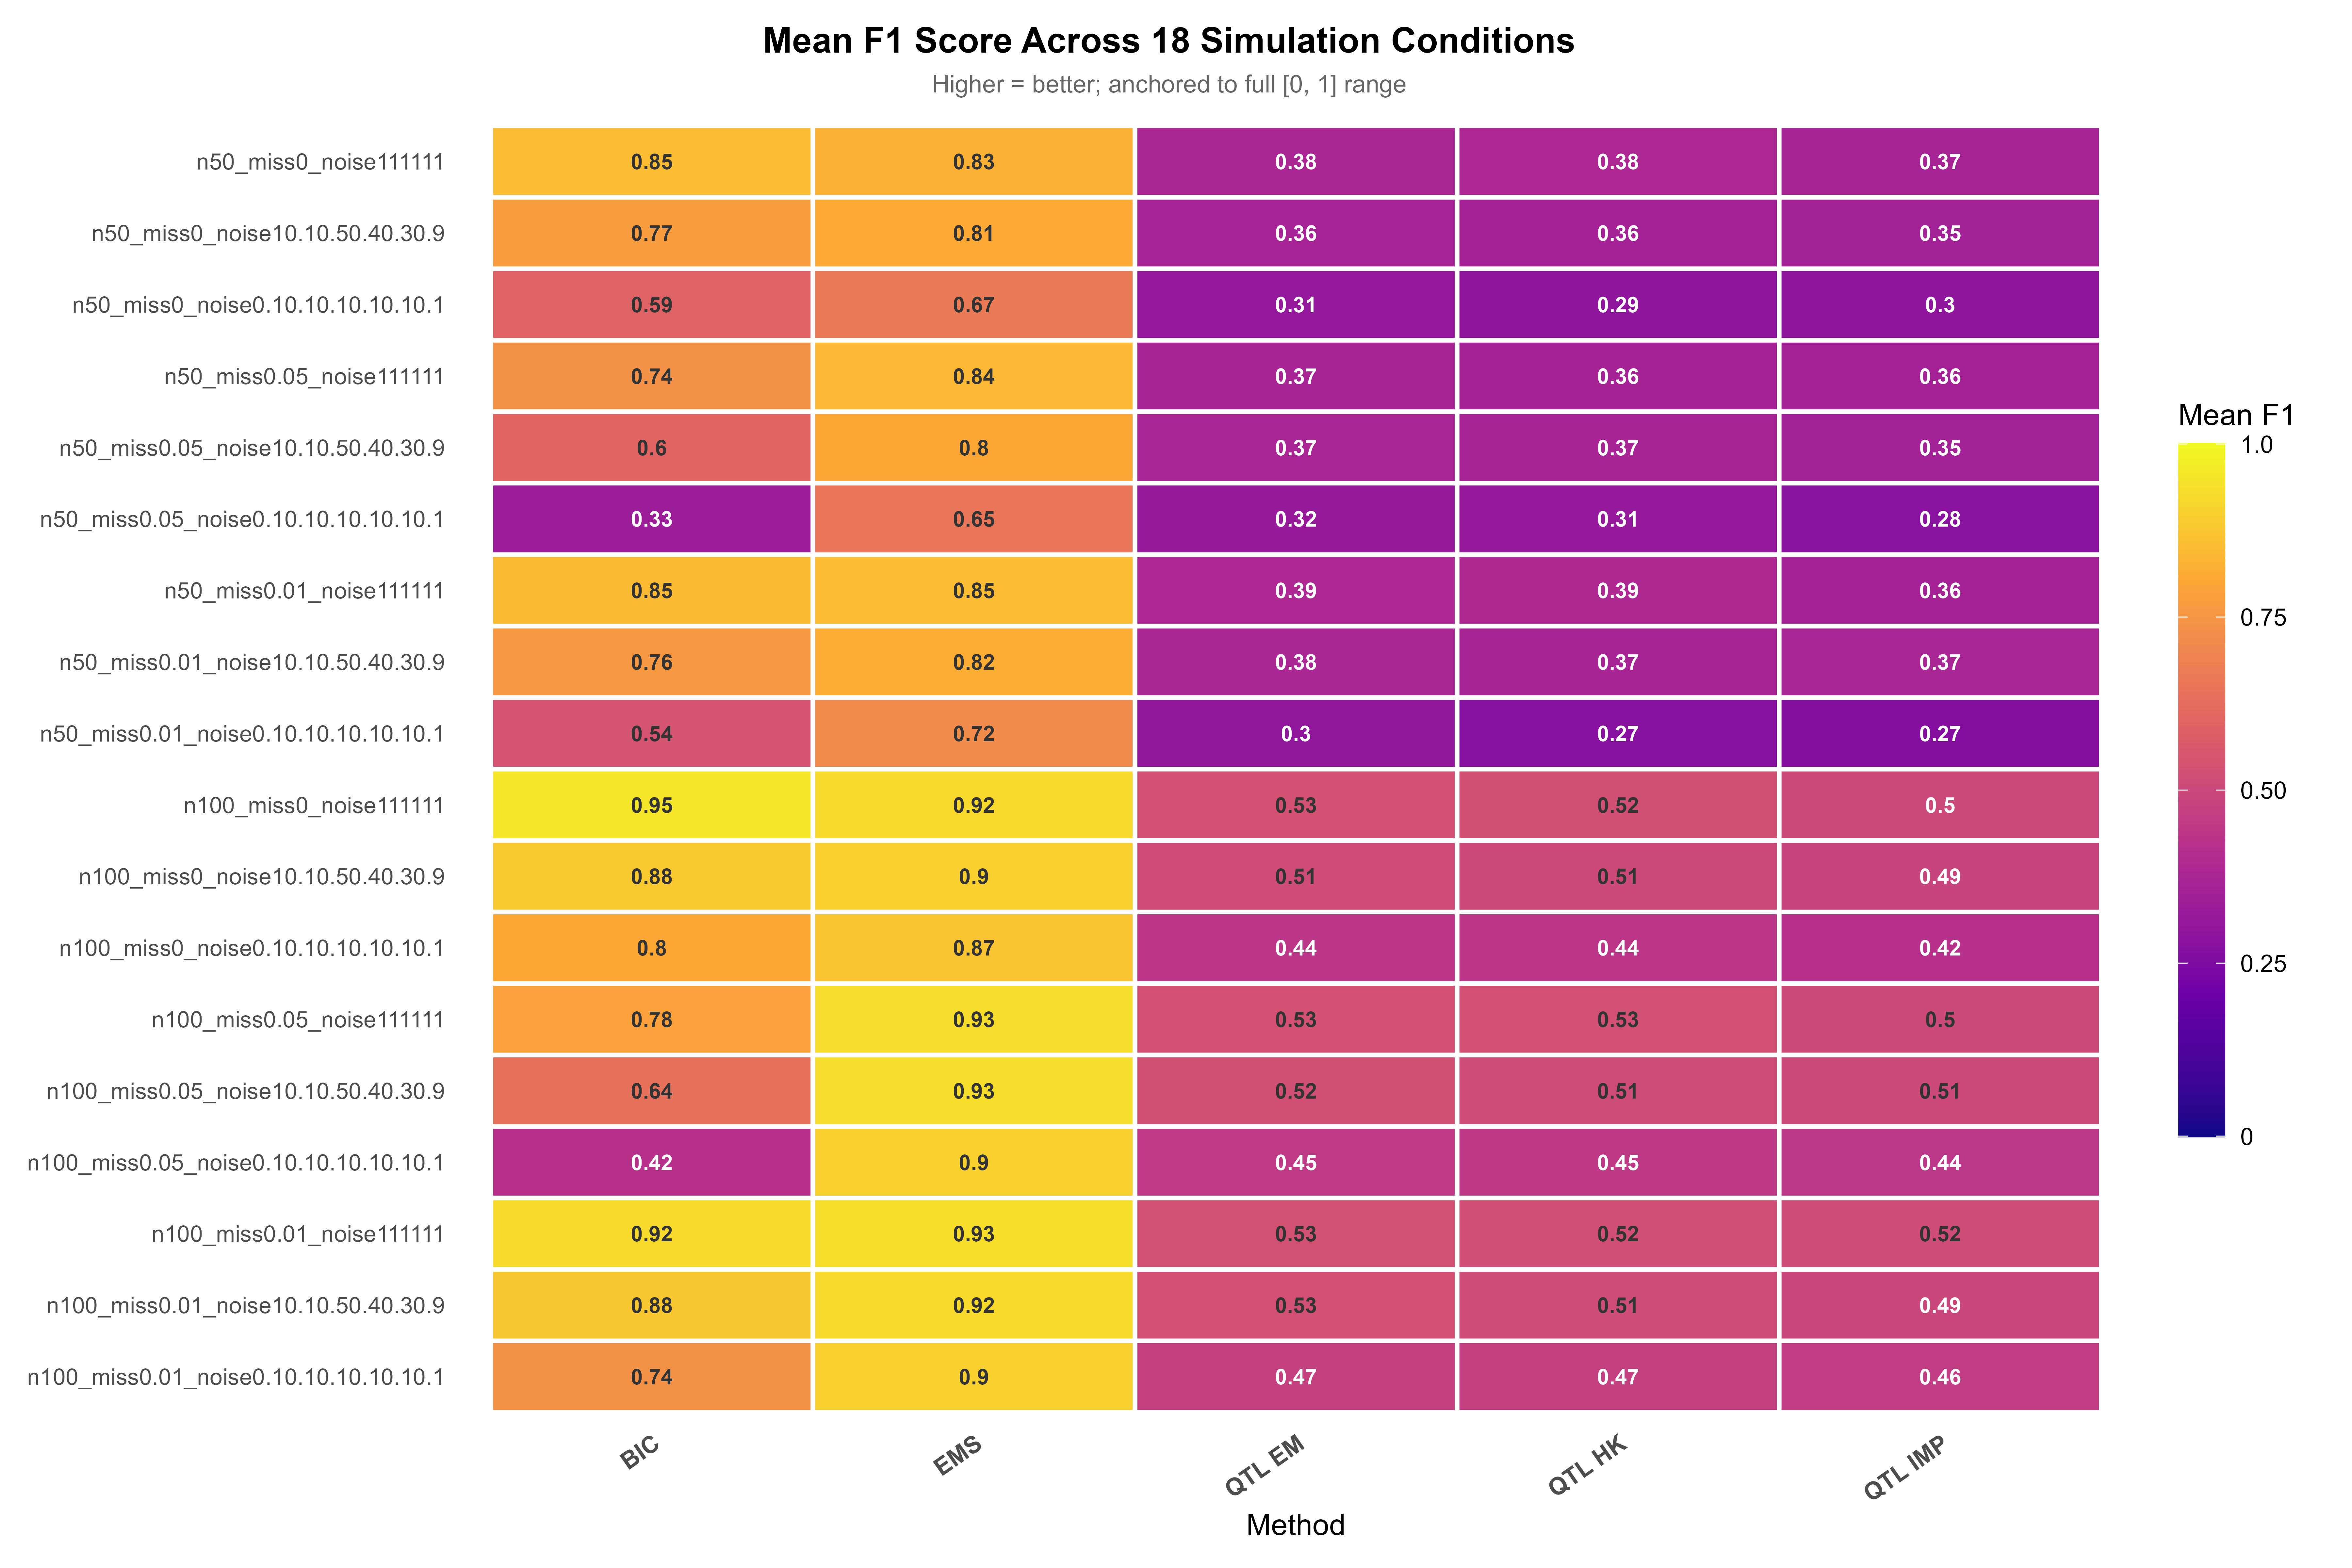
\includegraphics[width=1\linewidth]{./SuppFig_heatmap} \caption{Mean F1 score across 18 simulation conditions. Higher values indicate better performance. Methods include Bayesian Information Criterion (BIC), Expectation-Maximization Selection (E-MS), and three QTL mapping approaches (EM, Haley-Knott, and multiple imputation) evaluated across uniform strong, uniform weak, and random missingness patterns at missingness rates of 0.01, 0.05, and naive 0.10 with sample sizes of n=50 and n=100.}\label{fig:heatmap}
\end{figure}

\begin{figure}[H]
\centering
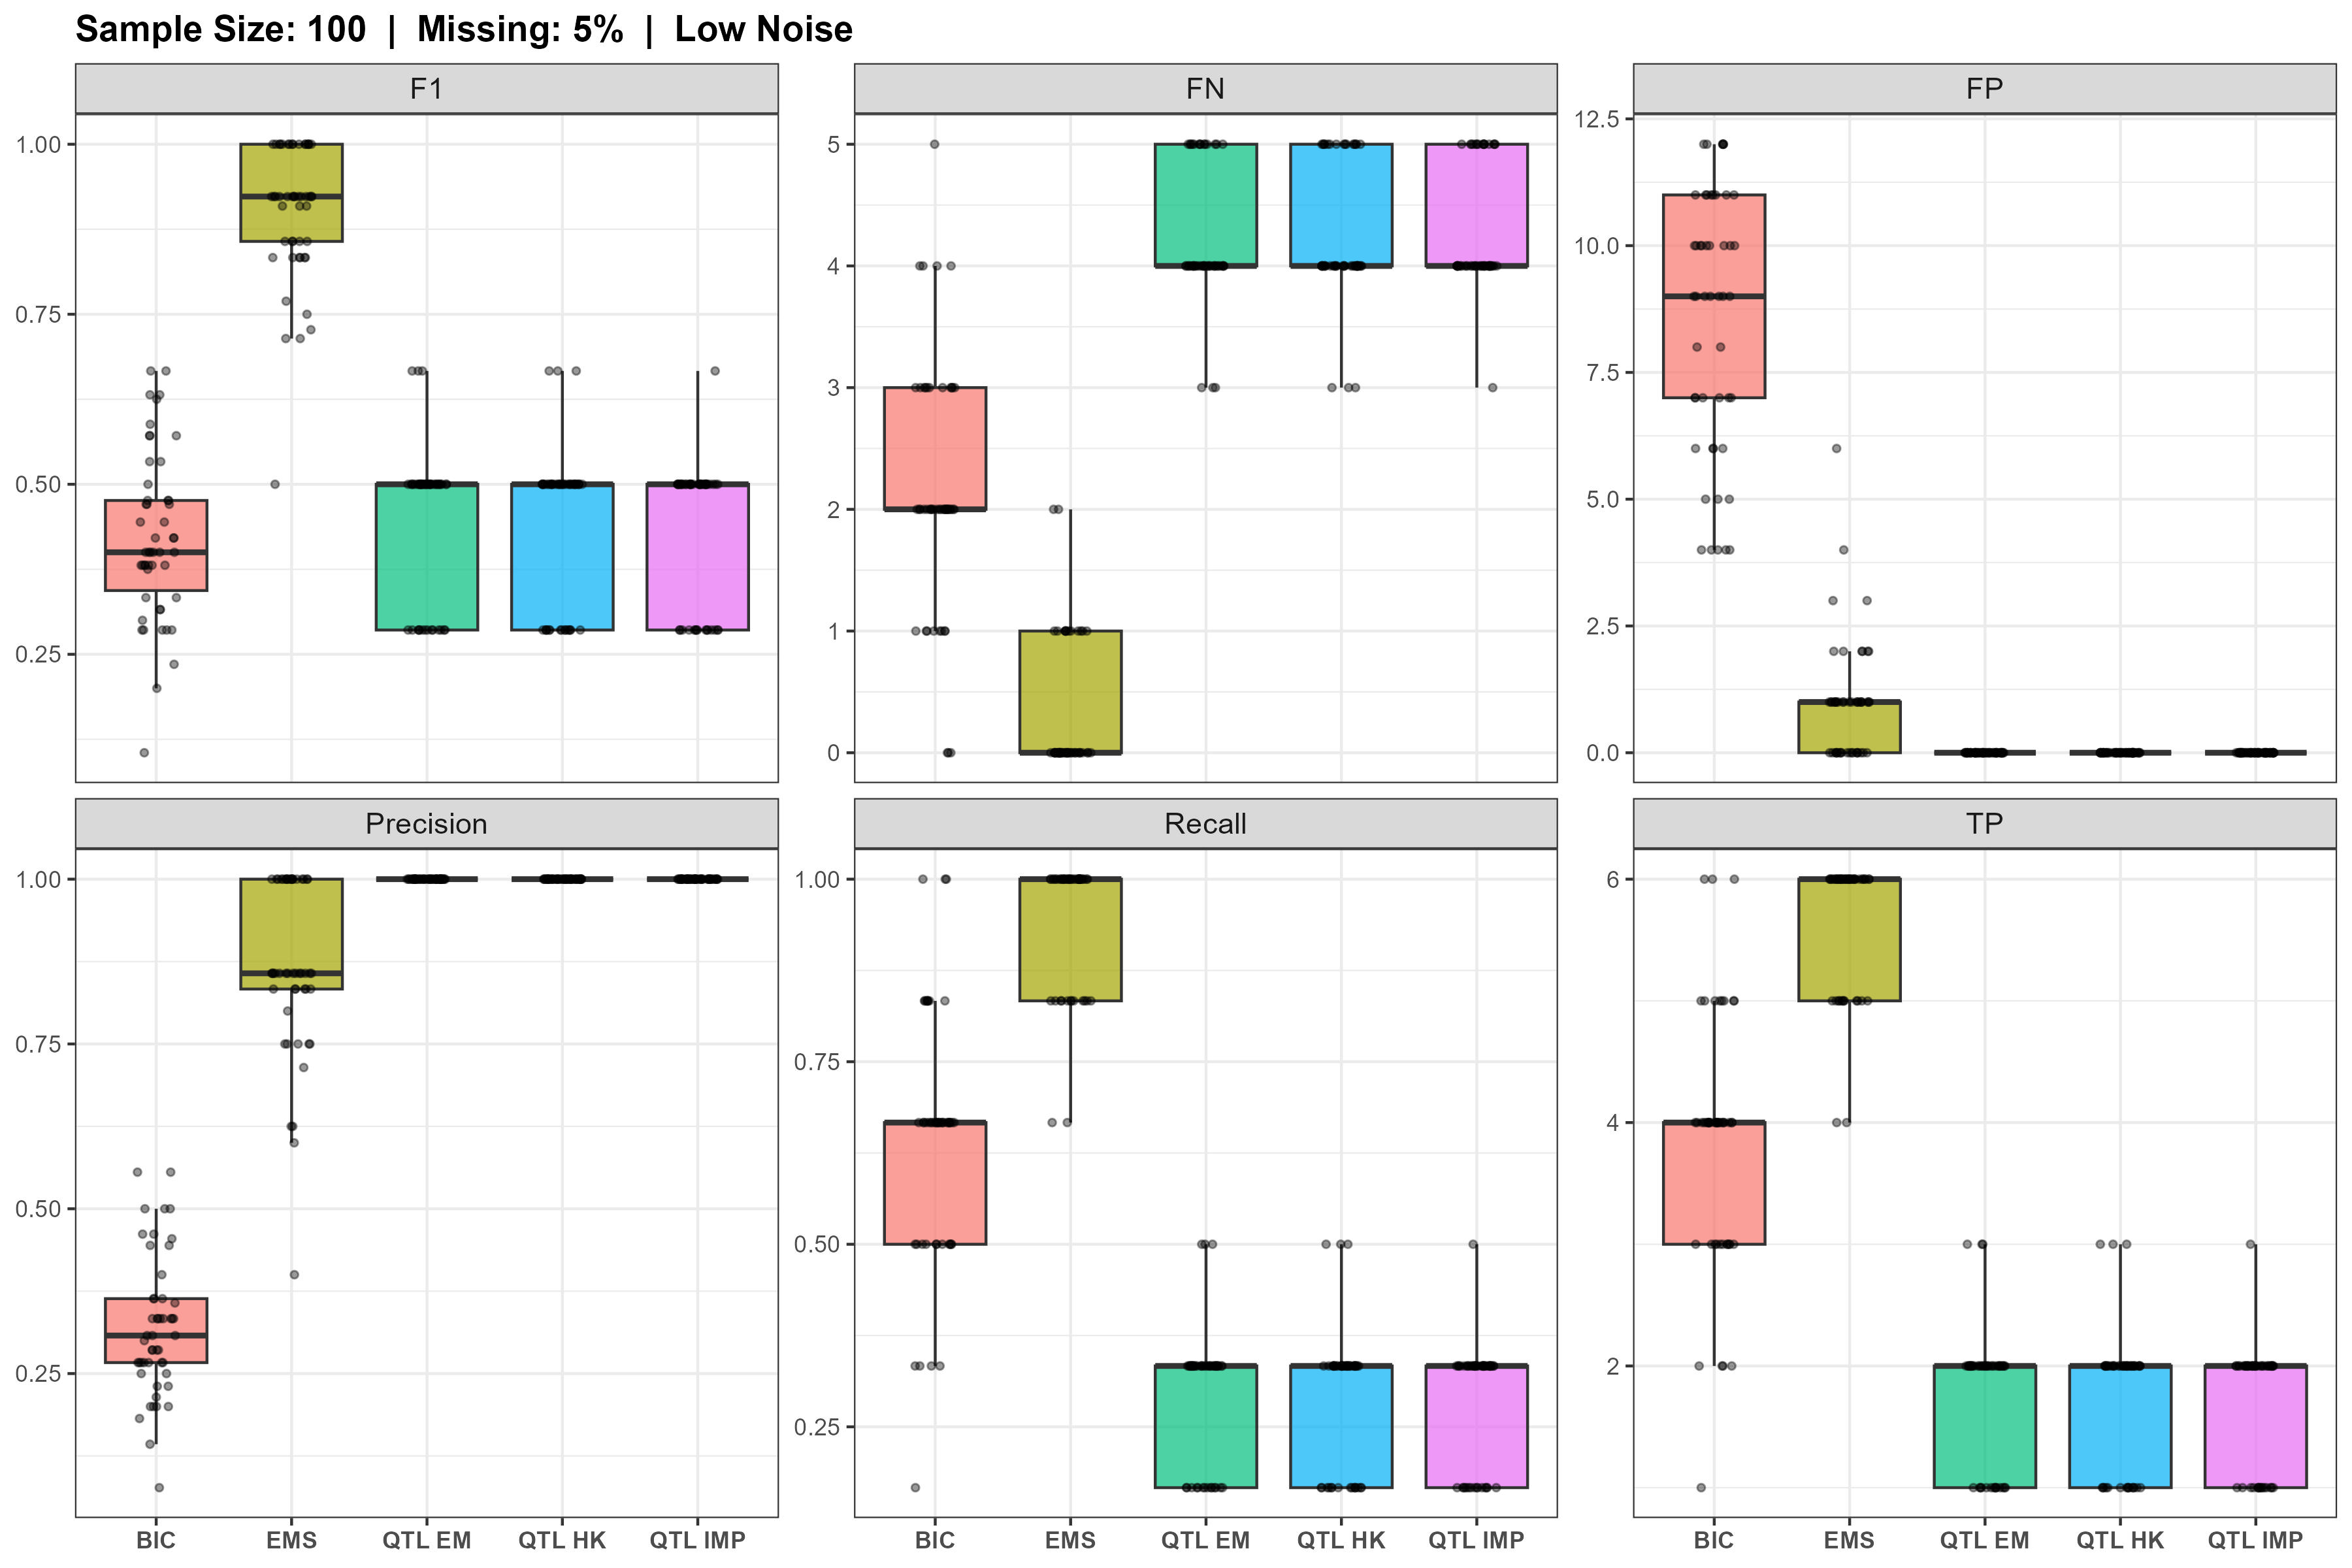
\includegraphics[width=0.95\textwidth,height=0.35\textheight,keepaspectratio]{./SuppFig_sim_n100_miss0.05_noise0.10.10.10.10.10.1.JPG}
\caption{Performance across simulation condition 4. Boxplots comparing F1, FN, FP, Precision, Recall, and TP metrics across baseline (BIC) and four alternative methods (EMS, QTL EM, QTL HK, QTL IMP) under low noise conditions with 5\% missing data (sample size: 100).}
\label{fig:sim4}
\end{figure}


\clearpage


\section{Appendix}

\begin{figure}[H]
\centering
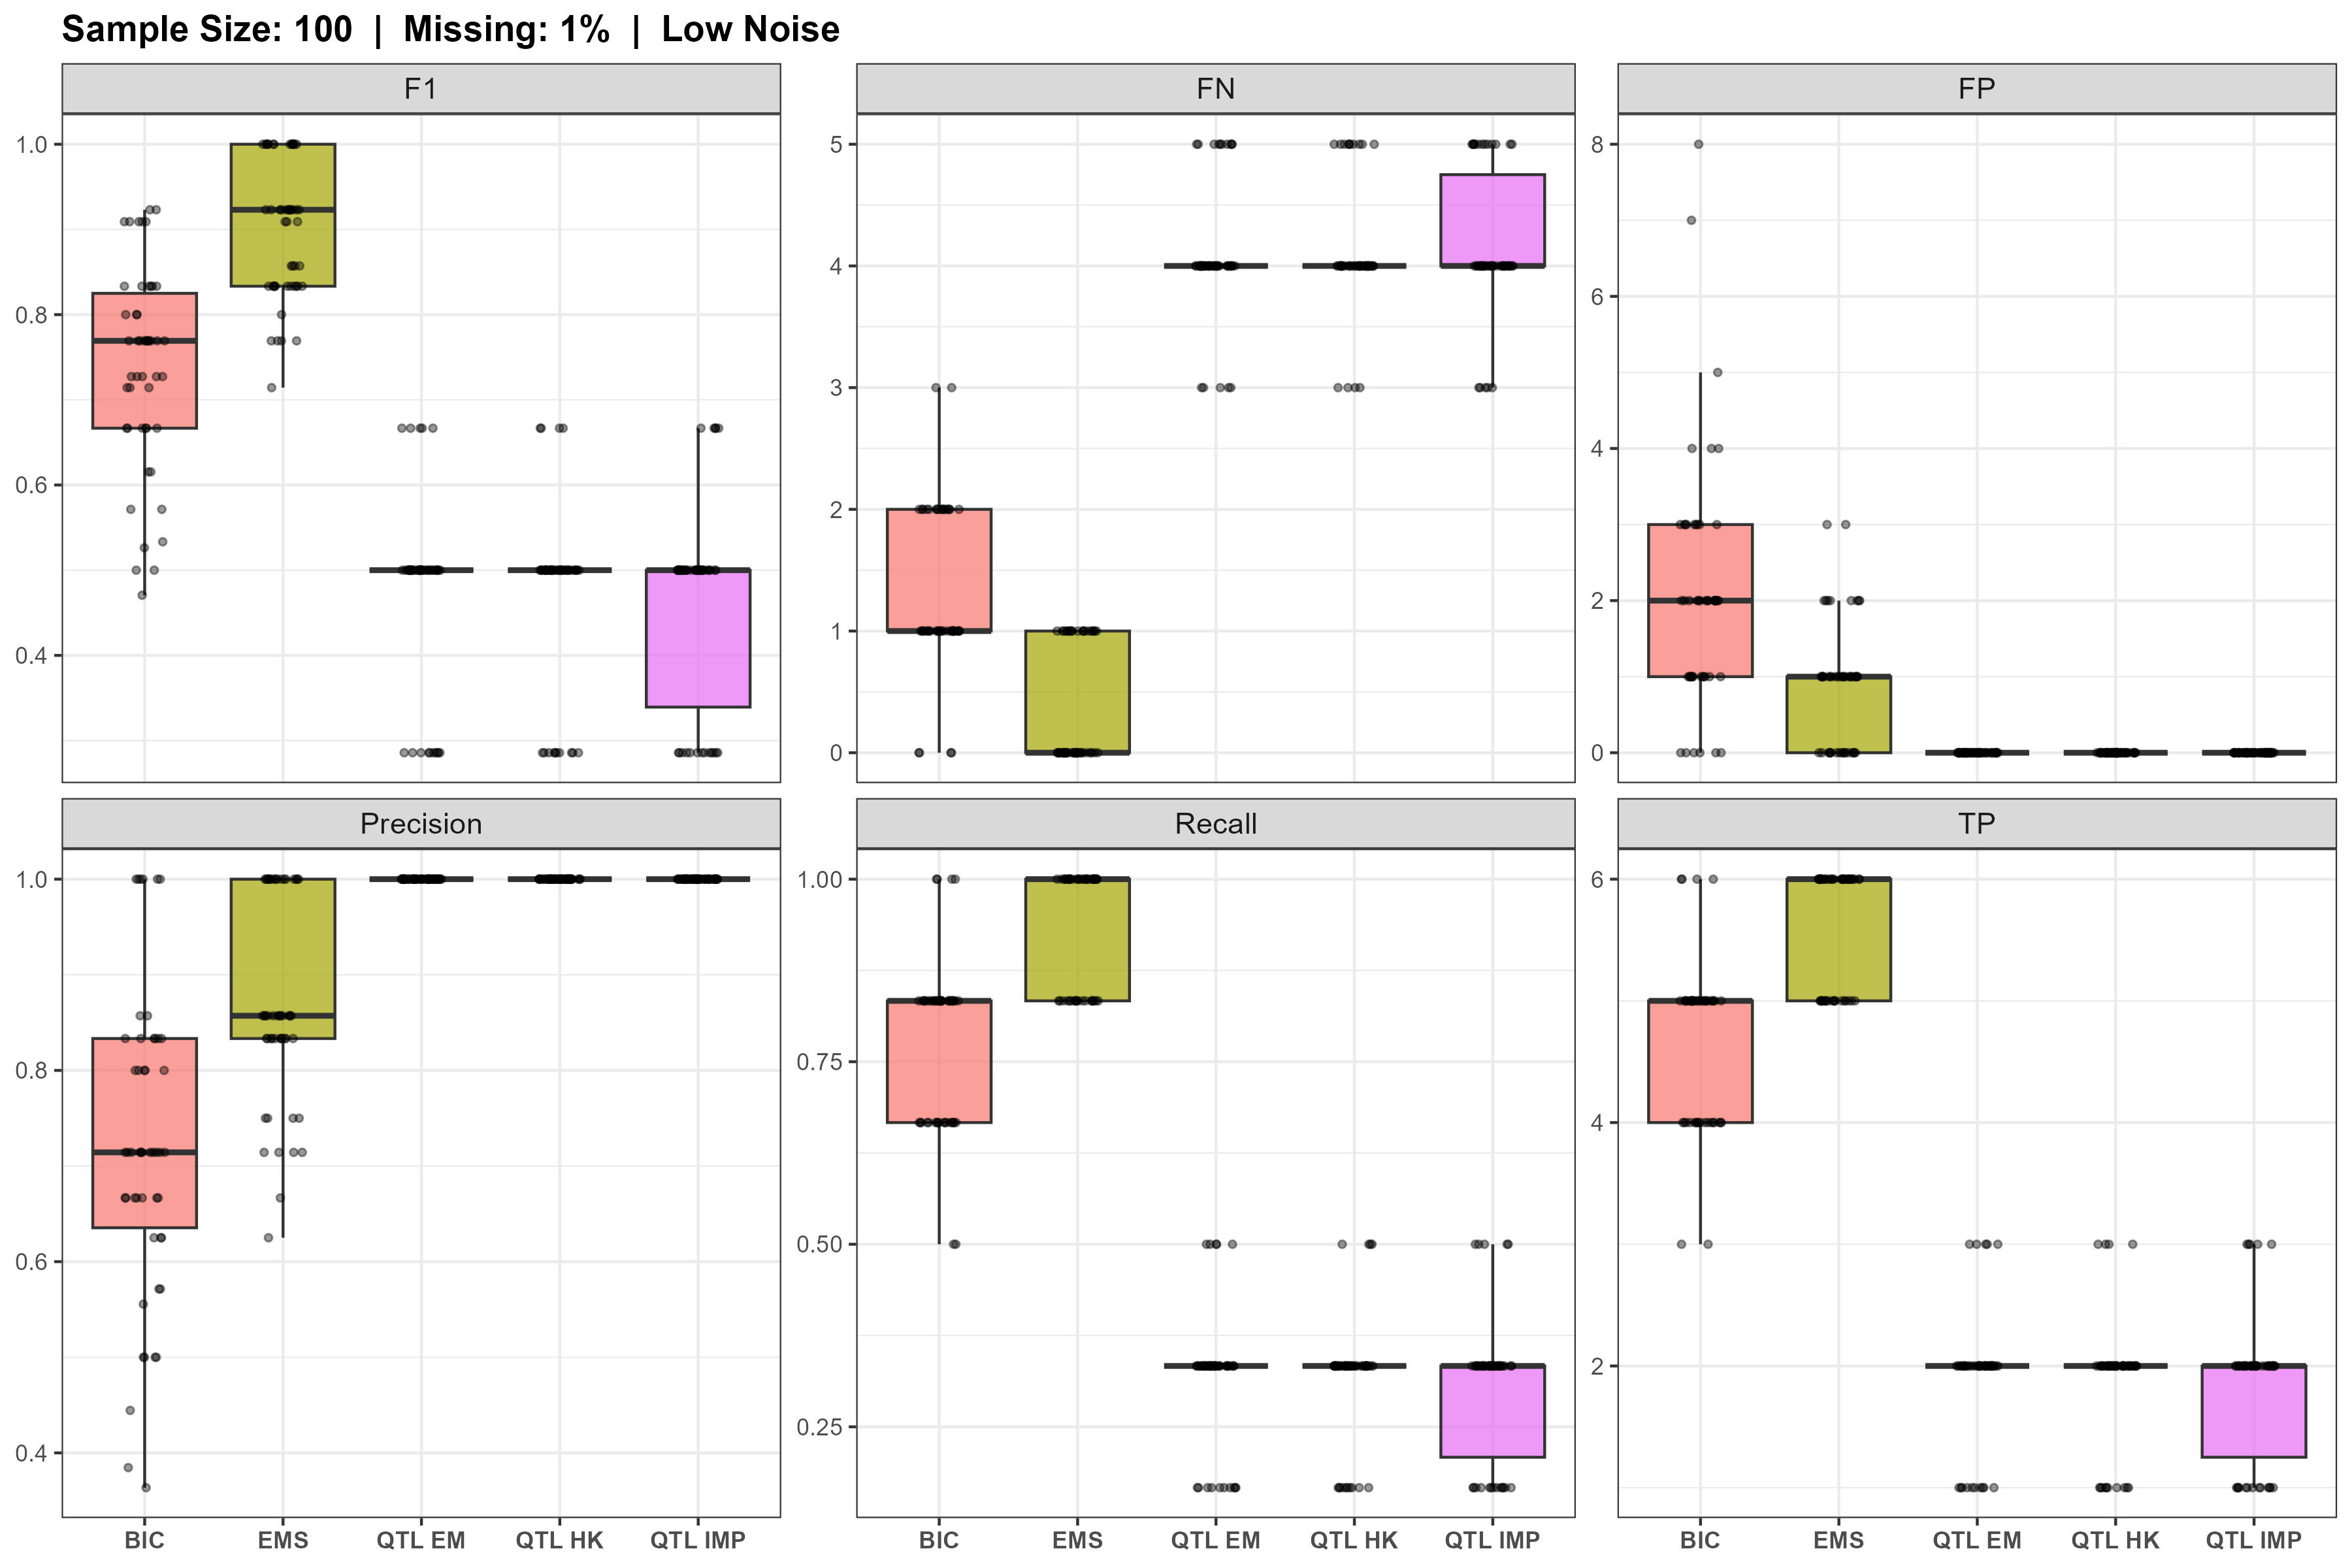
\includegraphics[width=0.95\textwidth,height=0.35\textheight,keepaspectratio]{./SuppFig_sim_n100_miss0.01_noise0.10.10.10.10.10.1.JPG}
\caption{Performance across simulation condition 1. Boxplots comparing F1, FN, FP, Precision, Recall, and TP metrics across baseline (BIC) and four alternative methods (EMS, QTL EM, QTL HK, QTL IMP) under low noise conditions with 1\% missing data (sample size: 100).}
\label{fig:sim1}

\vspace{0.5cm}

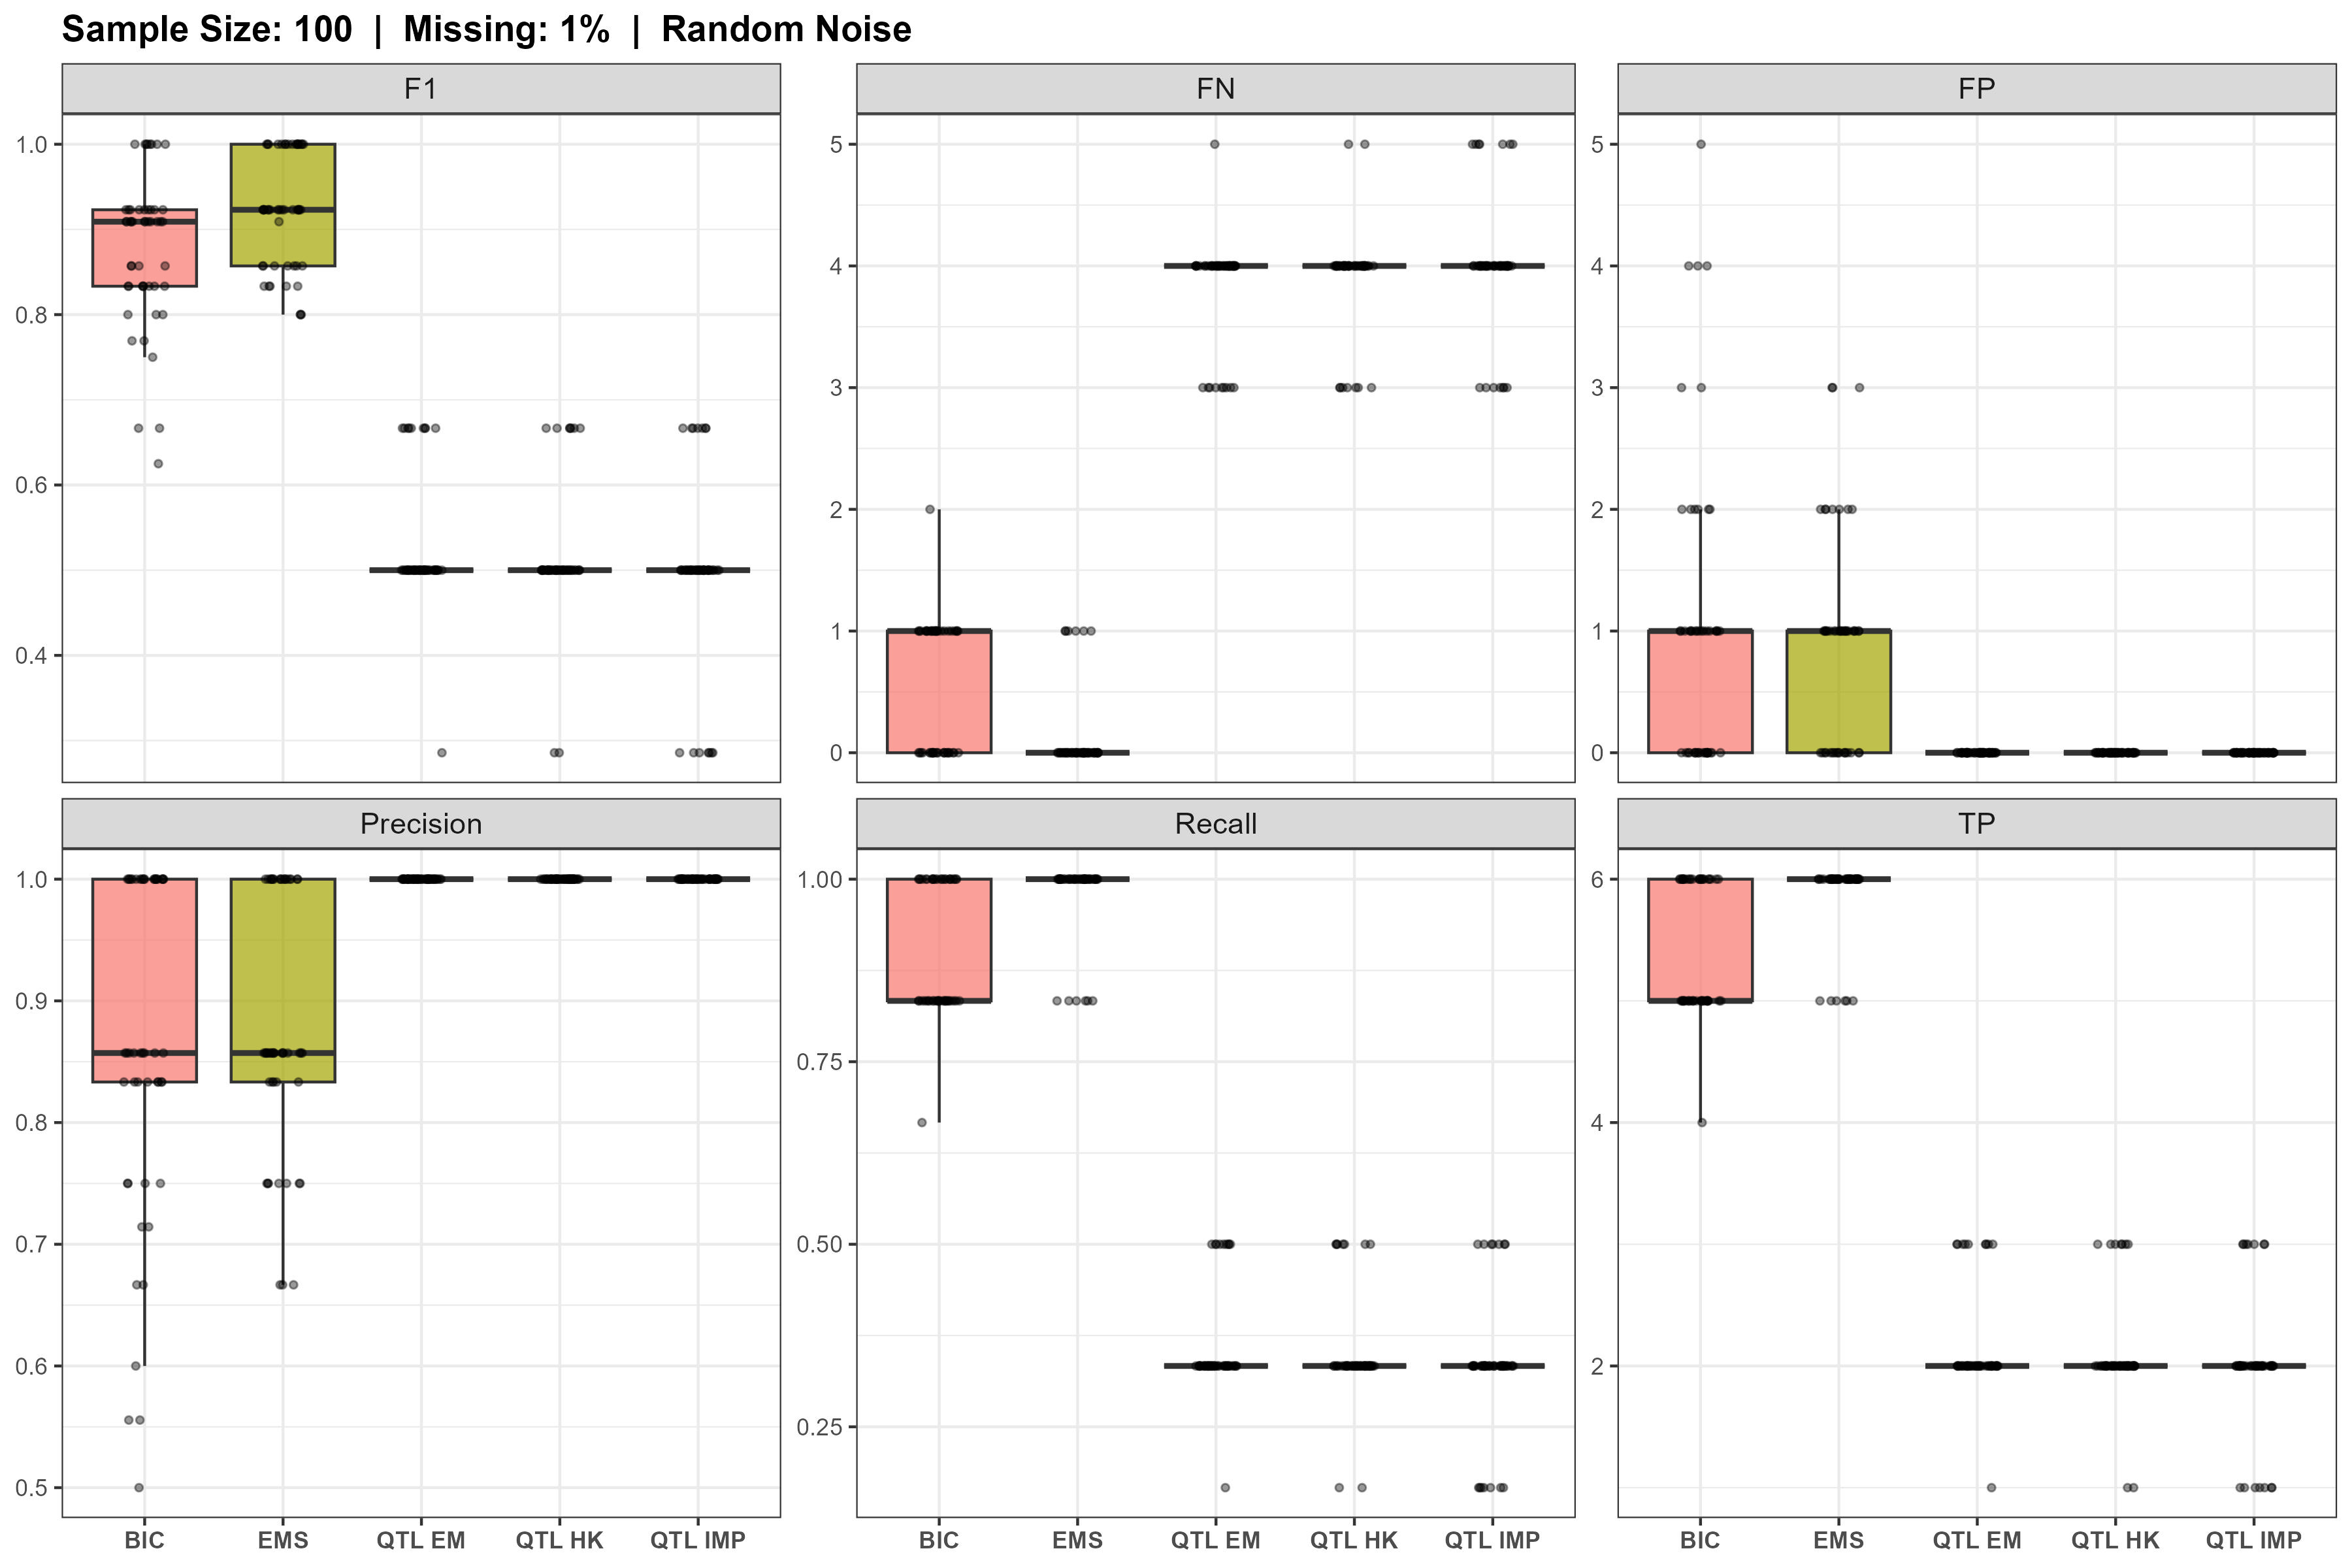
\includegraphics[width=0.95\textwidth,height=0.35\textheight,keepaspectratio]{./SuppFig_sim_n100_miss0.01_noise10.10.50.40.30.9.JPG}
\caption{Performance across simulation condition 2. Boxplots comparing F1, FN, FP, Precision, Recall, and TP metrics across baseline (BIC) and four alternative methods (EMS, QTL EM, QTL HK, QTL IMP) under random noise conditions with 1\% missing data (sample size: 100). QTL variants show more variable performance compared to EMS.}
\label{fig:sim2}
\end{figure}

\begin{figure}[H]
\centering
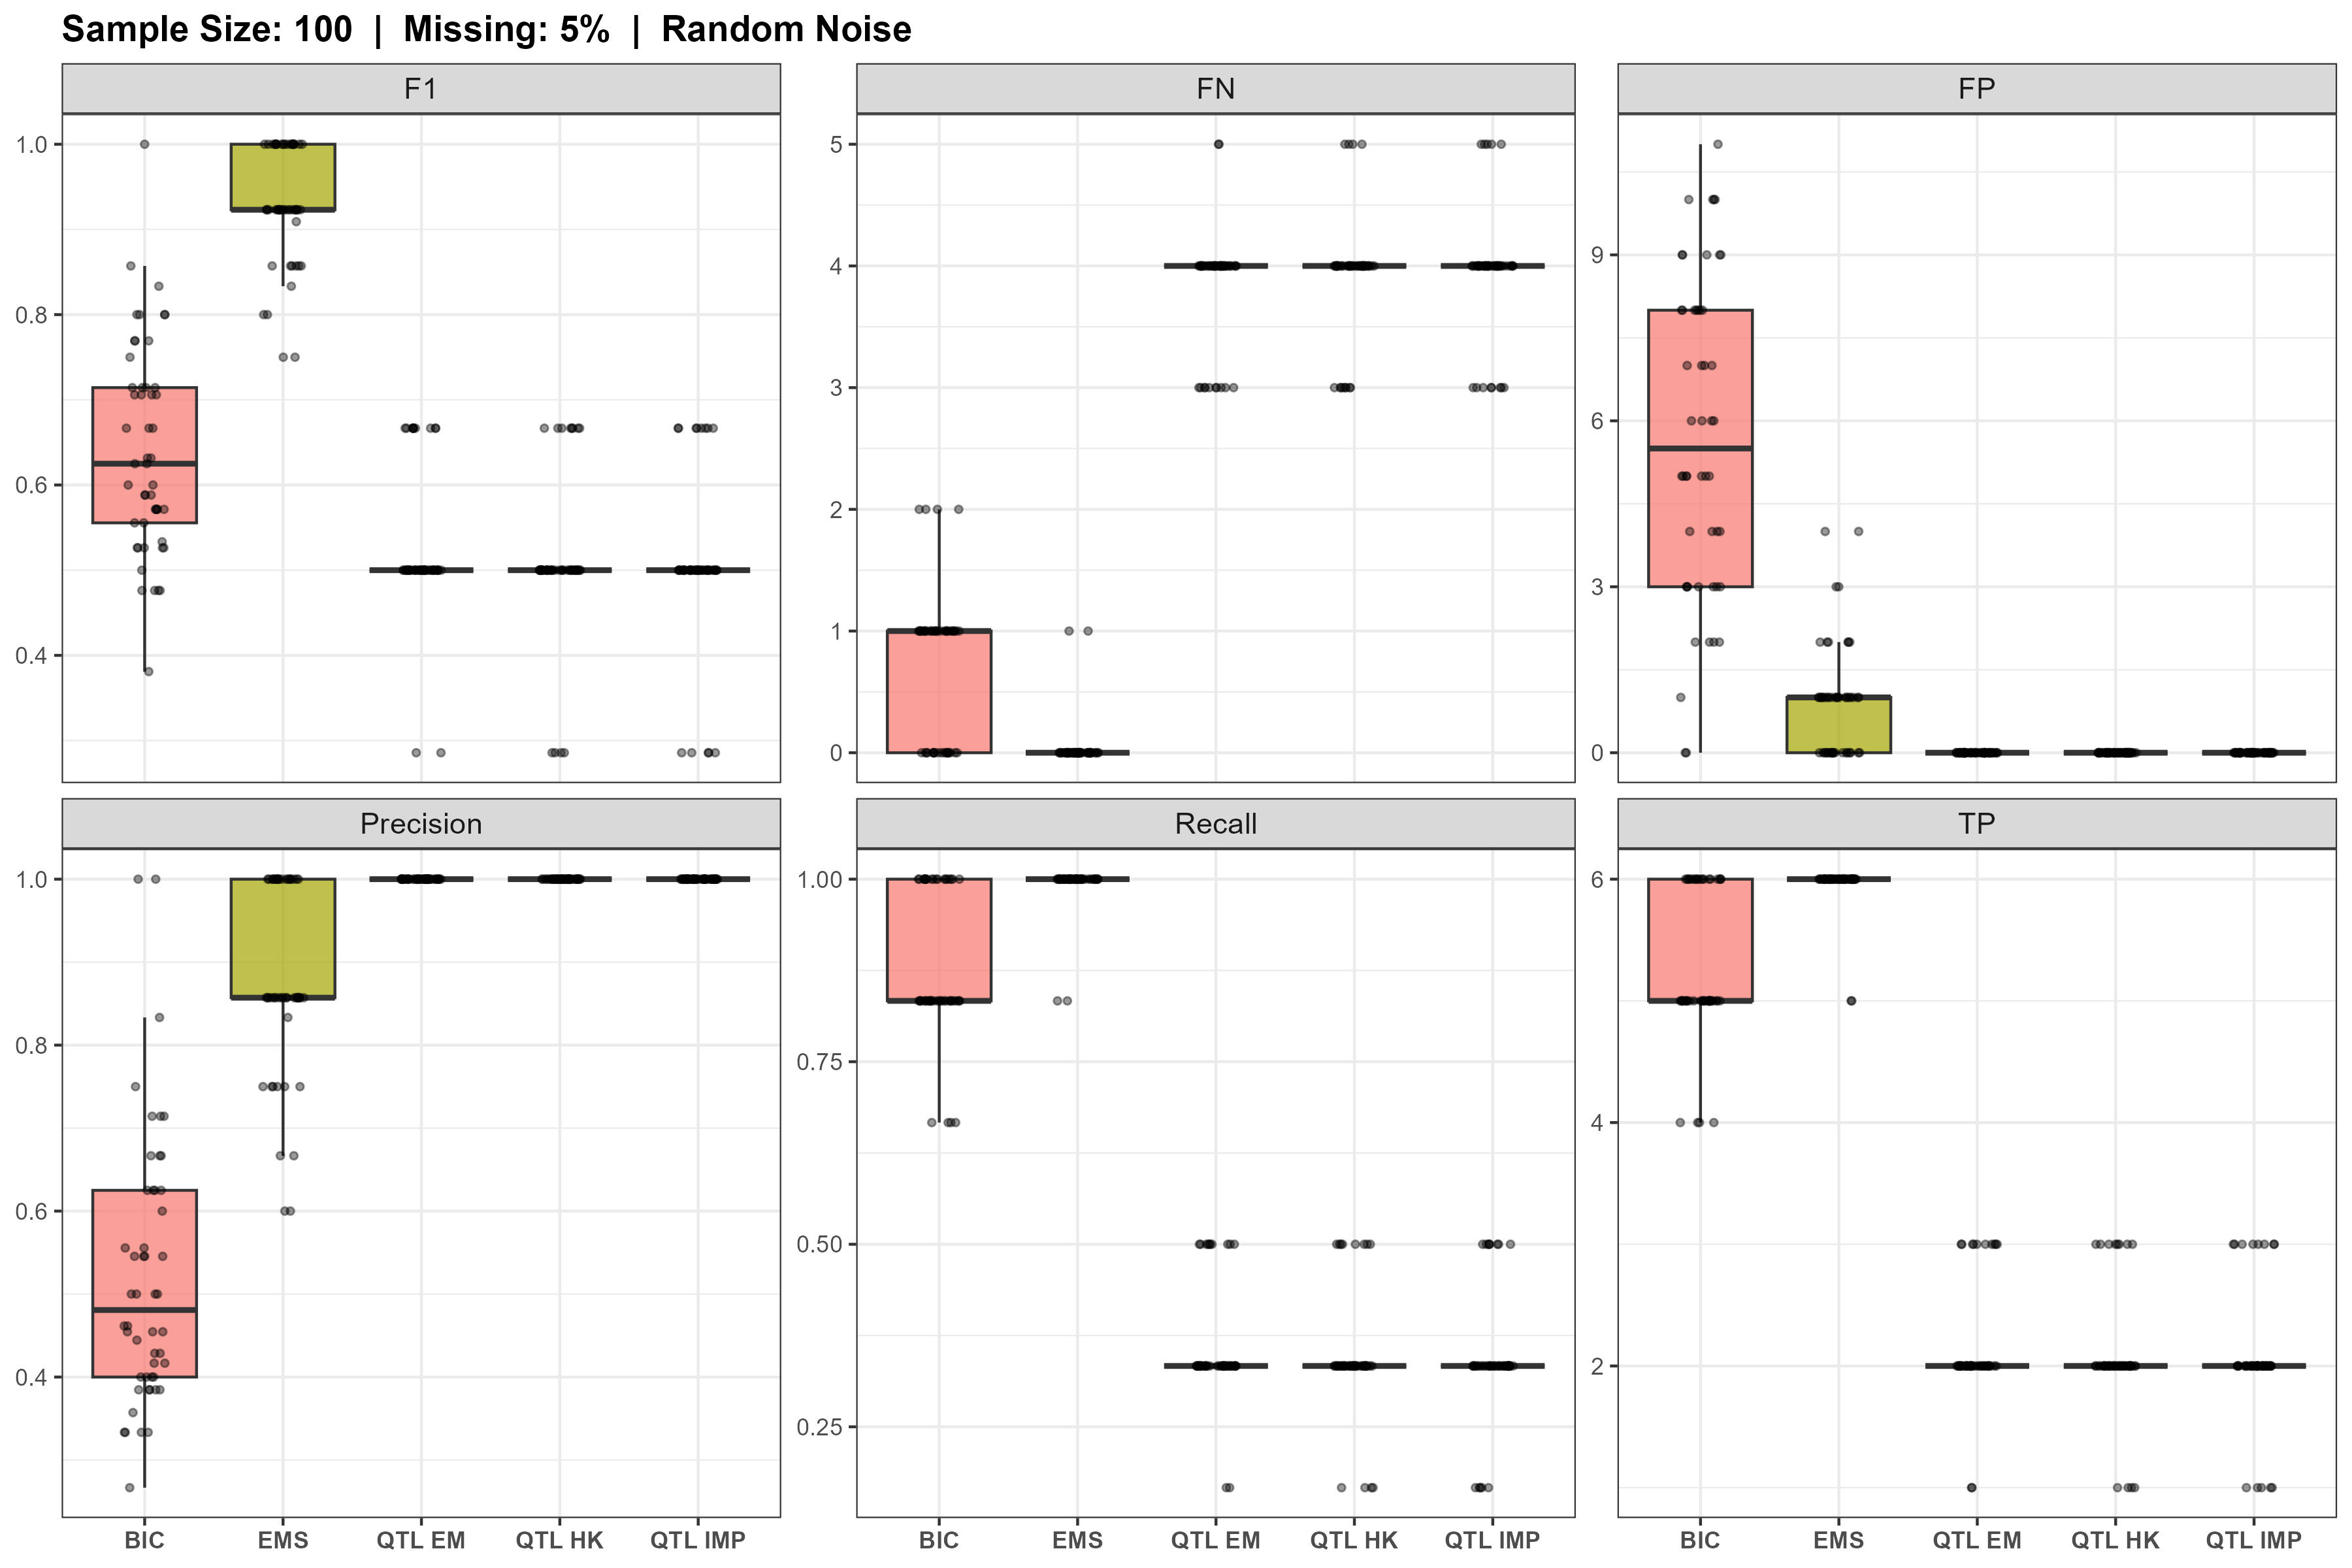
\includegraphics[width=0.95\textwidth,height=0.35\textheight,keepaspectratio]{./SuppFig_sim_n100_miss0.05_noise10.10.50.40.30.9.JPG}
\caption{Performance across simulation condition 5. Boxplots comparing F1, FN, FP, Precision, Recall, and TP metrics across baseline (BIC) and four alternative methods (EMS, QTL EM, QTL HK, QTL IMP) under random noise conditions with 5\% missing data (sample size: 100). EMS shows more consistent performance, while QTL EM exhibits greater variability.}
\label{fig:sim5}

\vspace{0.5cm}

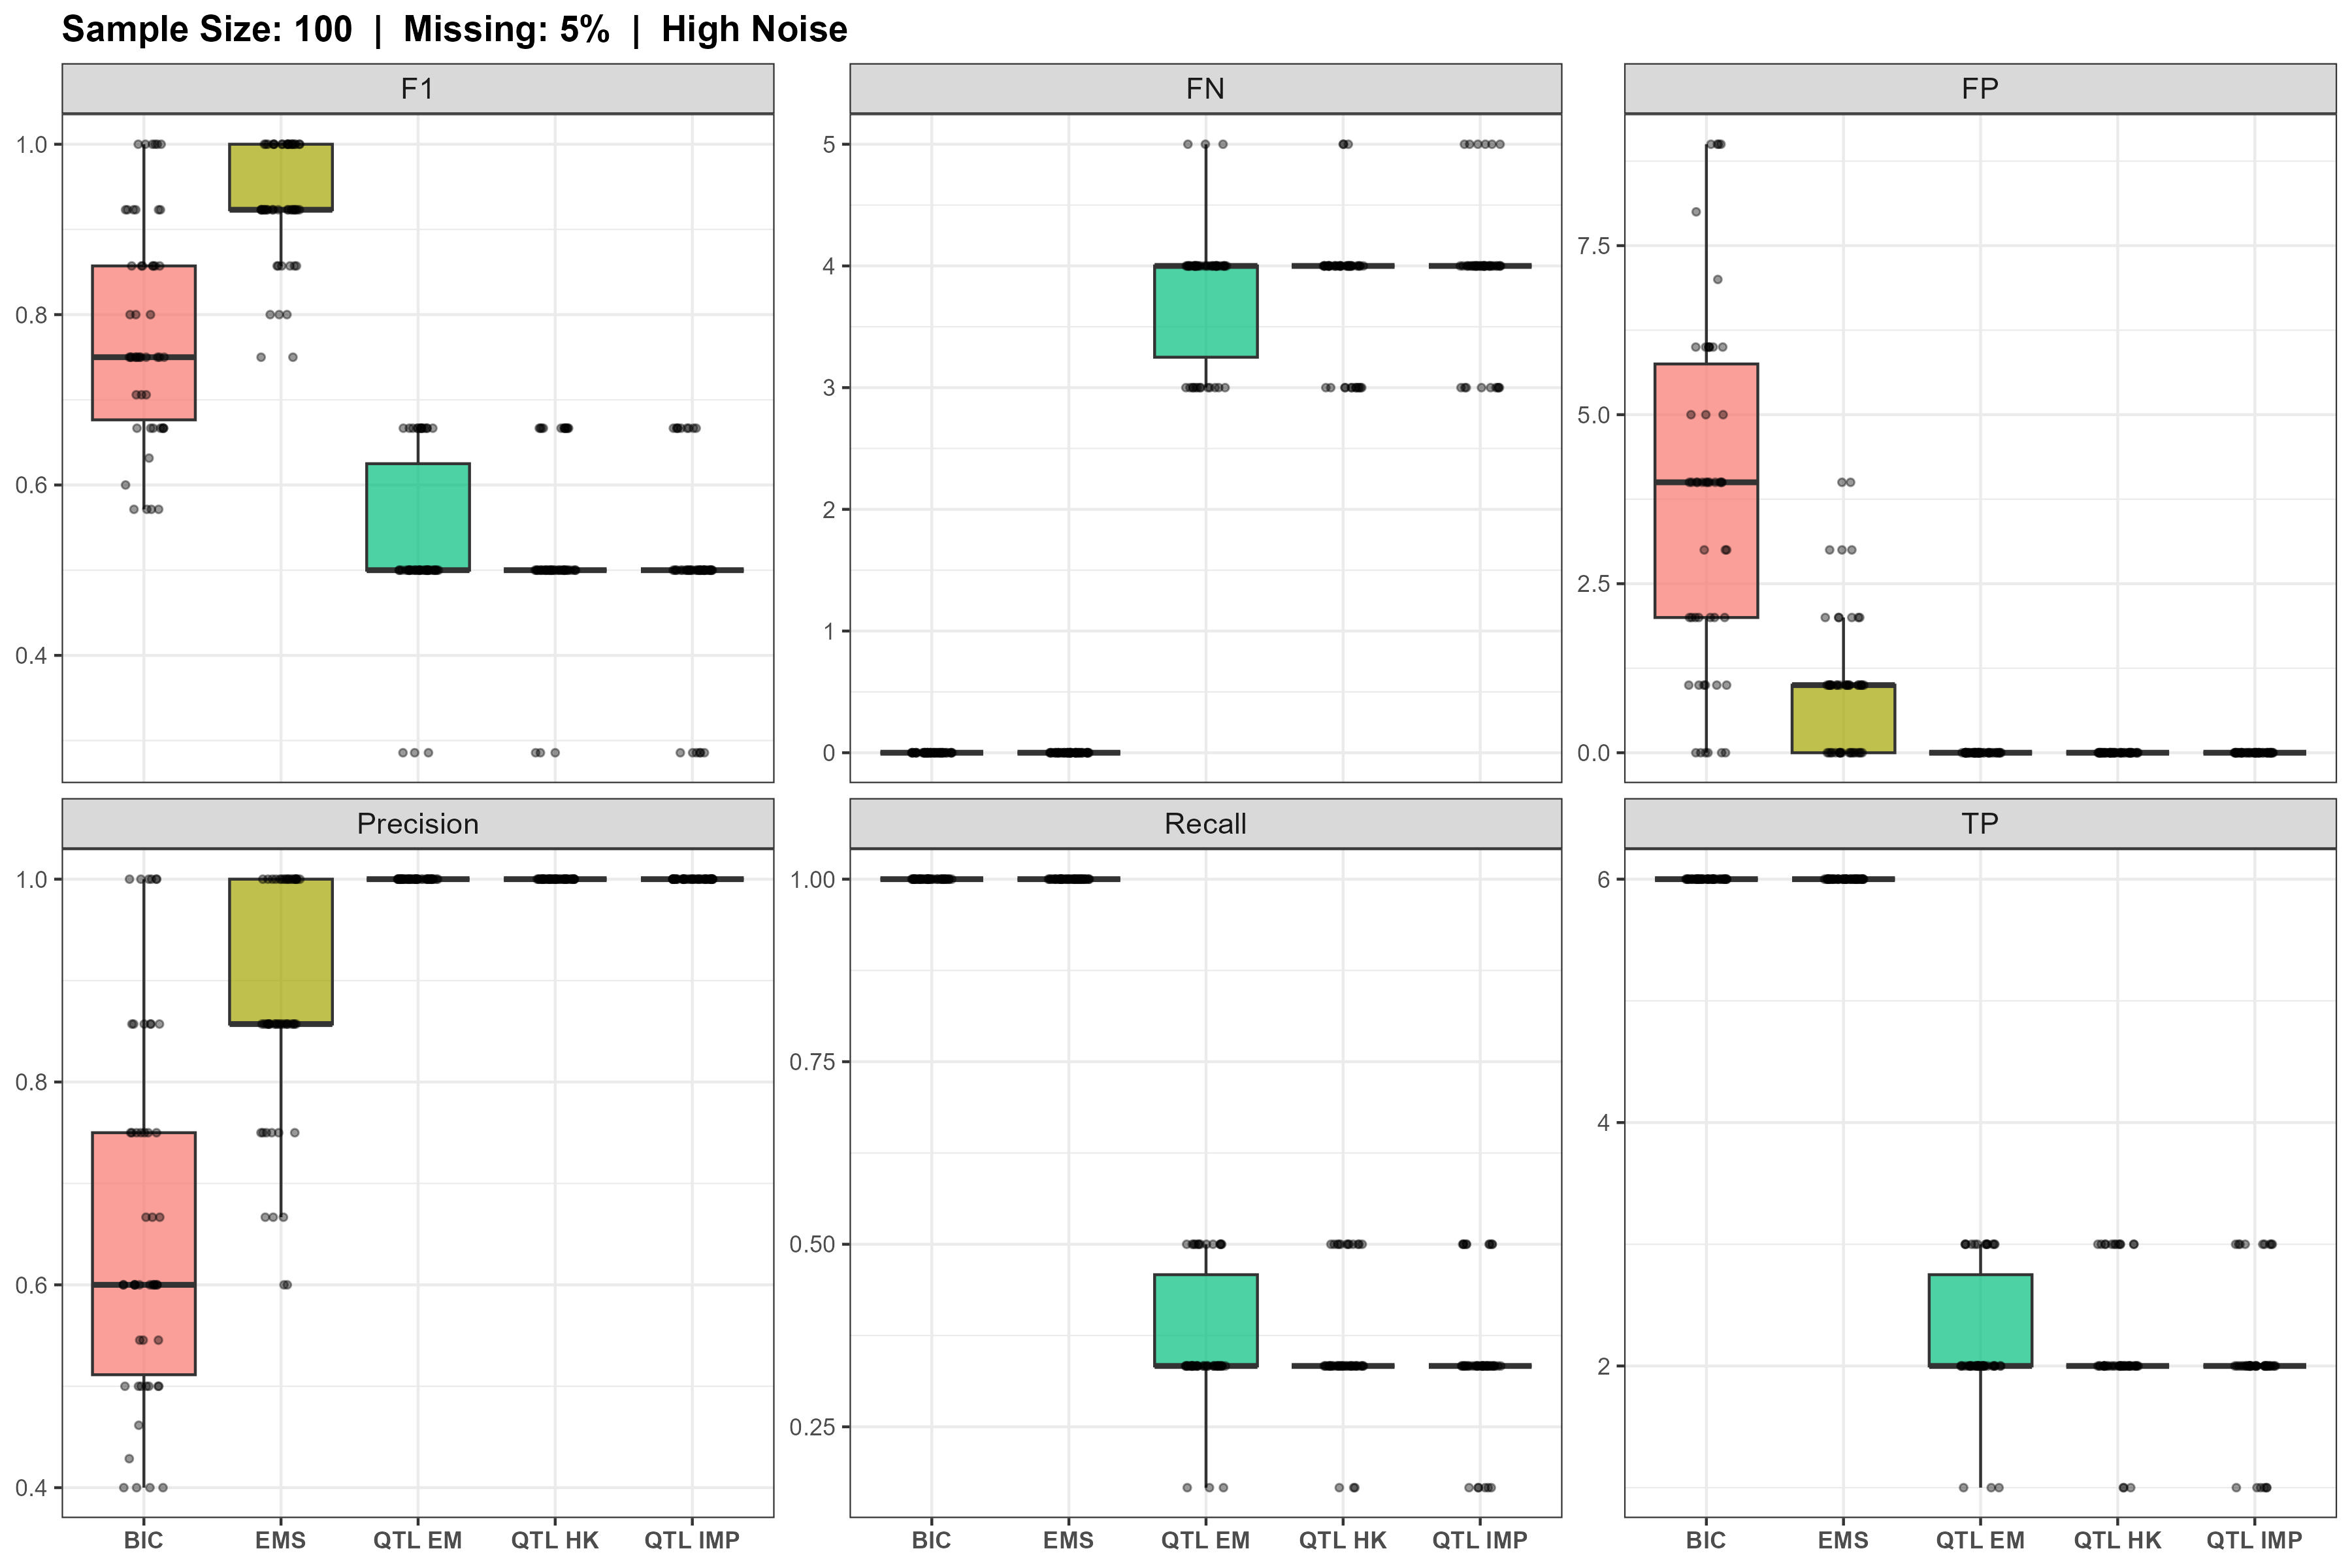
\includegraphics[width=0.95\textwidth,height=0.35\textheight,keepaspectratio]{./SuppFig_sim_n100_miss0.05_noise111111.JPG}
\caption{Performance across simulation condition 6. Boxplots comparing F1, FN, FP, Precision, Recall, and TP metrics across baseline (BIC) and four alternative methods (EMS, QTL EM, QTL HK, QTL IMP) under high noise conditions with 5\% missing data (sample size: 100). QTL HK and QTL IMP maintain superior performance despite increased data missingness.}
\label{fig:sim6}
\end{figure}

\begin{figure}[H]
\centering
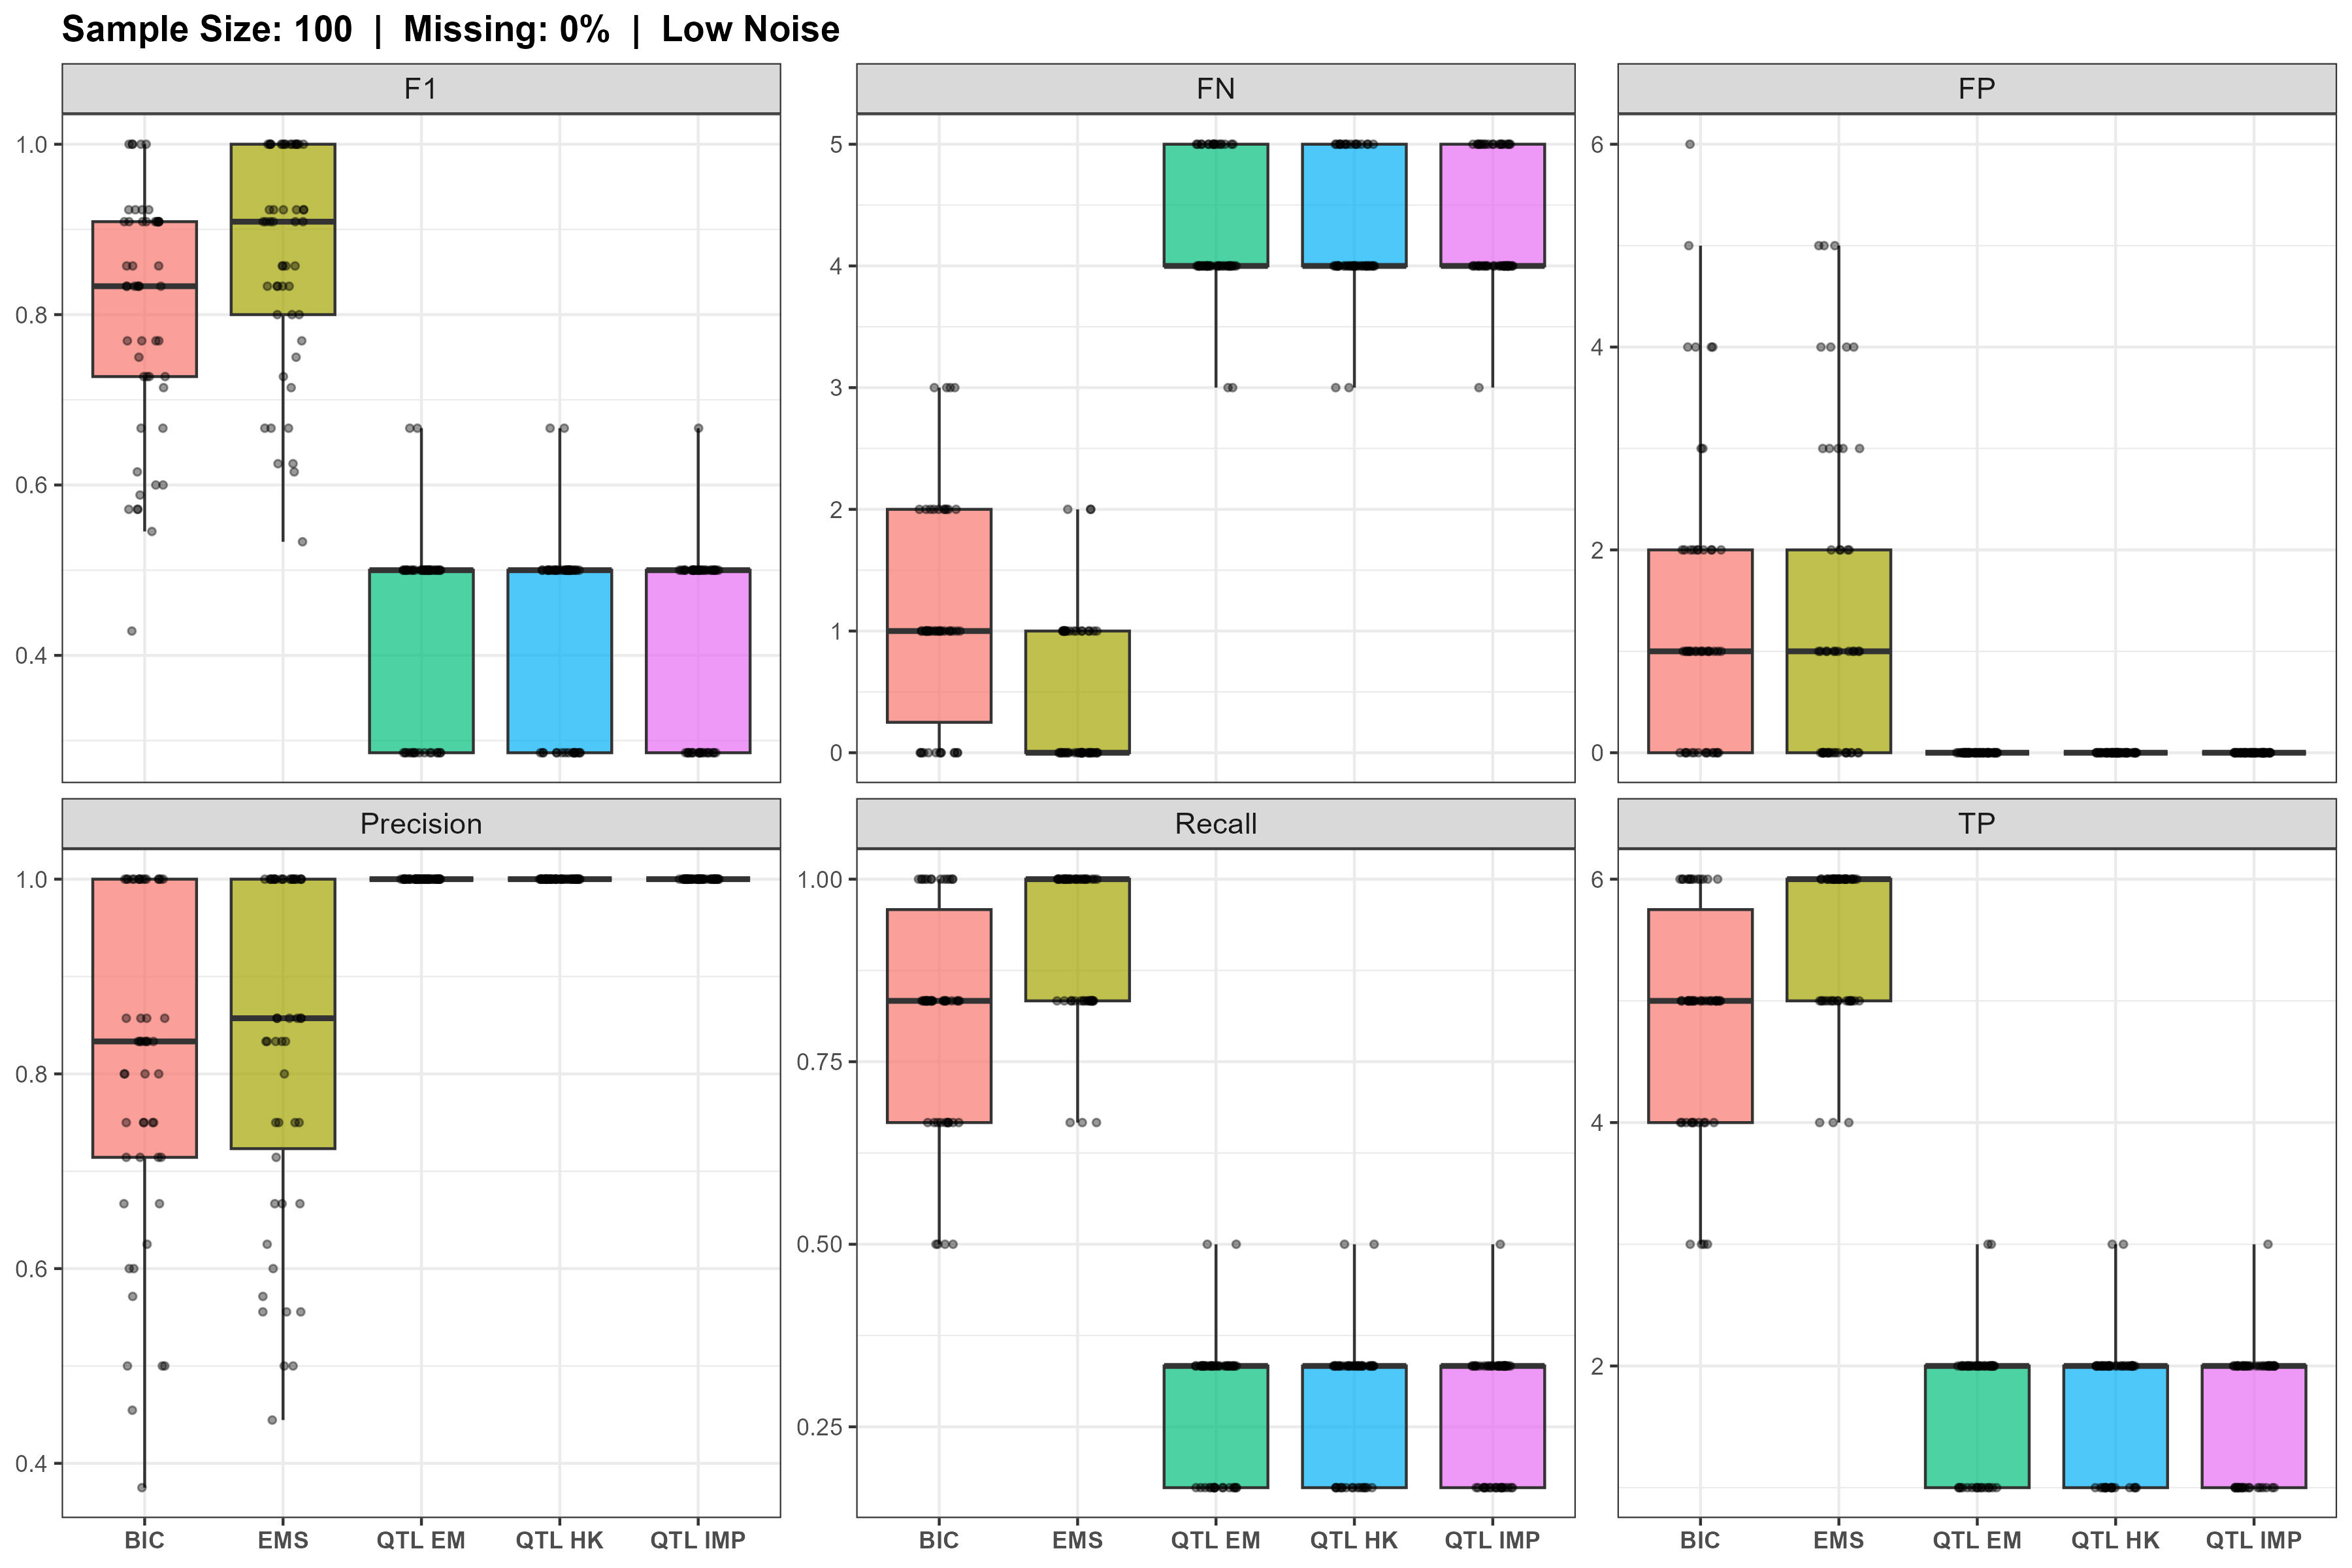
\includegraphics[width=0.95\textwidth,height=0.35\textheight,keepaspectratio]{./SuppFig_sim_n100_miss0_noise0.10.10.10.10.10.1.JPG}
\caption{Performance across simulation condition 7. Boxplots comparing F1, FN, FP, Precision, Recall, and TP metrics across baseline (BIC) and four alternative methods (EMS, QTL EM, QTL HK, QTL IMP) under low noise conditions with 0\% missing data (sample size: 100).}
\label{fig:sim7}

\vspace{0.5cm}

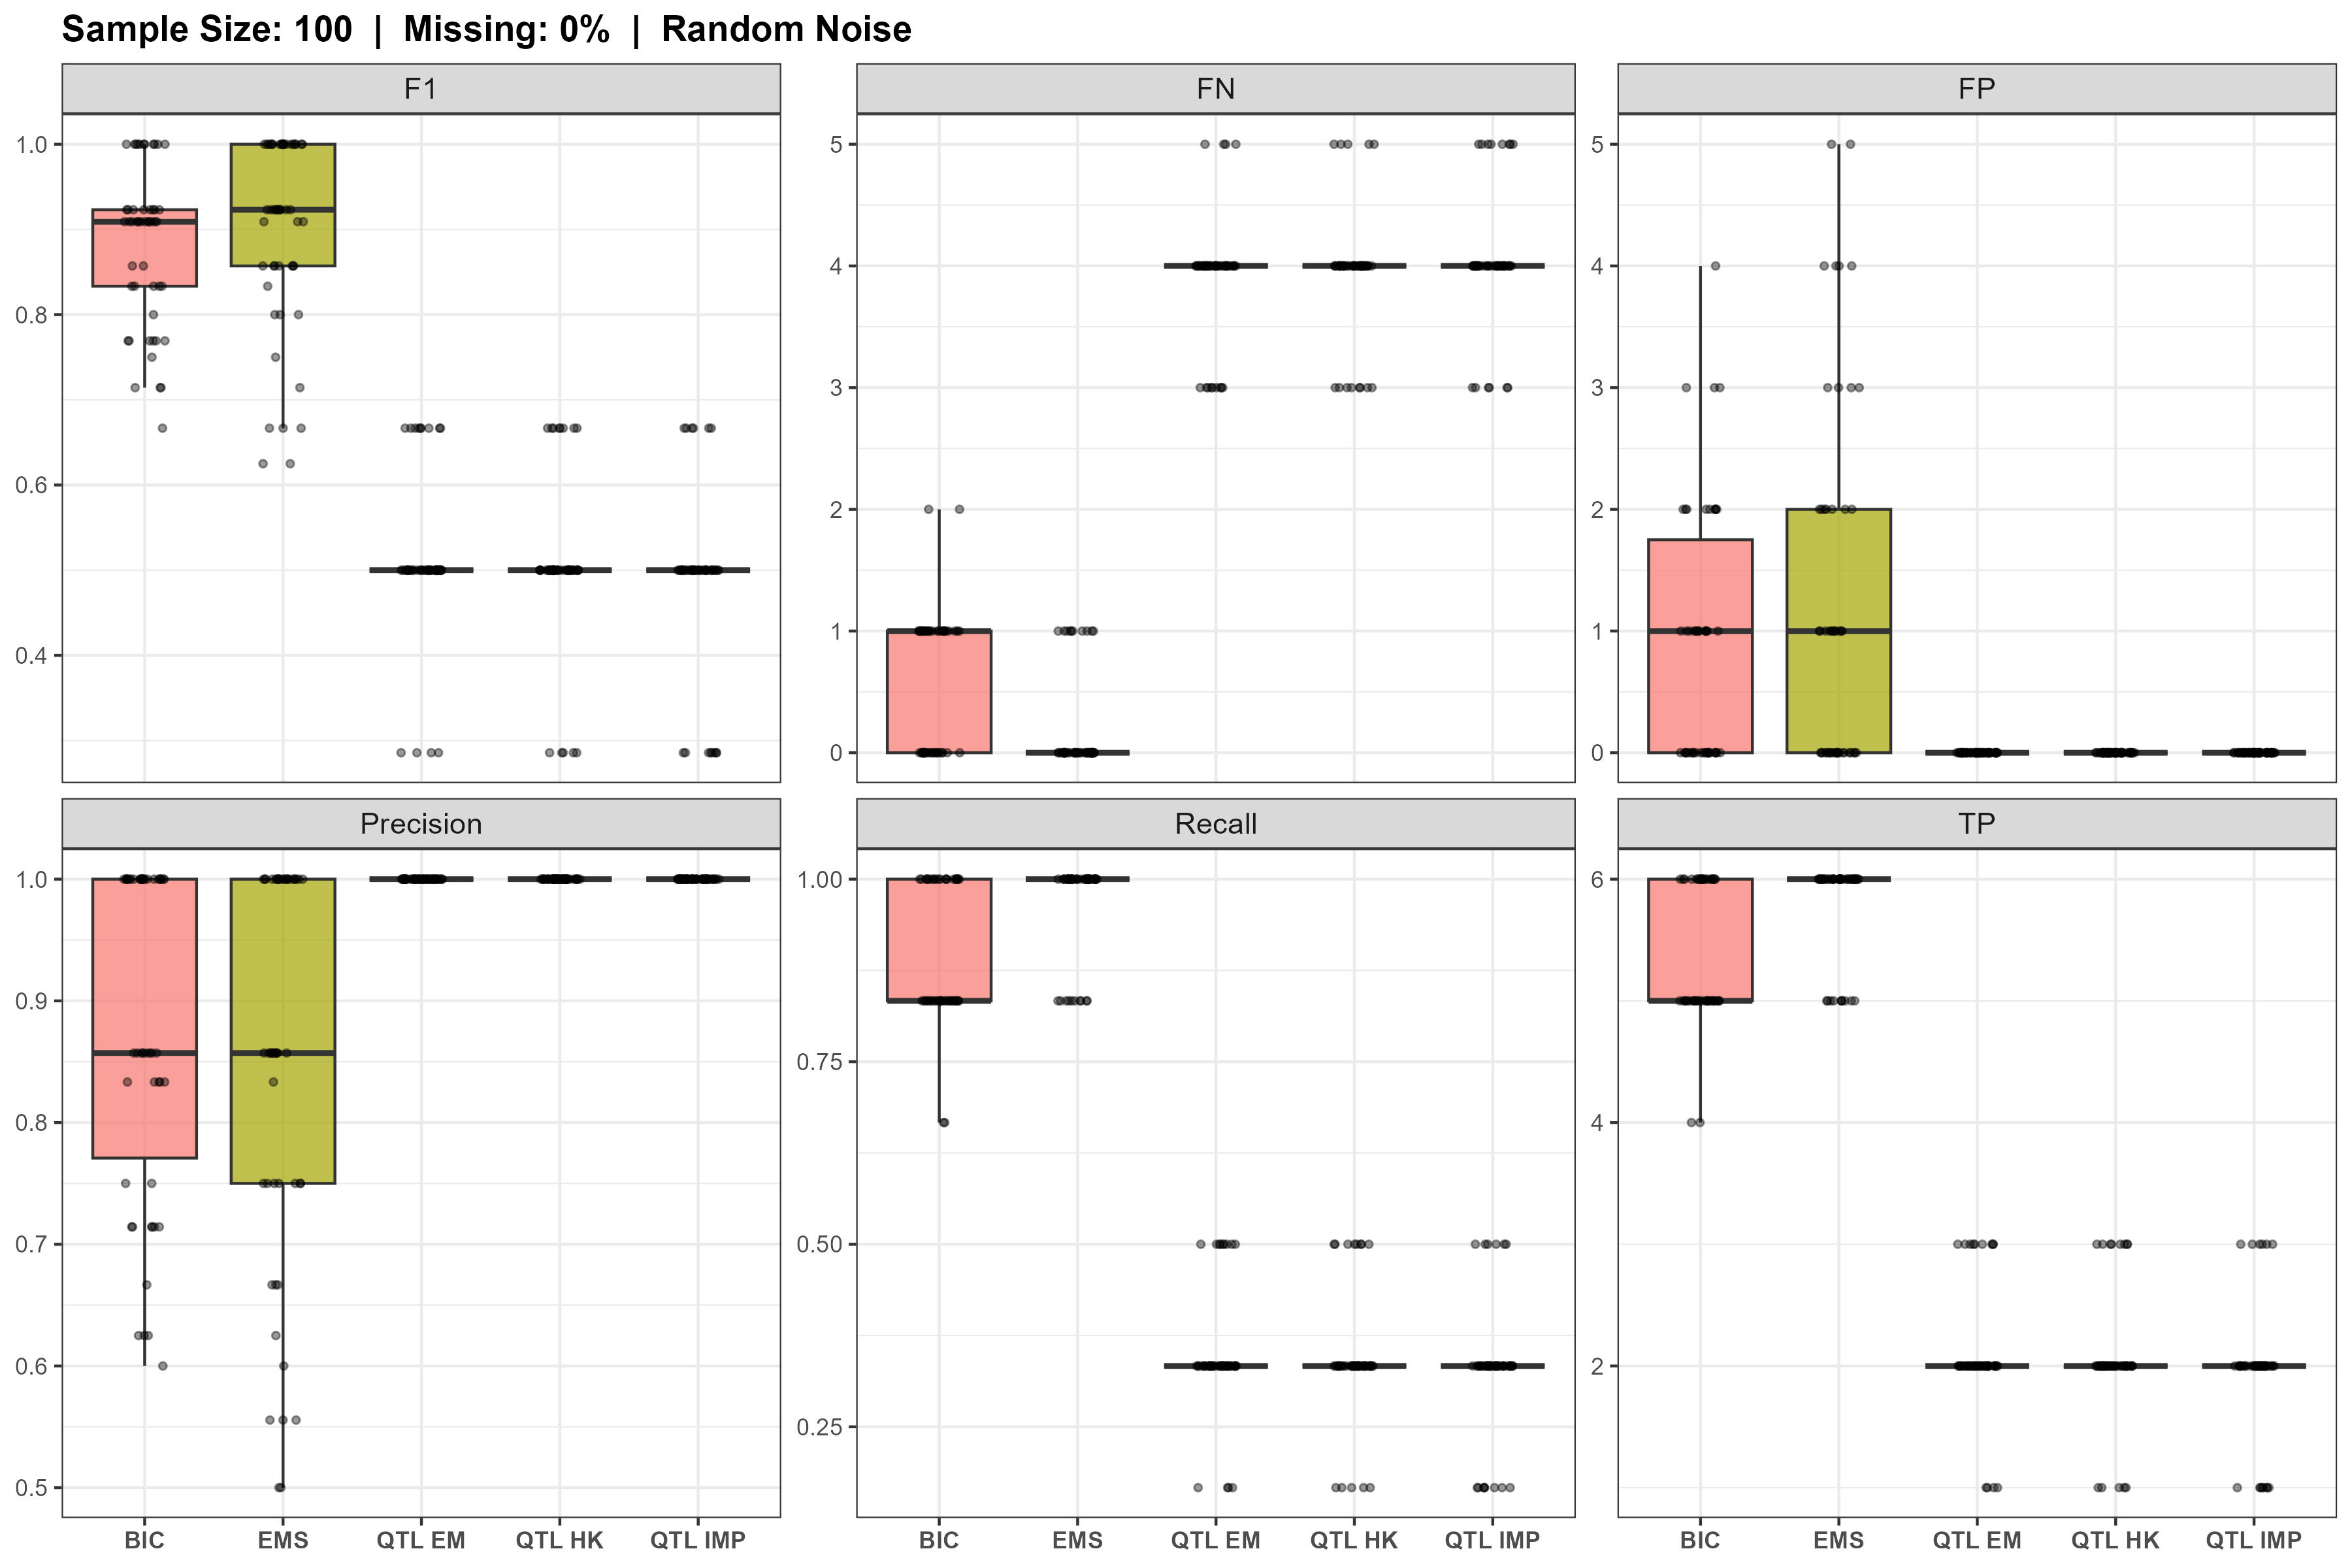
\includegraphics[width=0.95\textwidth,height=0.35\textheight,keepaspectratio]{./SuppFig_sim_n100_miss0_noise10.10.50.40.30.9.JPG}
\caption{Performance across simulation condition 8. Boxplots comparing F1, FN, FP, Precision, Recall, and TP metrics across baseline (BIC) and four alternative methods (EMS, QTL EM, QTL HK, QTL IMP) under random noise conditions with 0\% missing data (sample size: 100). Results show minimal variation across methods with complete data.}
\label{fig:sim8}
\end{figure}

\begin{figure}[H]
\centering
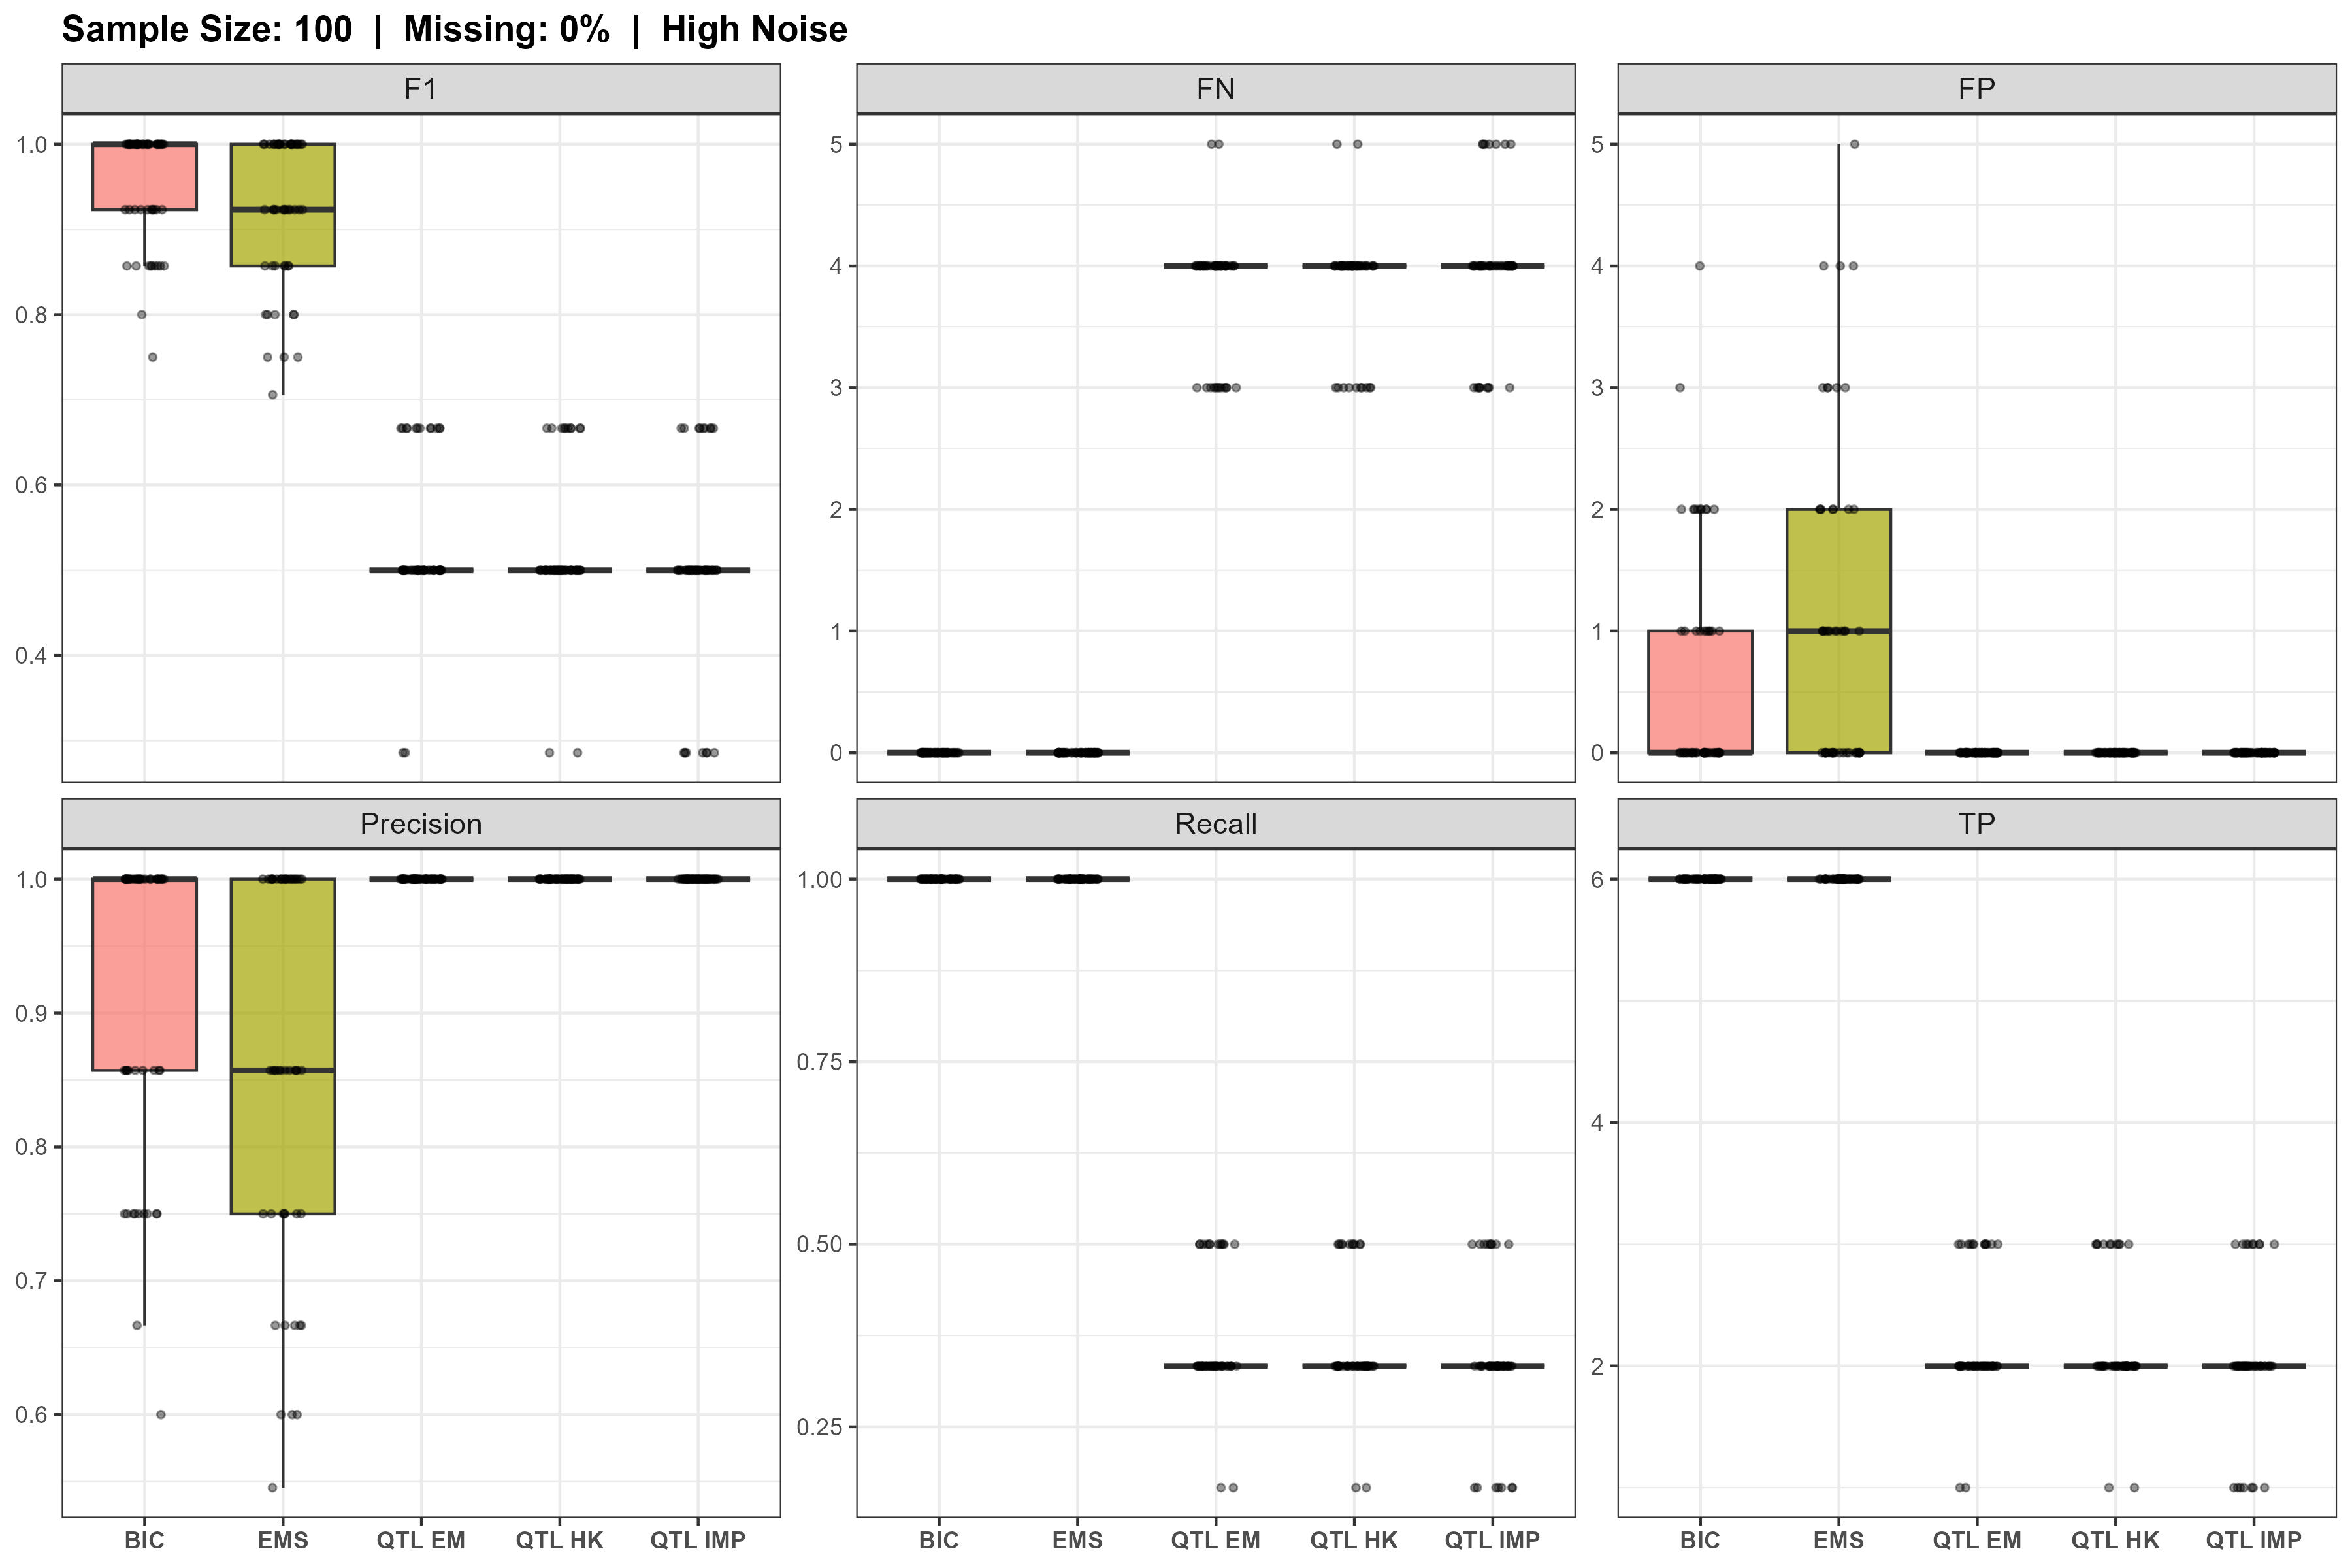
\includegraphics[width=0.95\textwidth,height=0.35\textheight,keepaspectratio]{./SuppFig_sim_n100_miss0_noise111111.JPG}
\caption{Performance across simulation condition 9. Boxplots comparing F1, FN, FP, Precision, Recall, and TP metrics across baseline (BIC) and four alternative methods (EMS, QTL EM, QTL HK, QTL IMP) under high noise conditions with 0\% missing data (sample size: 100). QTL variants show enhanced stability in high noise even without missing data complications.}
\label{fig:sim9}

\vspace{0.5cm}

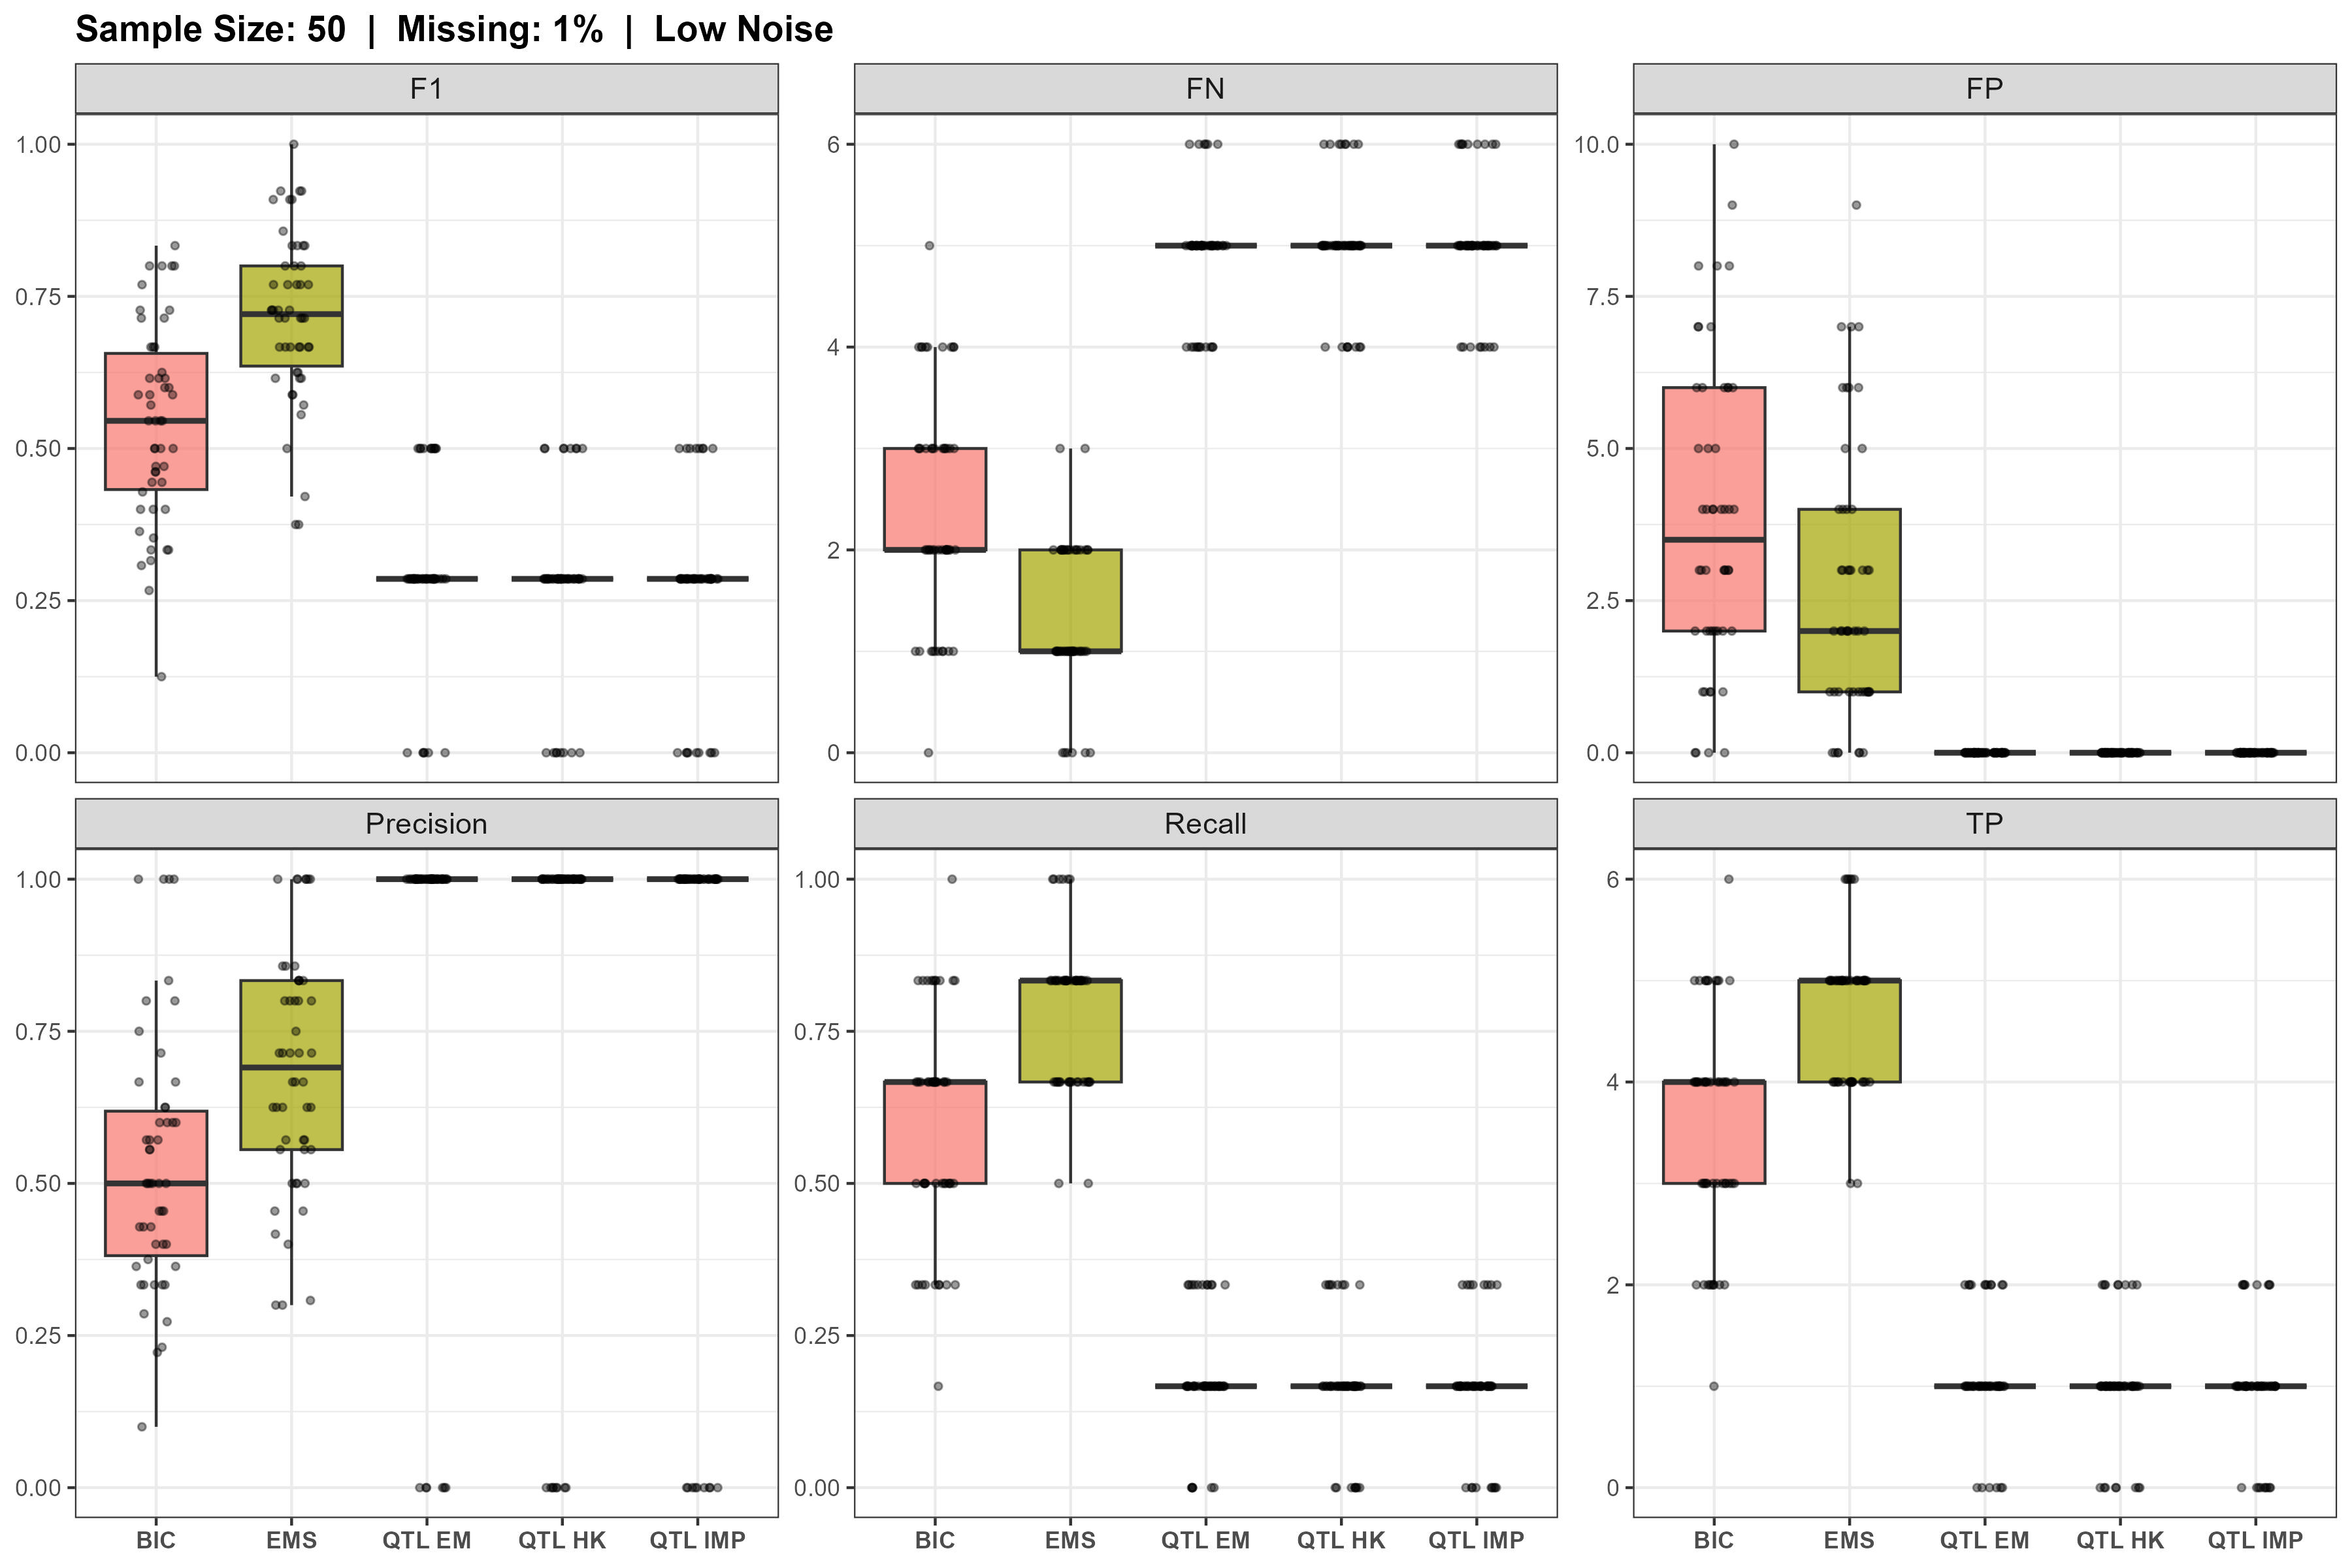
\includegraphics[width=0.95\textwidth,height=0.35\textheight,keepaspectratio]{./SuppFig_sim_n50_miss0.01_noise0.10.10.10.10.10.1.JPG}
\caption{Performance across simulation condition 10. Boxplots comparing F1, FN, FP, Precision, Recall, and TP metrics across baseline (BIC) and four alternative methods (EMS, QTL EM, QTL HK, QTL IMP) under low noise conditions with 1\% missing data (sample size: 50). Reduced sample size shows increased variability across all methods.}
\label{fig:sim10}
\end{figure}

\begin{figure}[H]
\centering
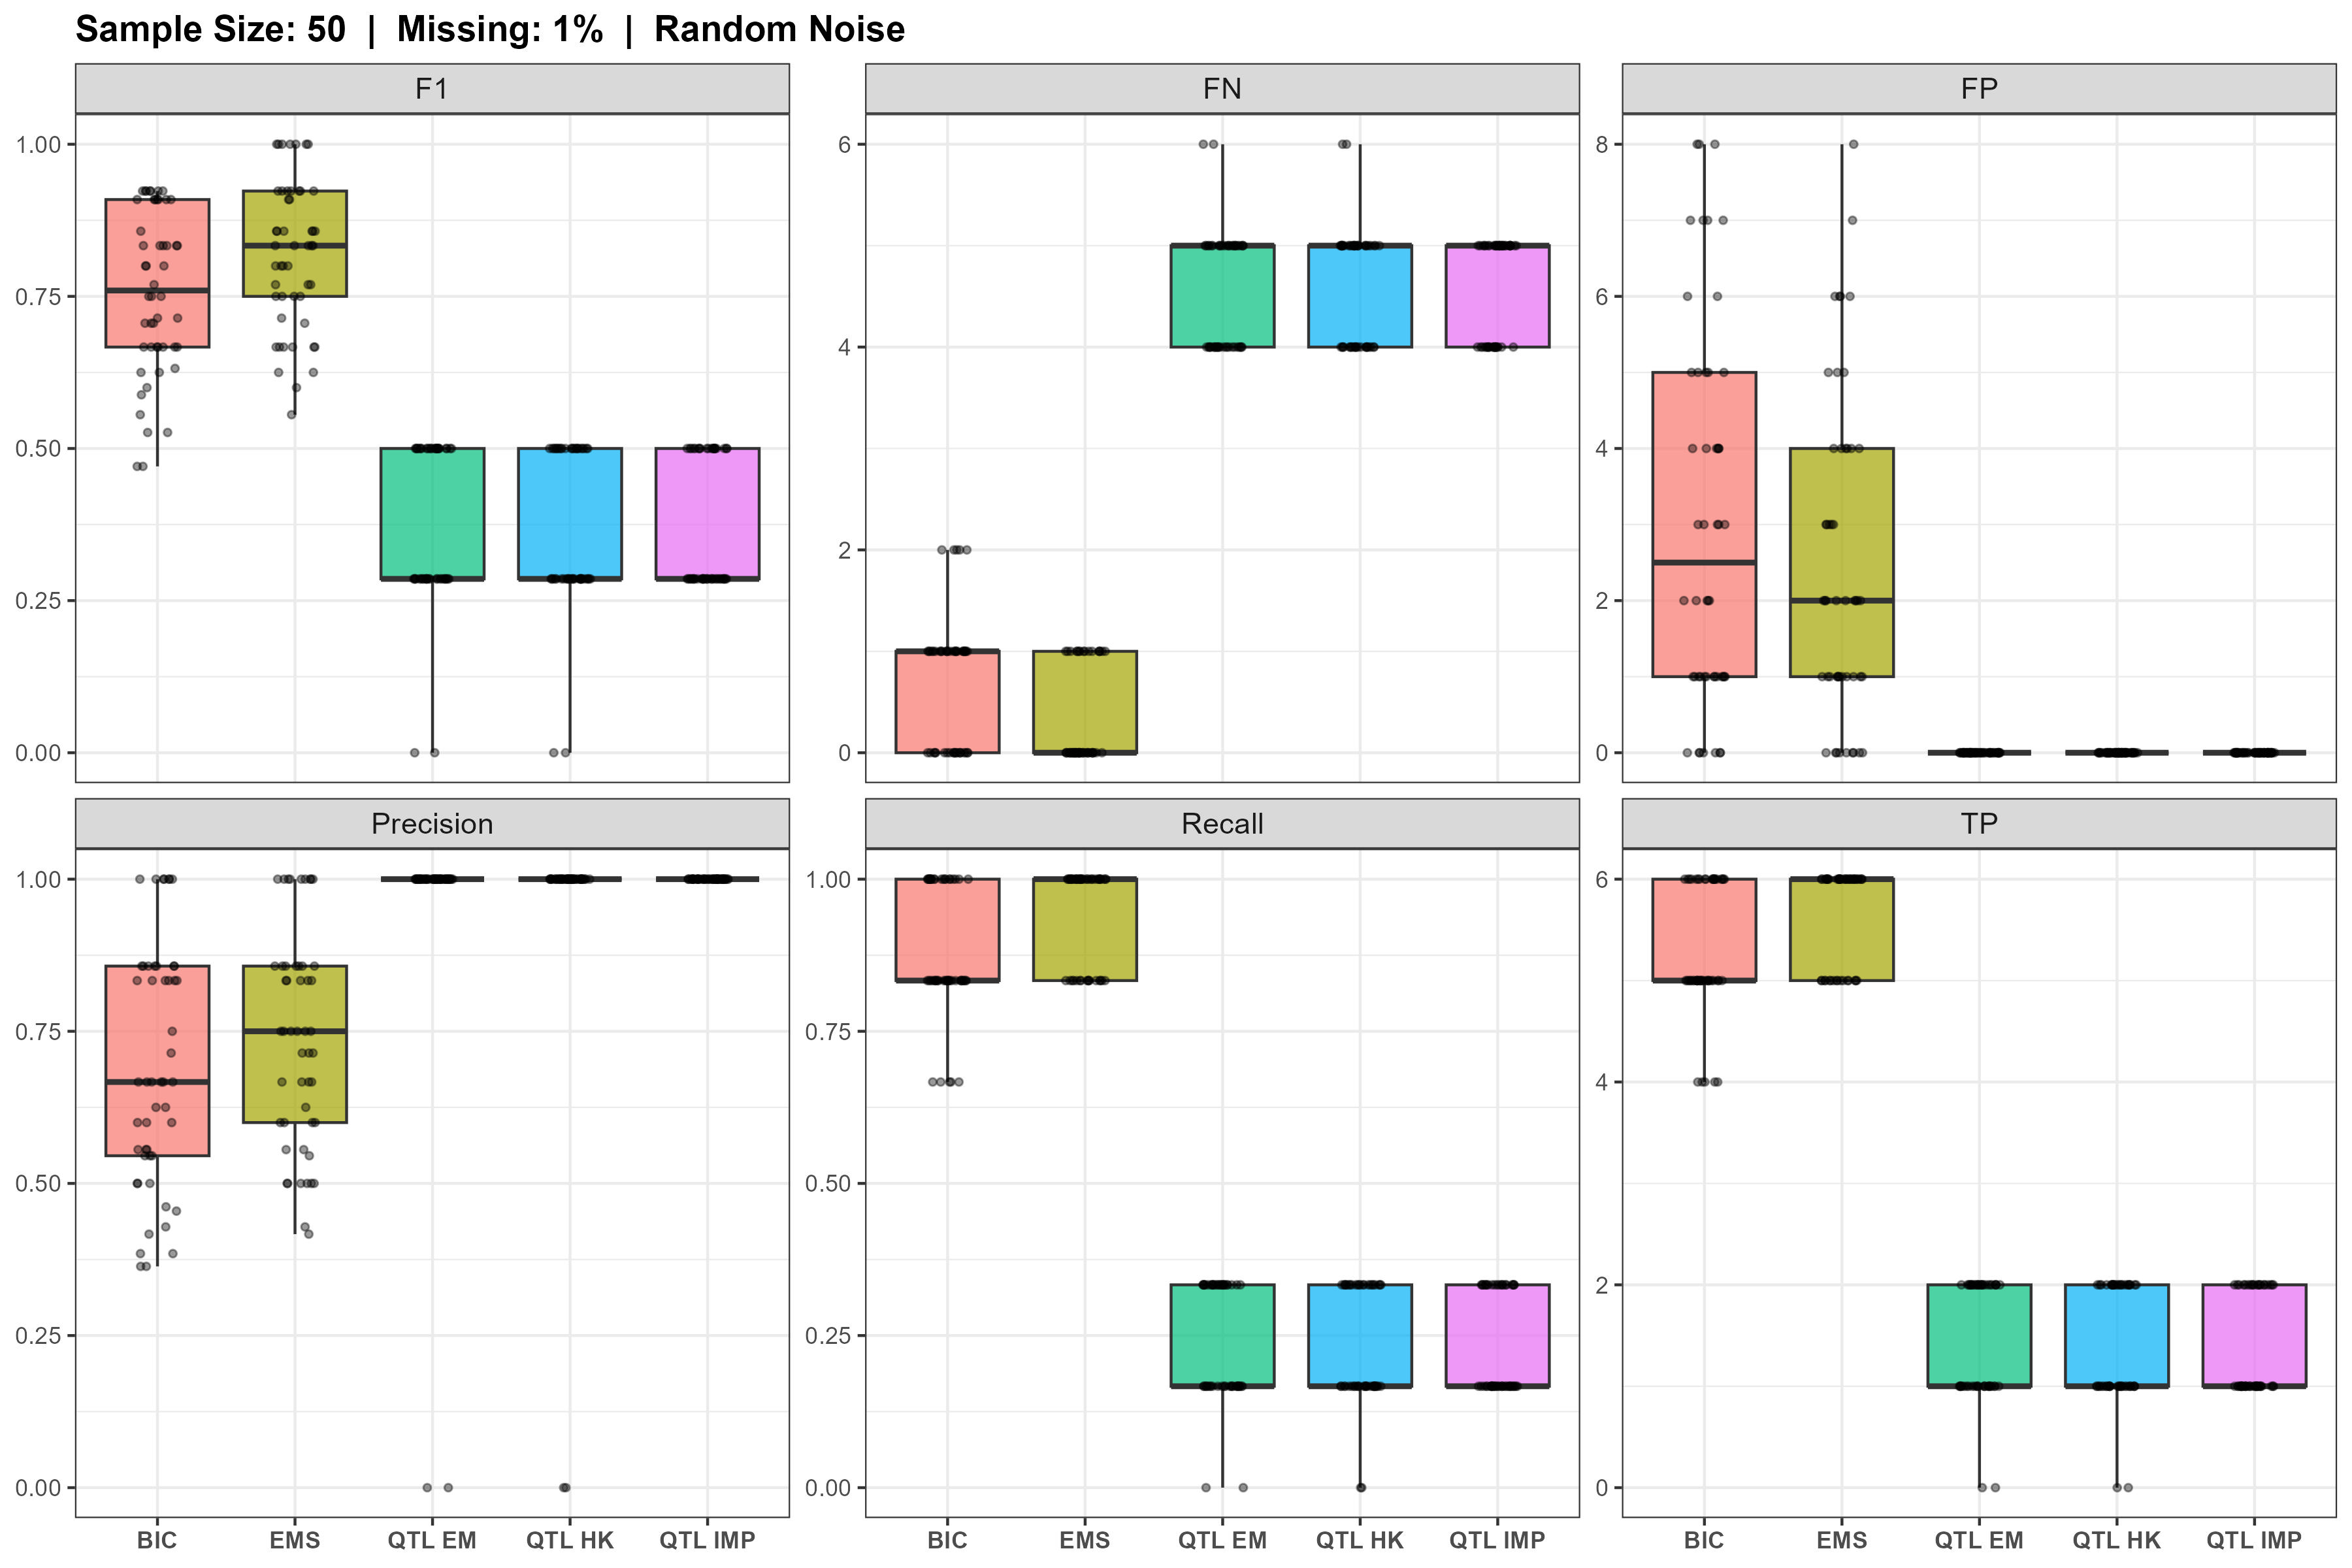
\includegraphics[width=0.95\textwidth,height=0.35\textheight,keepaspectratio]{./SuppFig_sim_n50_miss0.01_noise10.10.50.40.30.9.JPG}
\caption{Performance across simulation condition 11. Boxplots comparing F1, FN, FP, Precision, Recall, and TP metrics across baseline (BIC) and four alternative methods (EMS, QTL EM, QTL HK, QTL IMP) under random noise conditions with 1\% missing data (sample size: 50). Performance variance increases noticeably with smaller sample size.}
\label{fig:sim11}

\vspace{0.5cm}

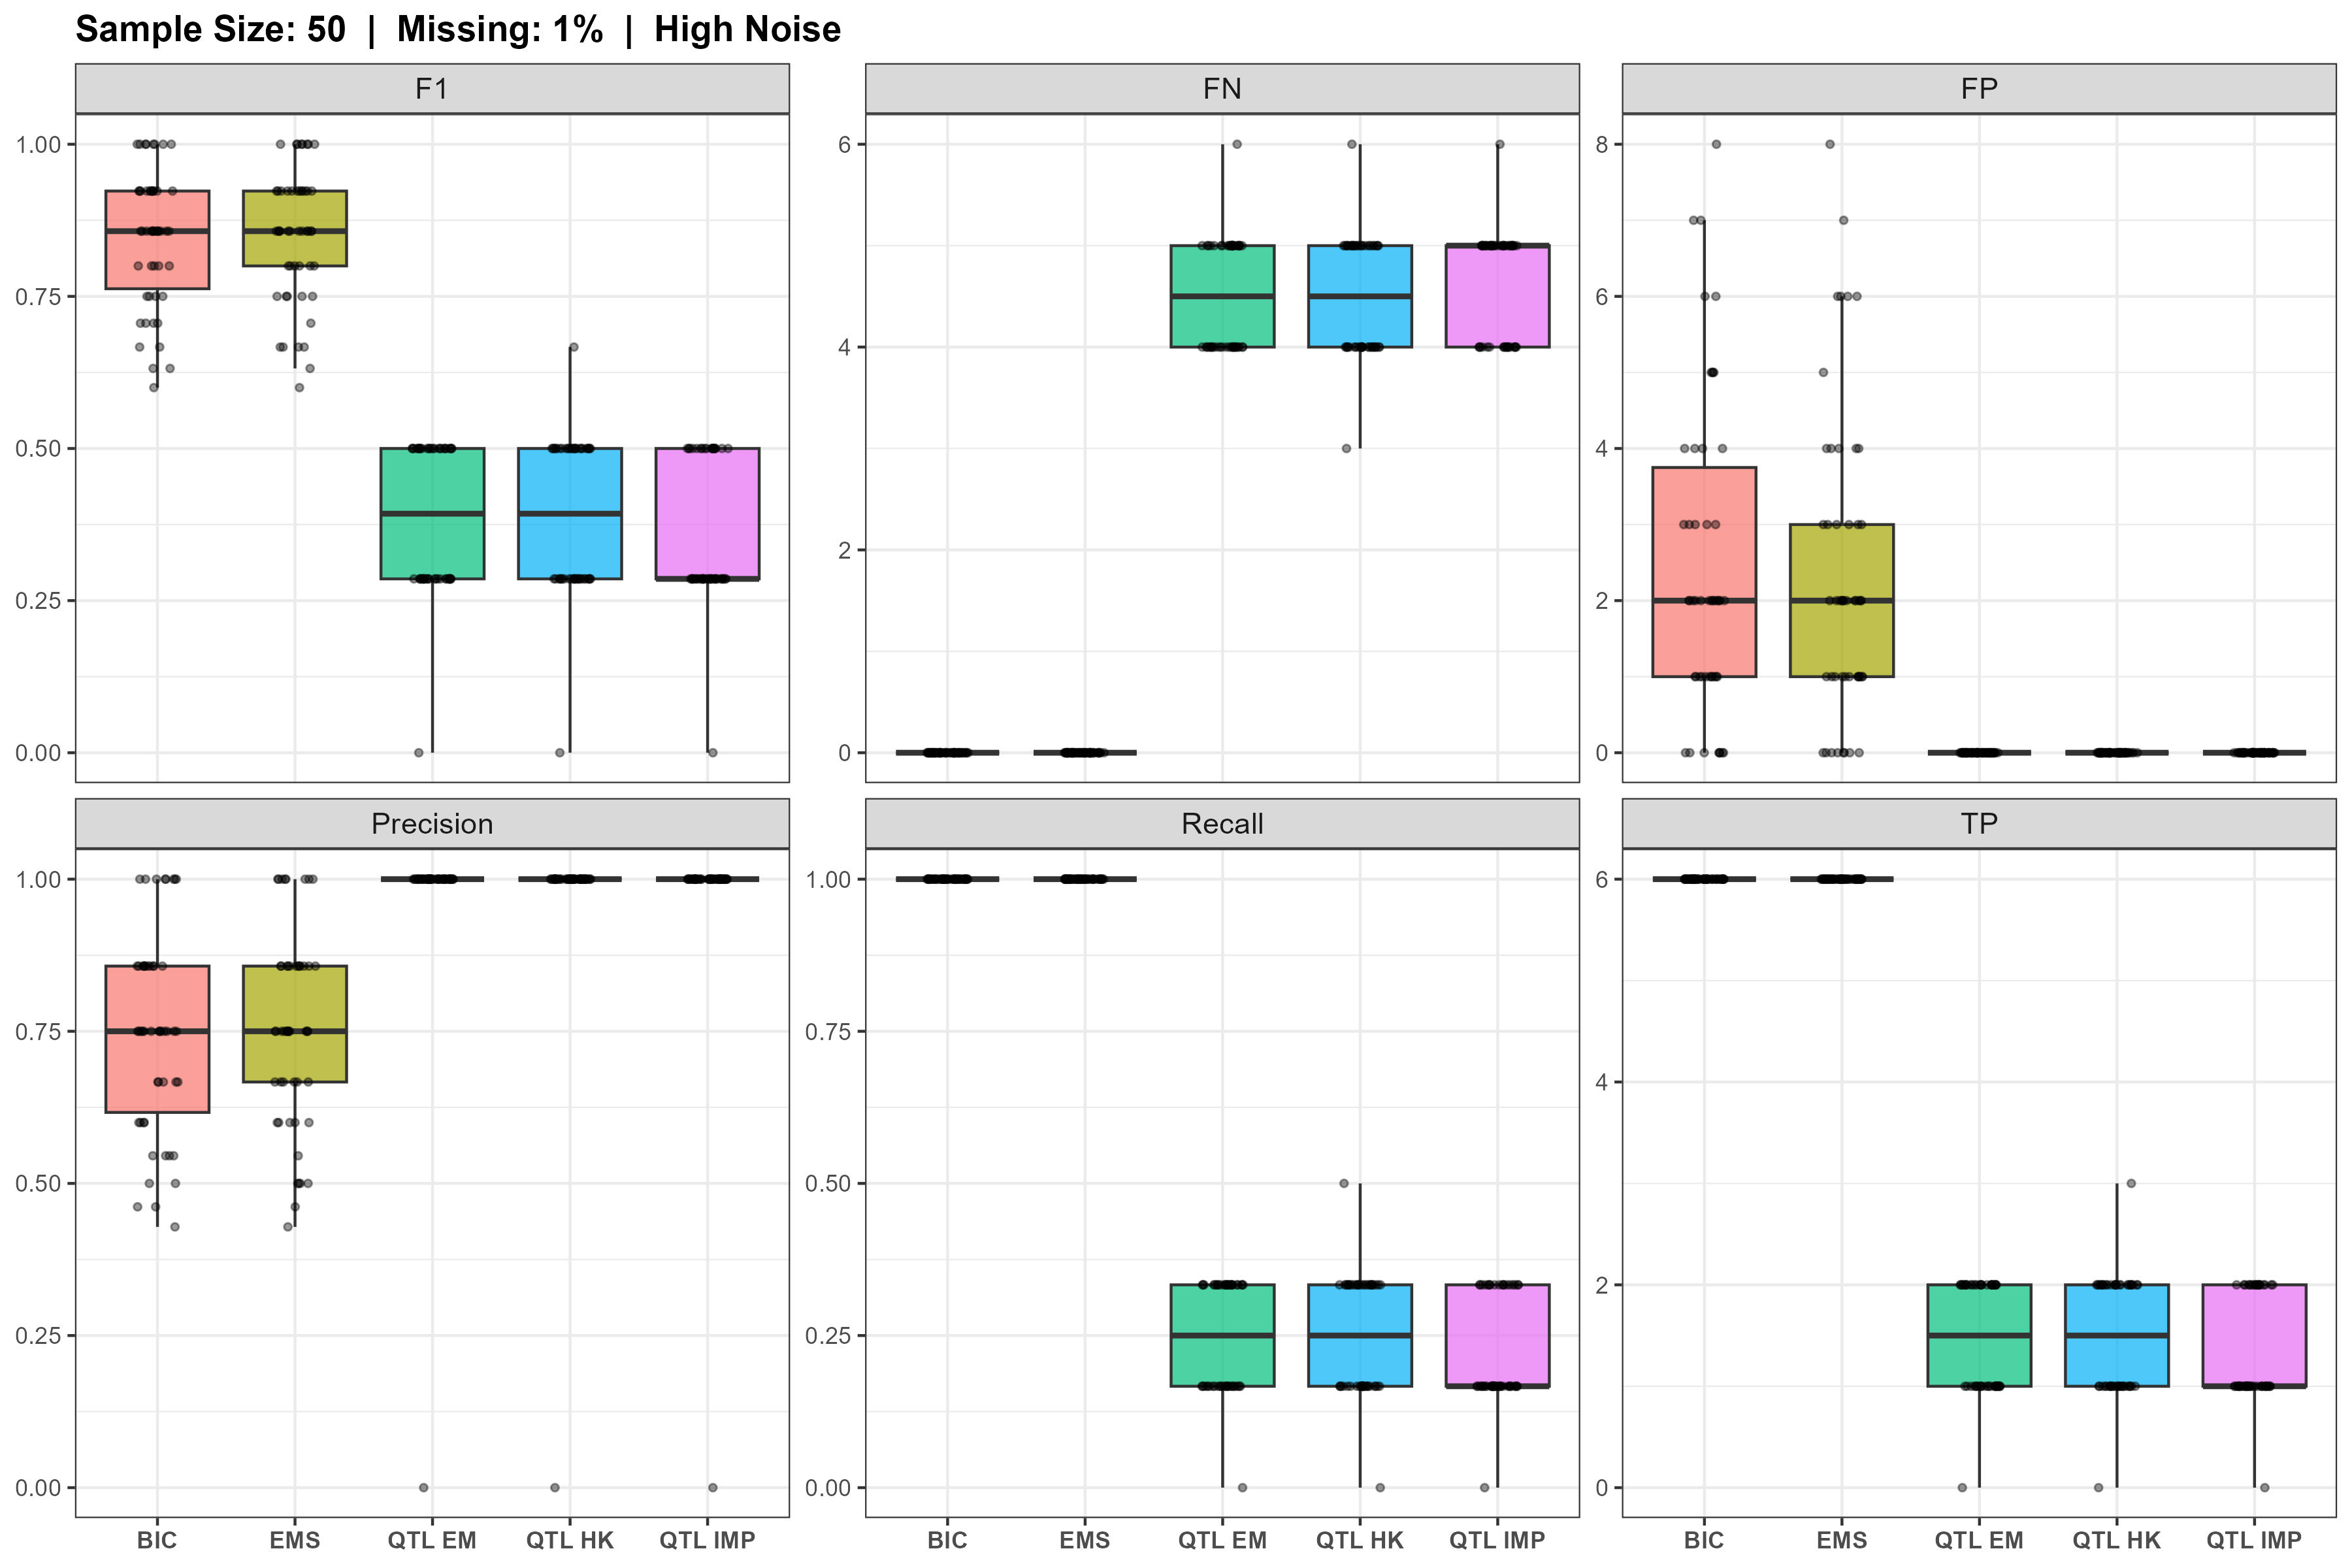
\includegraphics[width=0.95\textwidth,height=0.35\textheight,keepaspectratio]{./SuppFig_sim_n50_miss0.01_noise111111.JPG}
\caption{Performance across simulation condition 12. Boxplots comparing F1, FN, FP, Precision, Recall, and TP metrics across baseline (BIC) and four alternative methods (EMS, QTL EM, QTL HK, QTL IMP) under high noise conditions with 1\% missing data (sample size: 50). QTL HK and QTL IMP continue to outperform baseline despite sample size reduction.}
\label{fig:sim12}
\end{figure}

\begin{figure}[H]
\centering
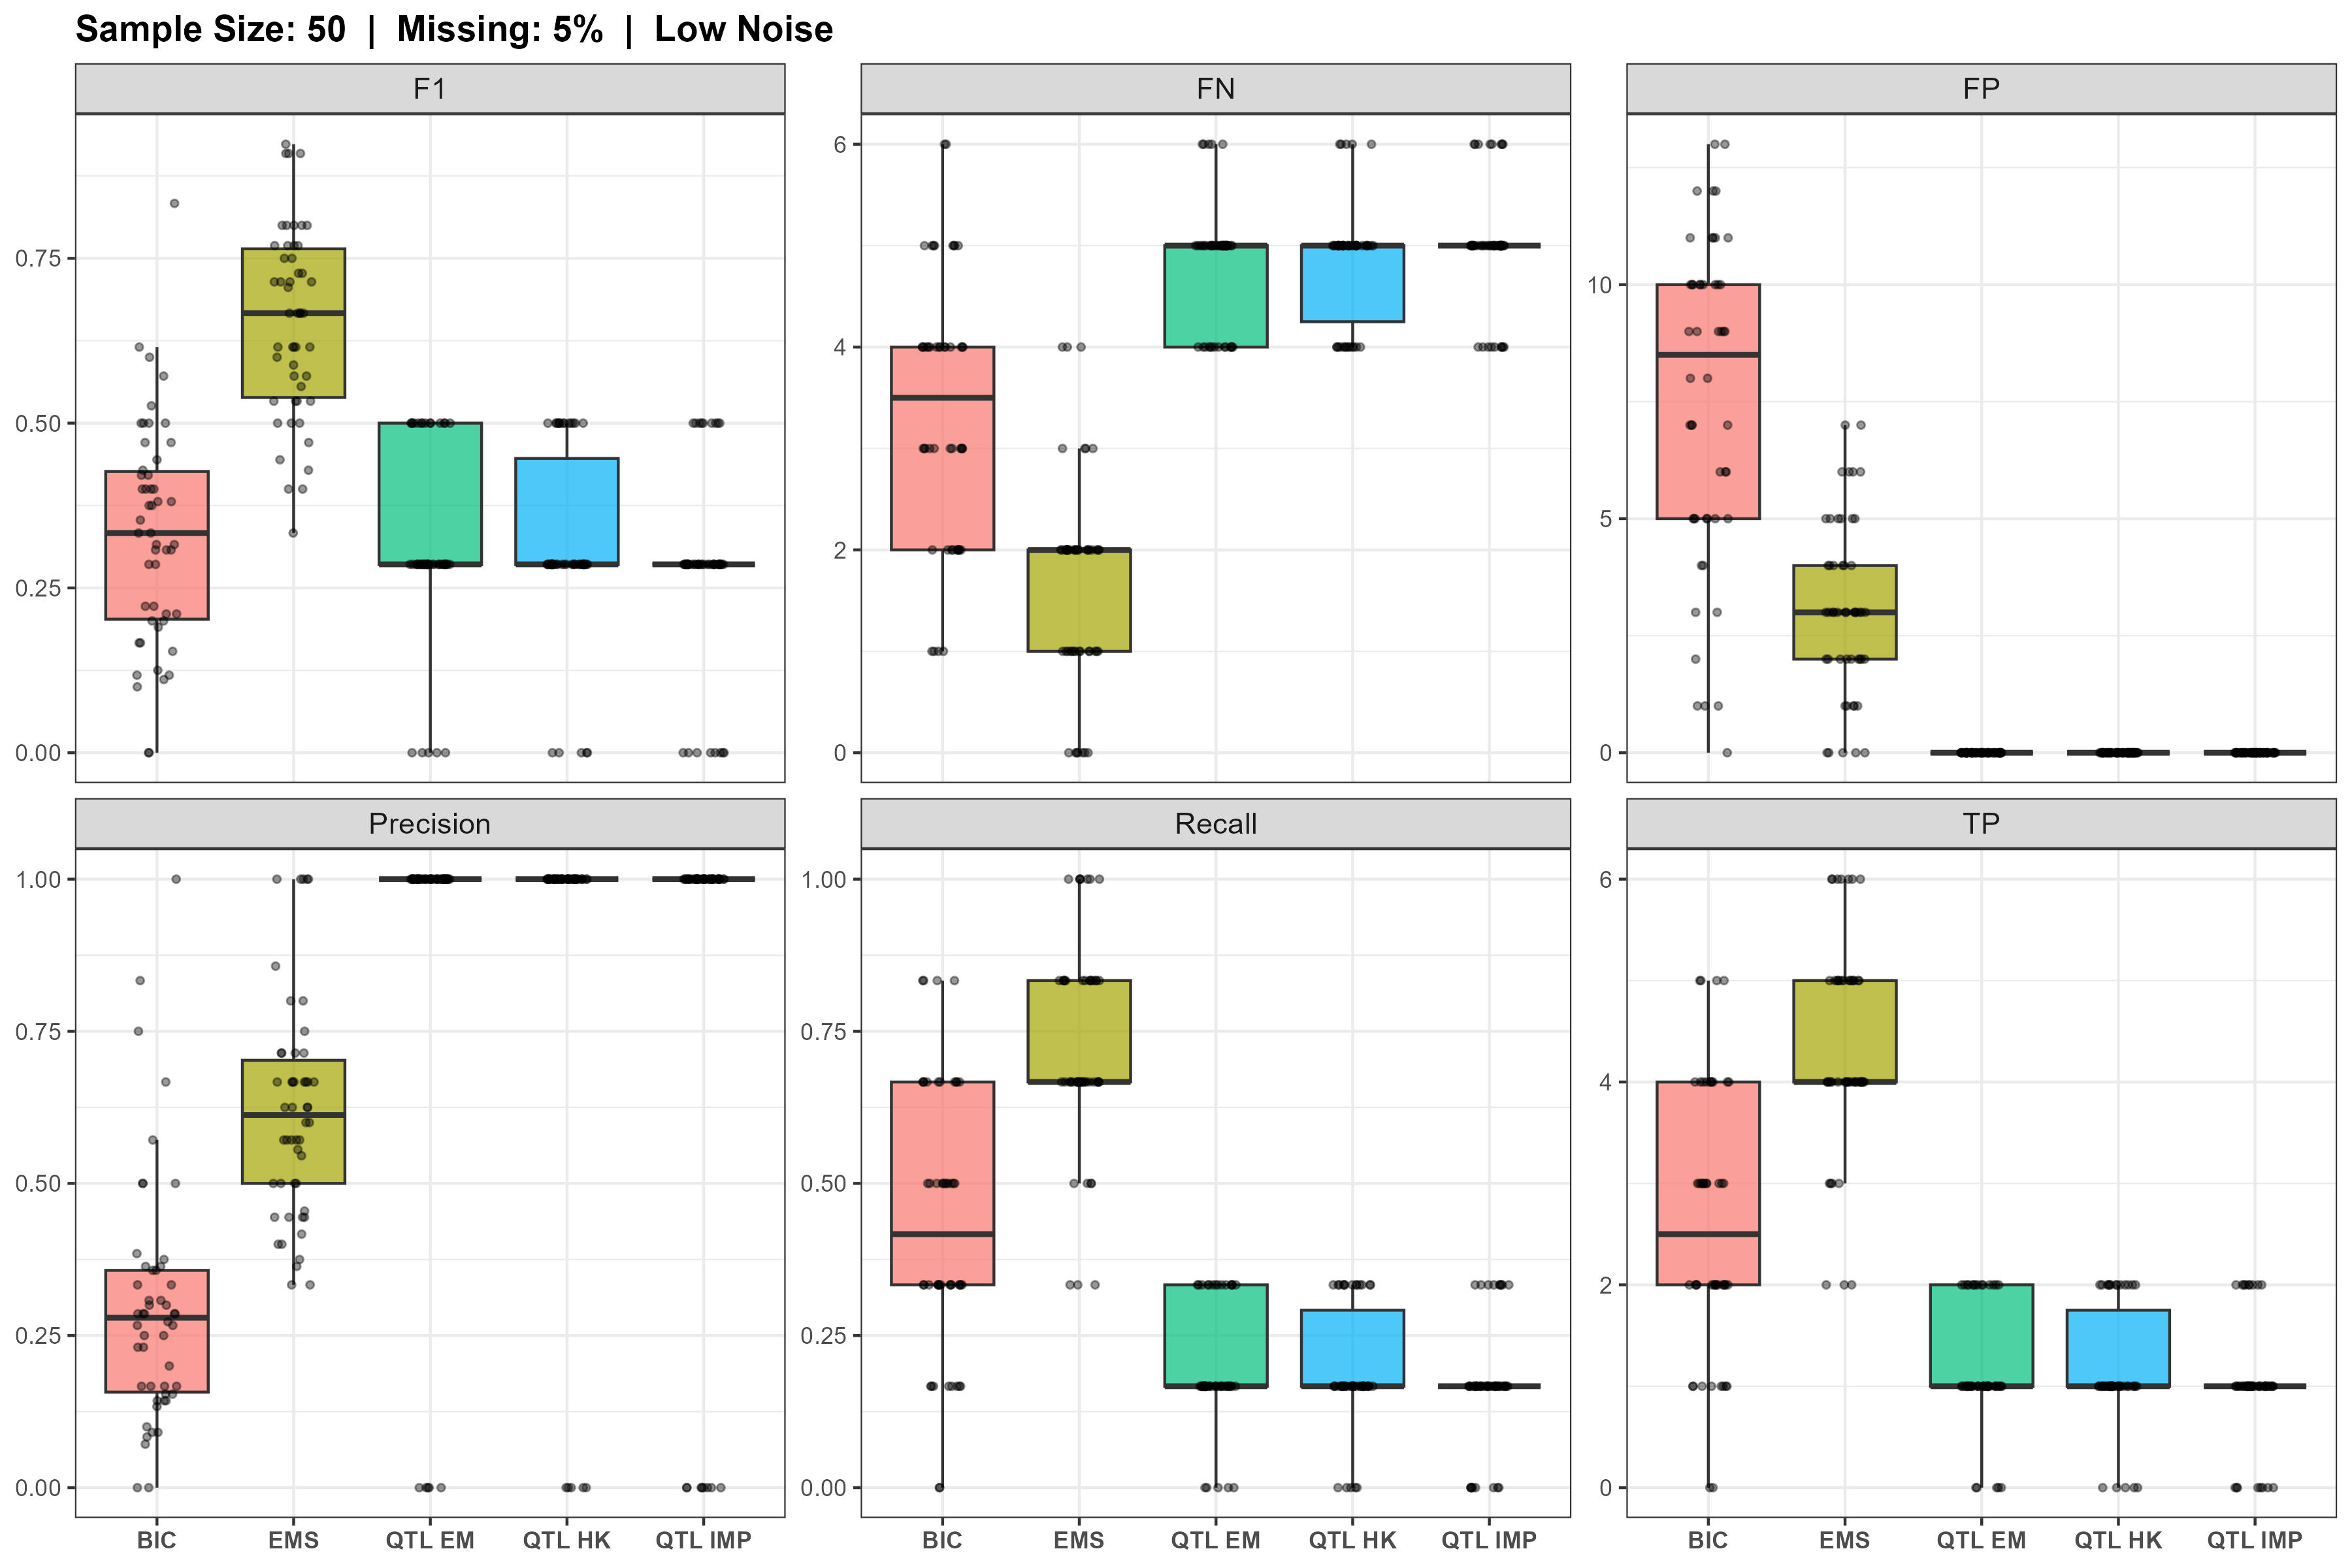
\includegraphics[width=0.95\textwidth,height=0.35\textheight,keepaspectratio]{./SuppFig_sim_n50_miss0.05_noise0.10.10.10.10.10.1.JPG}
\caption{Performance across simulation condition 13. Boxplots comparing F1, FN, FP, Precision, Recall, and TP metrics across baseline (BIC) and four alternative methods (EMS, QTL EM, QTL HK, QTL IMP) under low noise conditions with 5\% missing data (sample size: 50). Increased missingness combined with smaller sample yields greater performance dispersion.}
\label{fig:sim13}

\vspace{0.5cm}

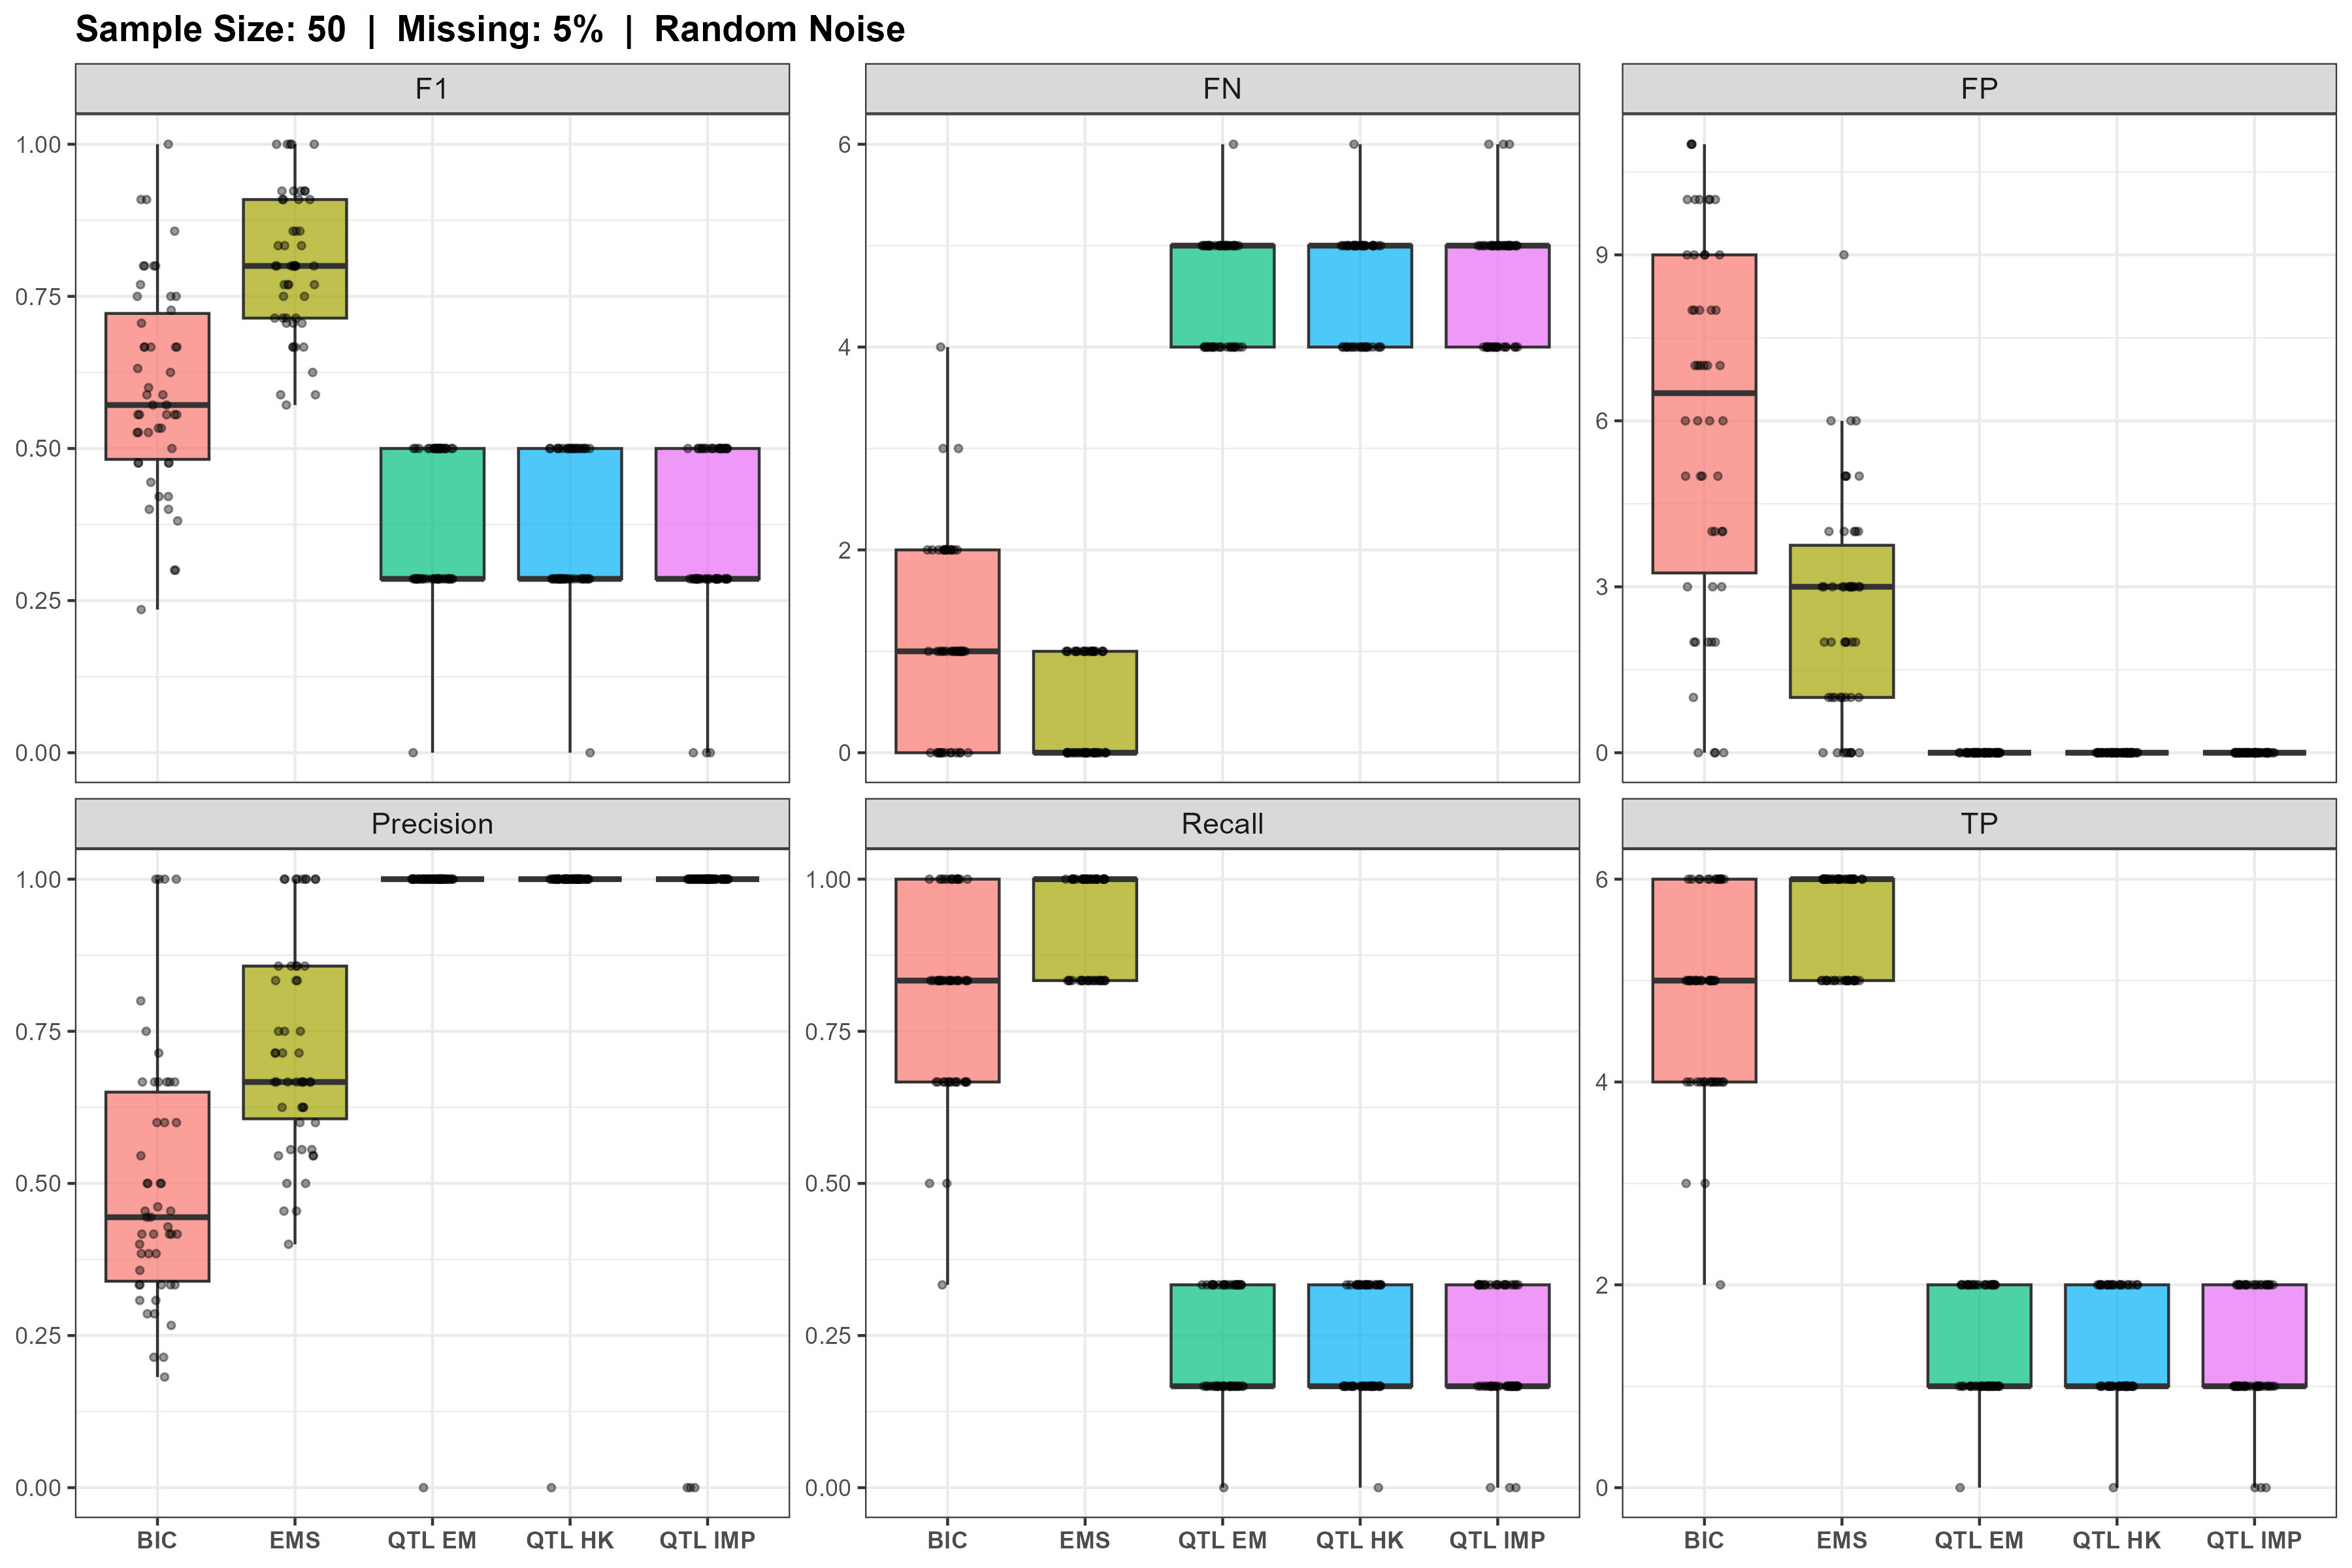
\includegraphics[width=0.95\textwidth,height=0.35\textheight,keepaspectratio]{./SuppFig_sim_n50_miss0.05_noise10.10.50.40.30.9.JPG}
\caption{Performance across simulation condition 14. Boxplots comparing F1, FN, FP, Precision, Recall, and TP metrics across baseline (BIC) and four alternative methods (EMS, QTL EM, QTL HK, QTL IMP) under random noise conditions with 5\% missing data (sample size: 50). EMS demonstrates more consistent behavior under these combined constraints.}
\label{fig:sim14}
\end{figure}

\begin{figure}[H]
\centering
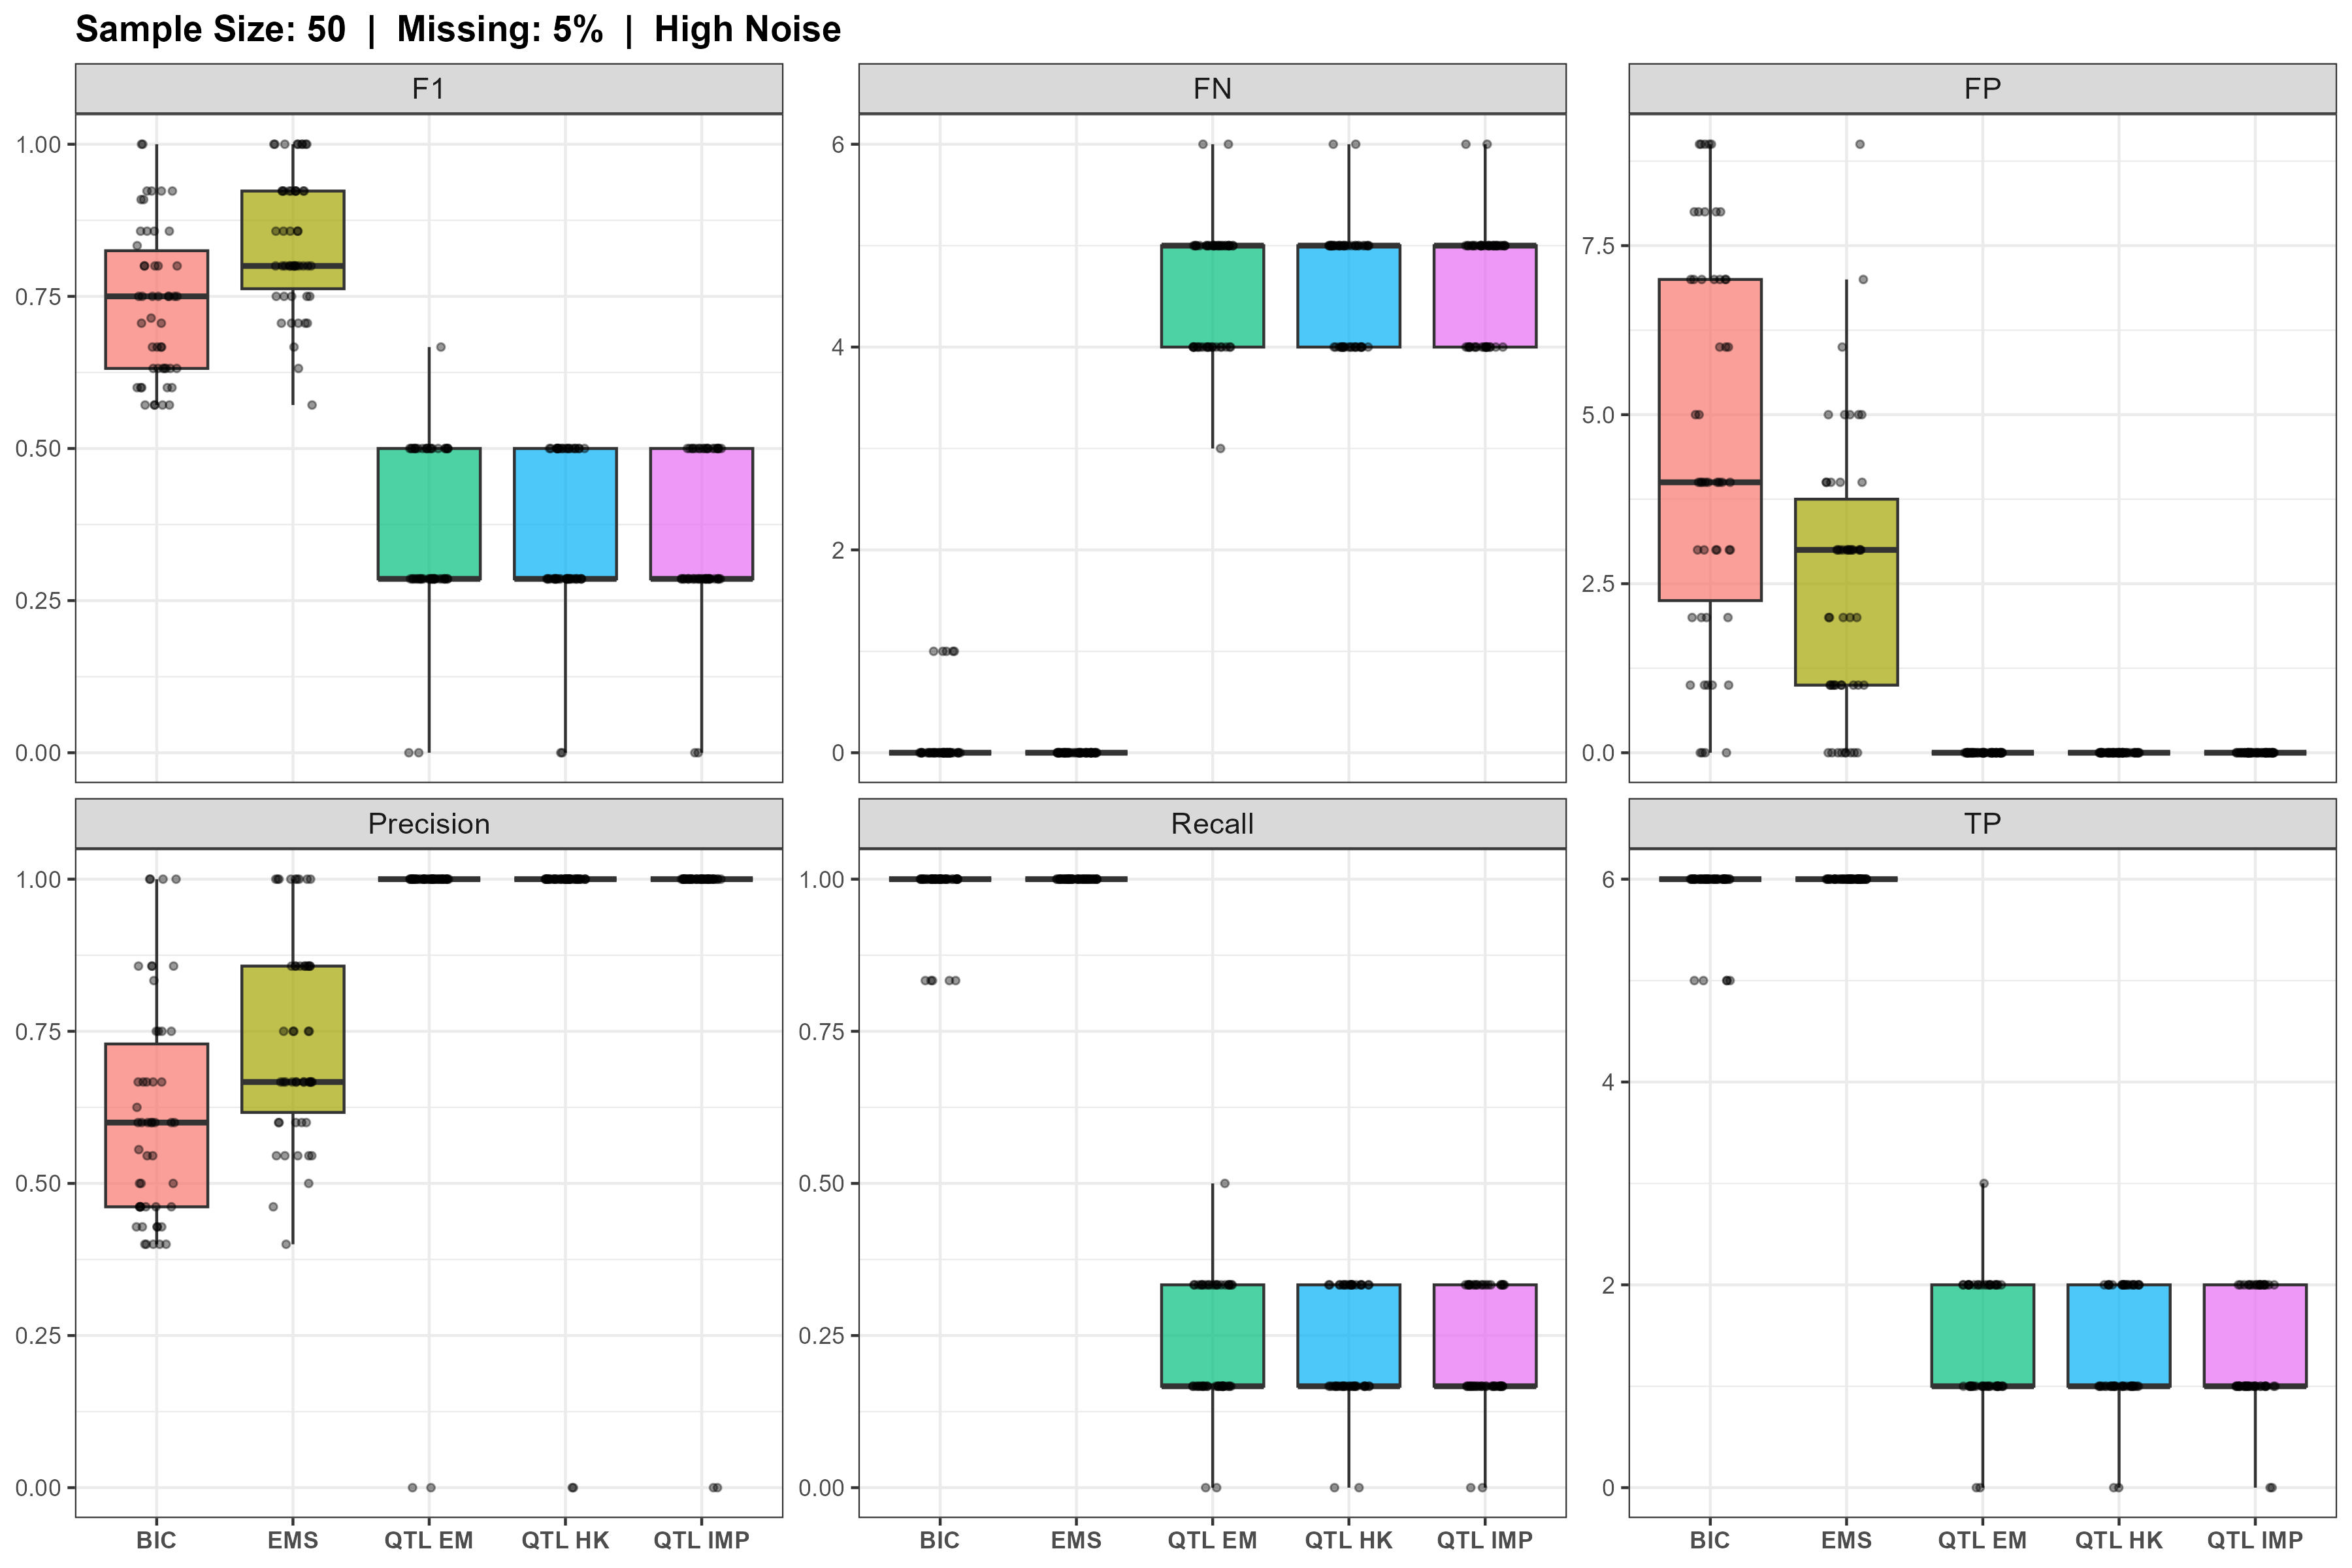
\includegraphics[width=0.95\textwidth,height=0.35\textheight,keepaspectratio]{./SuppFig_sim_n50_miss0.05_noise111111.JPG}
\caption{Performance across simulation condition 15. Boxplots comparing F1, FN, FP, Precision, Recall, and TP metrics across baseline (BIC) and four alternative methods (EMS, QTL EM, QTL HK, QTL IMP) under high noise conditions with 5\% missing data (sample size: 50). QTL variants maintain advantages even under worst-case data conditions with limited sample size.}
\label{fig:sim15}

\vspace{0.5cm}

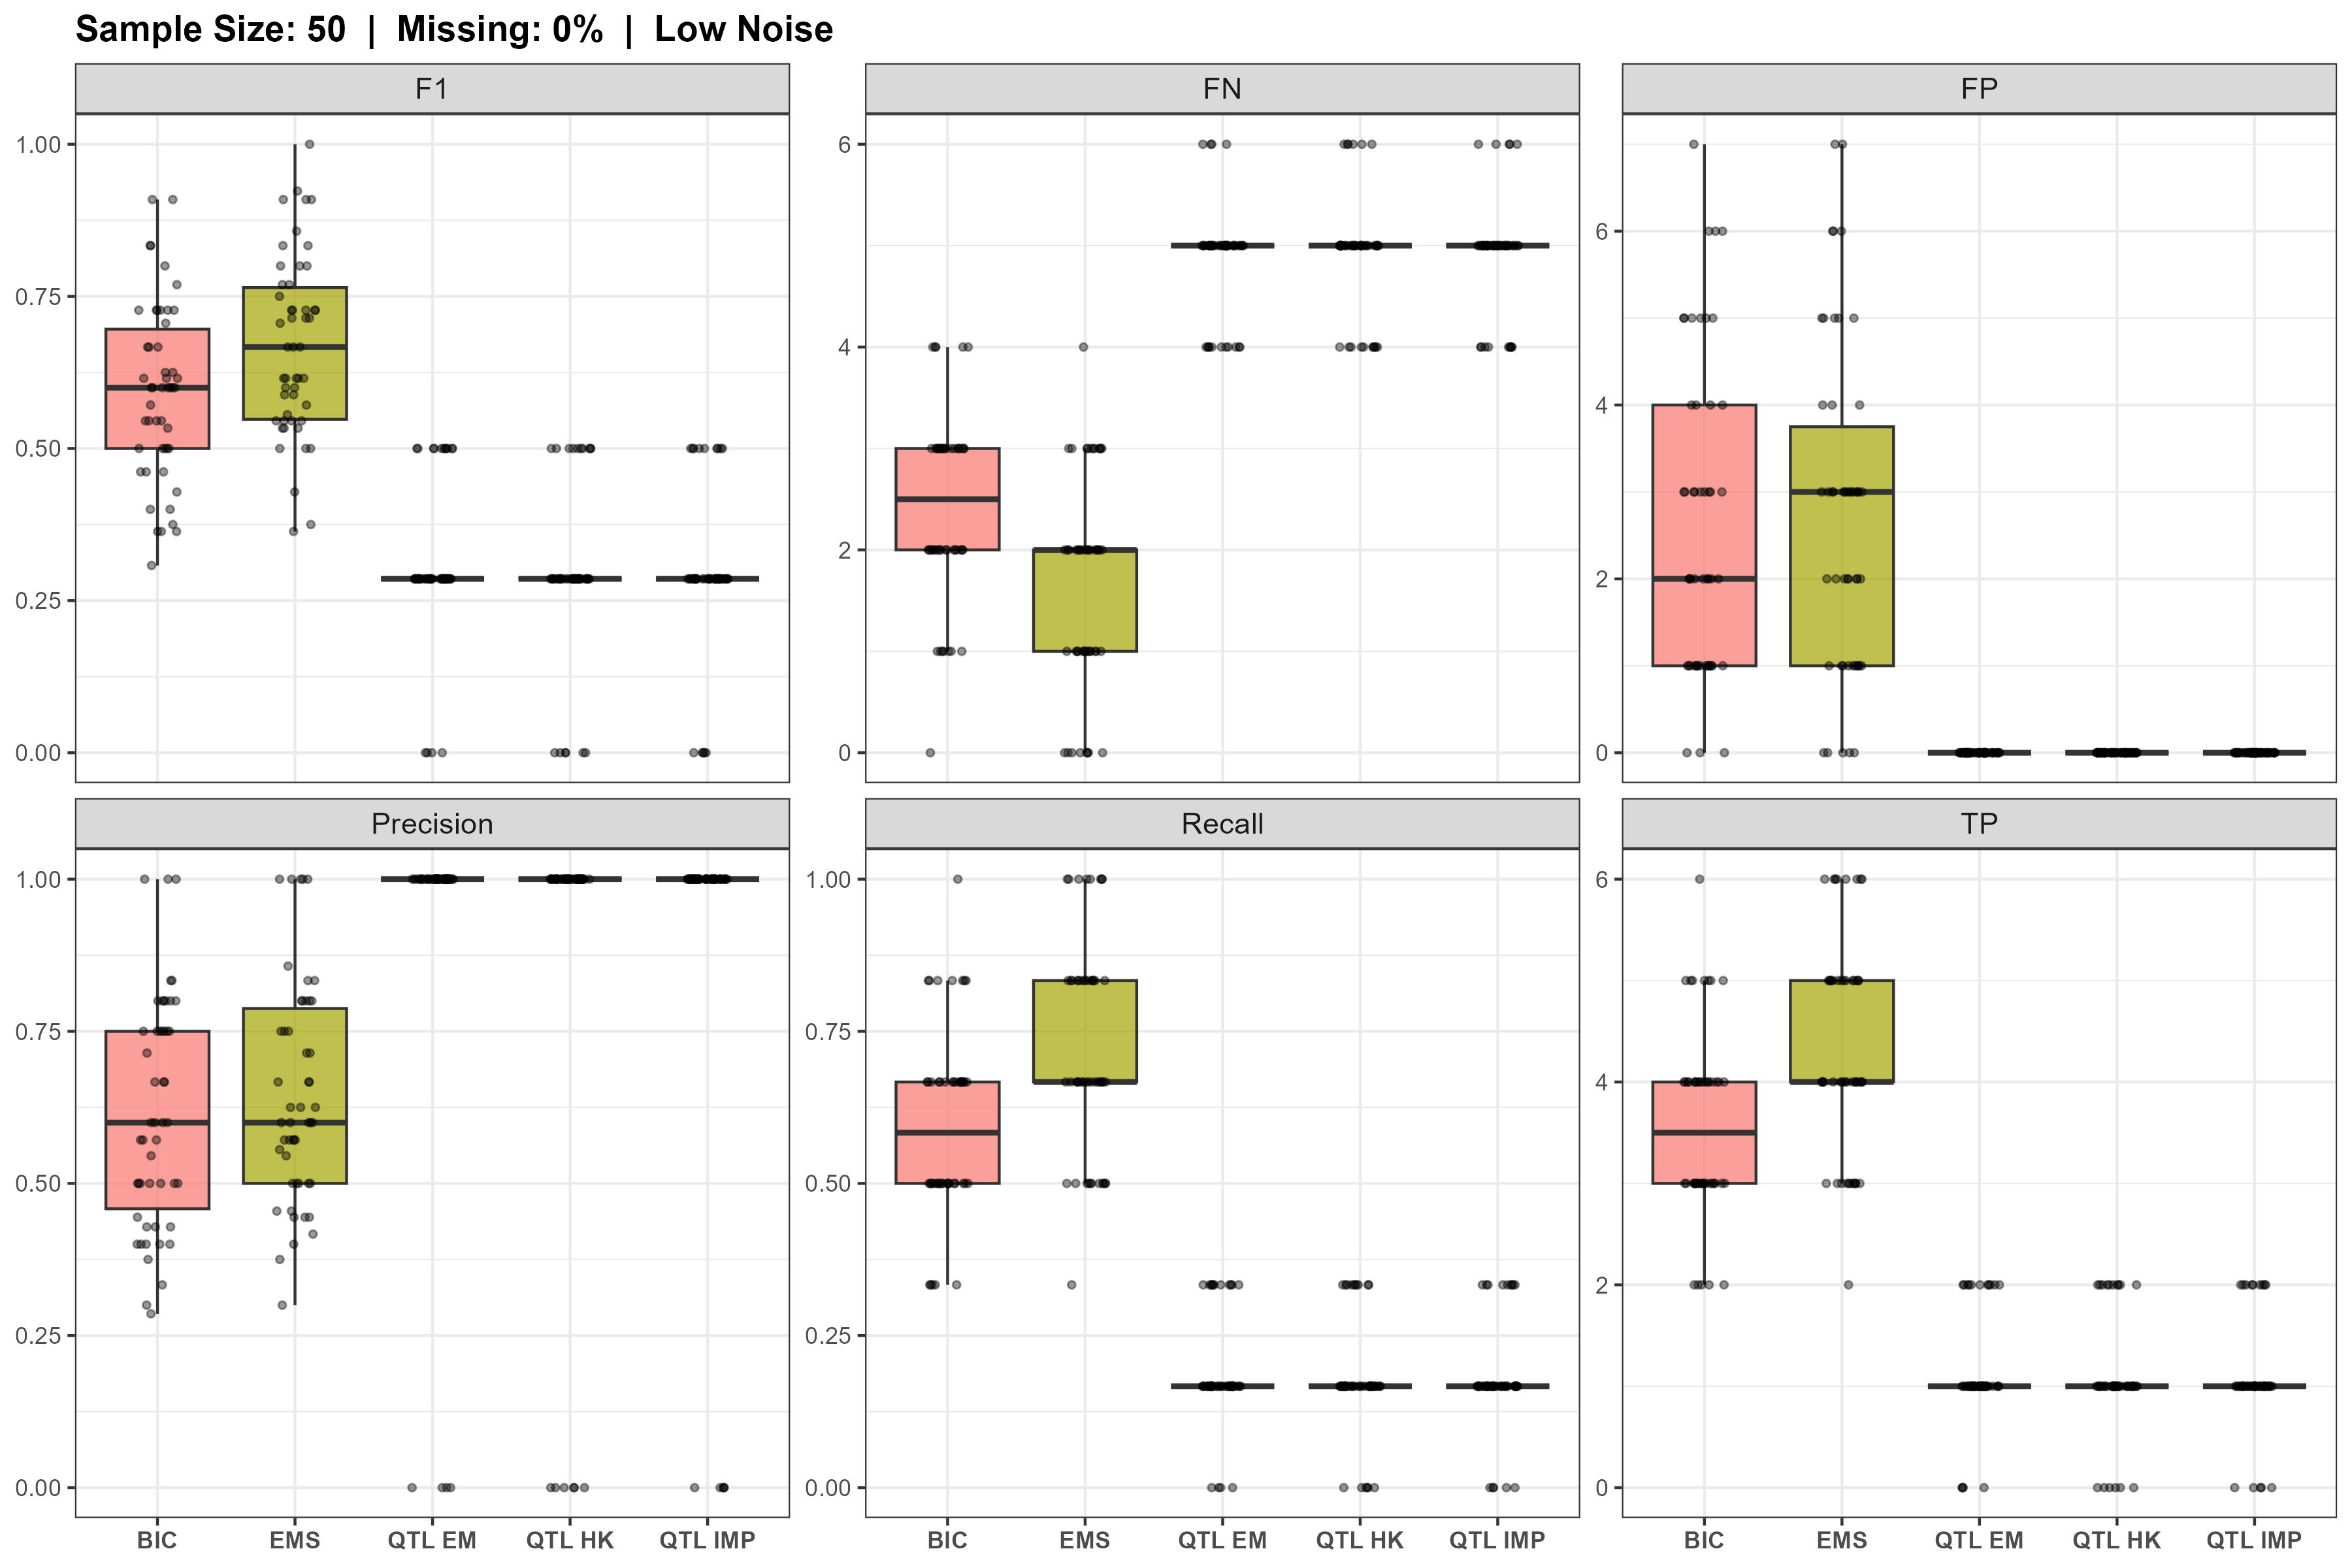
\includegraphics[width=0.95\textwidth,height=0.35\textheight,keepaspectratio]{./SuppFig_sim_n50_miss0_noise0.10.10.10.10.10.1.JPG}
\caption{Performance across simulation condition 16. Boxplots comparing F1, FN, FP, Precision, Recall, and TP metrics across baseline (BIC) and four alternative methods (EMS, QTL EM, QTL HK, QTL IMP) under low noise conditions with 0\% missing data (sample size: 50). Minimal missing data reduces variability despite smaller sample size.}
\label{fig:sim16}
\end{figure}

\begin{figure}[H]
\centering
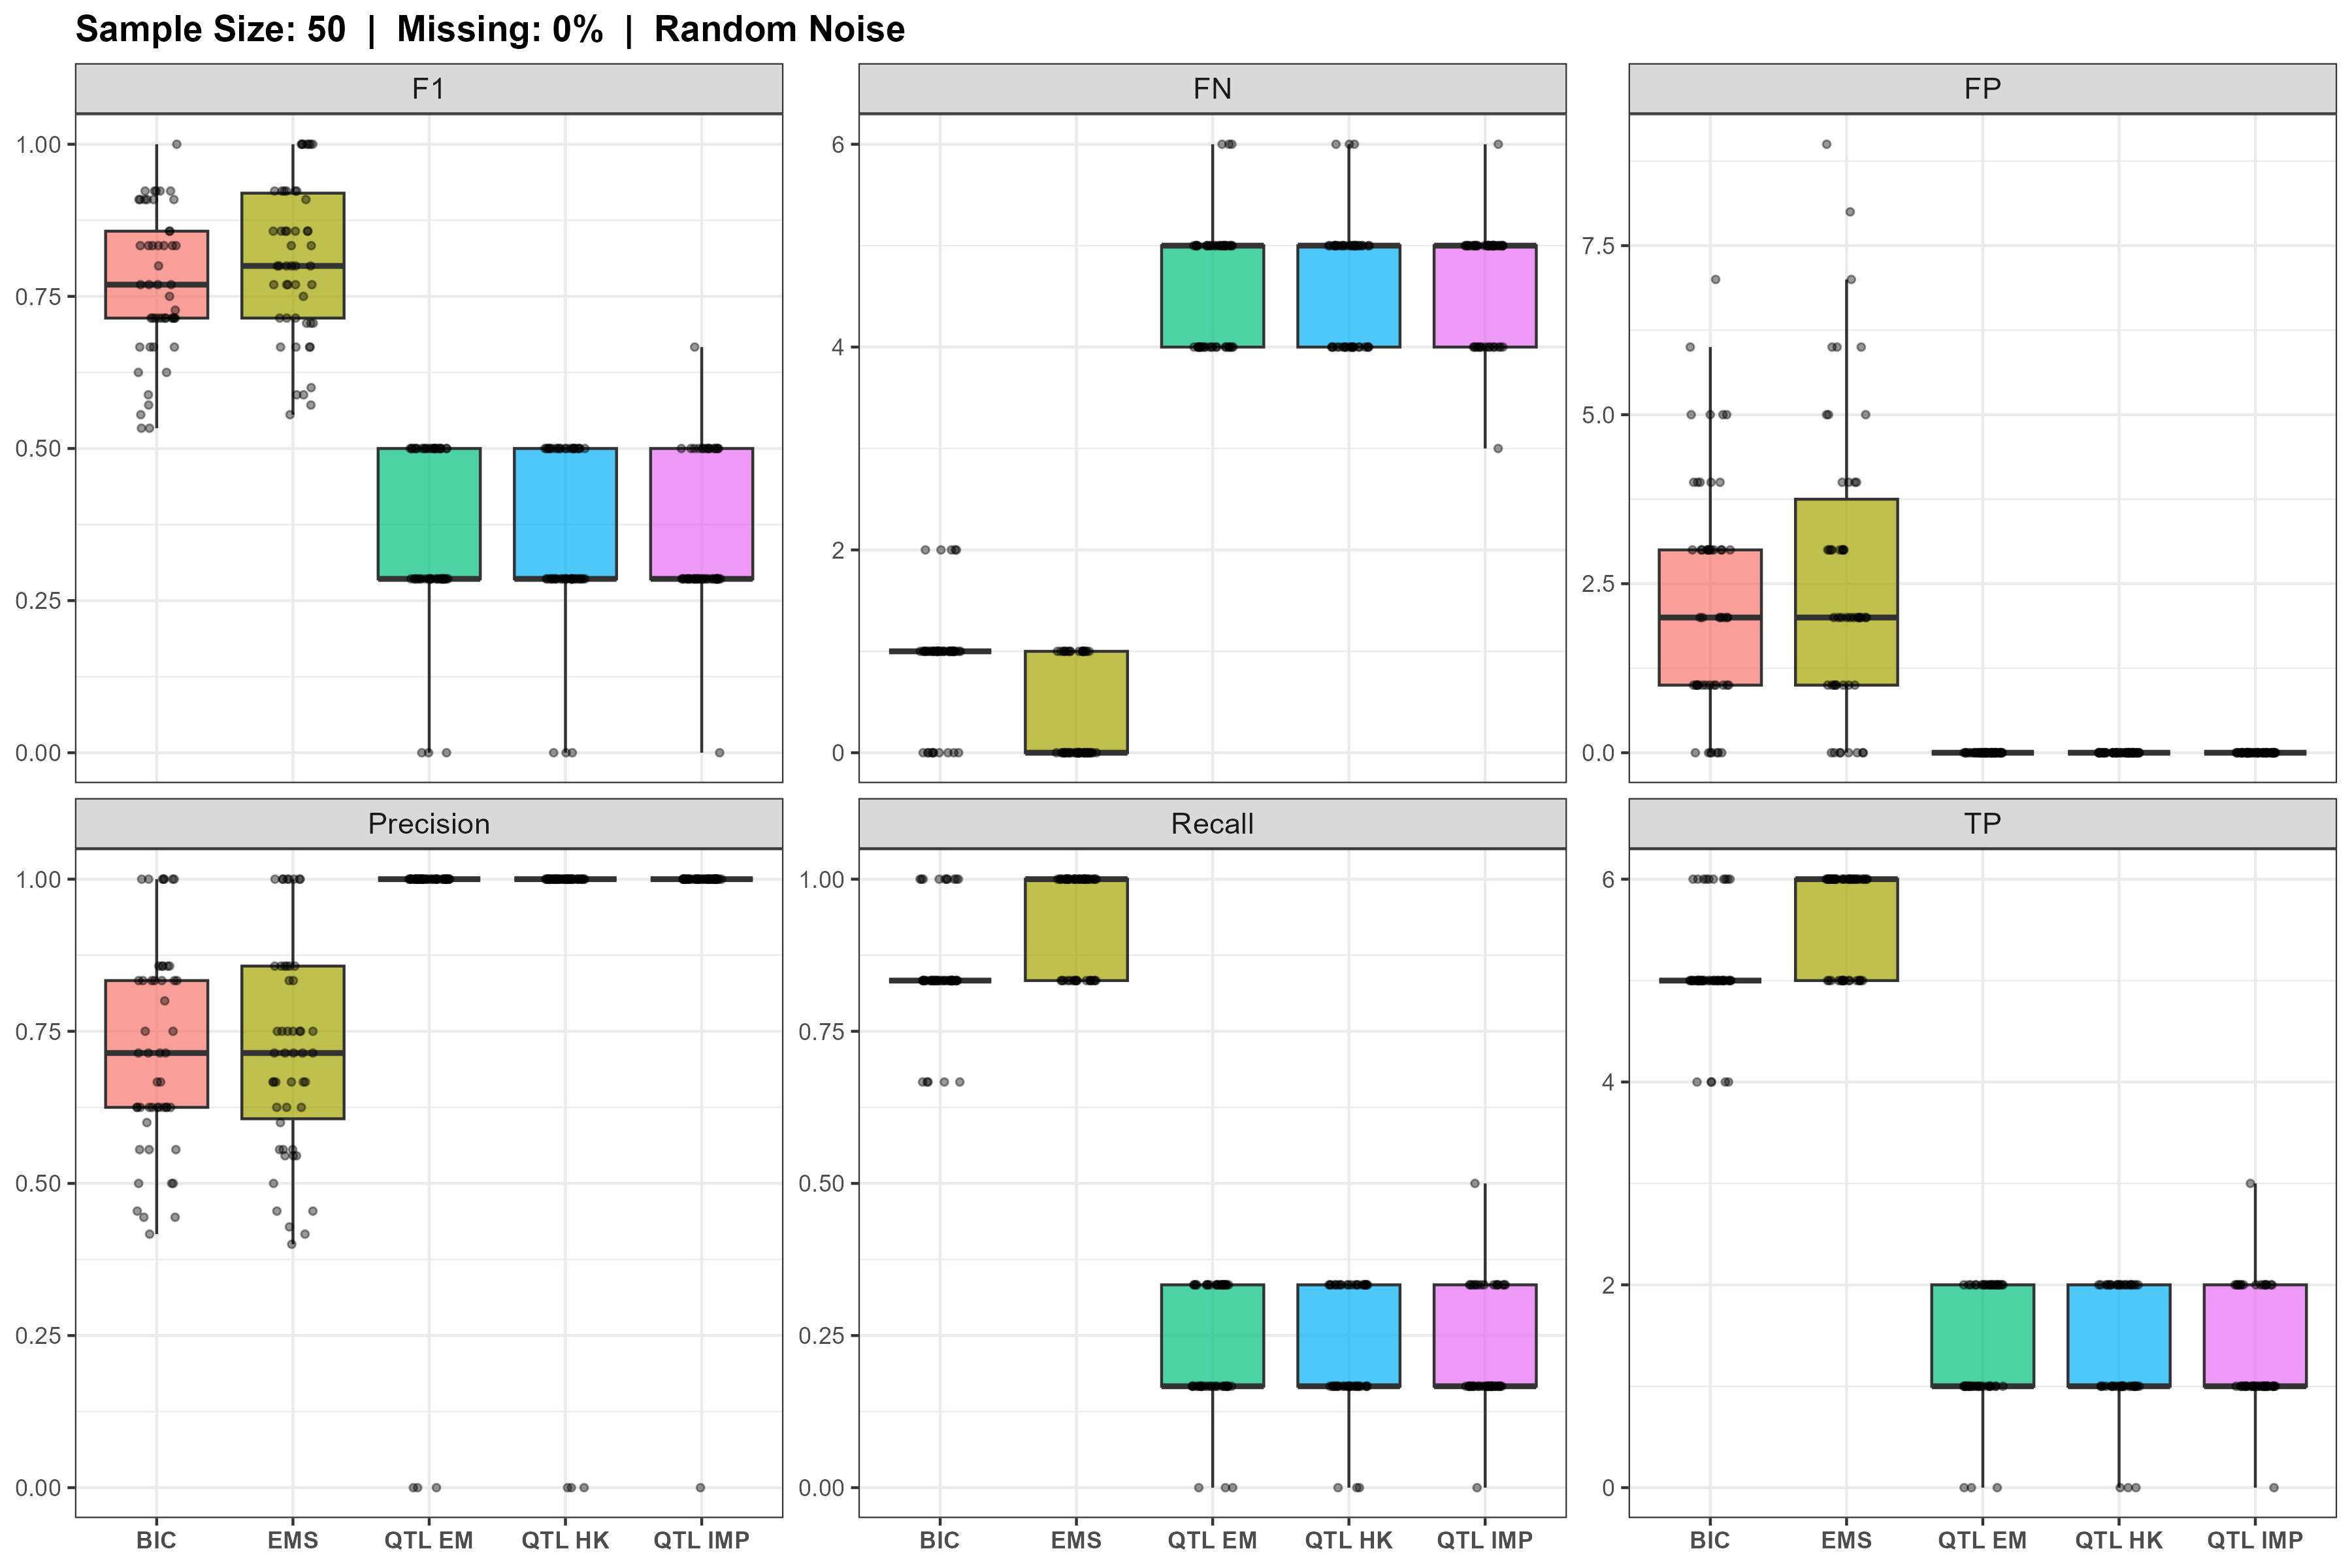
\includegraphics[width=0.95\textwidth,height=0.35\textheight,keepaspectratio]{./SuppFig_sim_n50_miss0_noise10.10.50.40.30.9.JPG}
\caption{Performance across simulation condition 17. Boxplots comparing F1, FN, FP, Precision, Recall, and TP metrics across baseline (BIC) and four alternative methods (EMS, QTL EM, QTL HK, QTL IMP) under random noise conditions with 0\% missing data (sample size: 50). Methods show remarkably consistent performance with complete data.}
\label{fig:sim17}

\vspace{0.5cm}

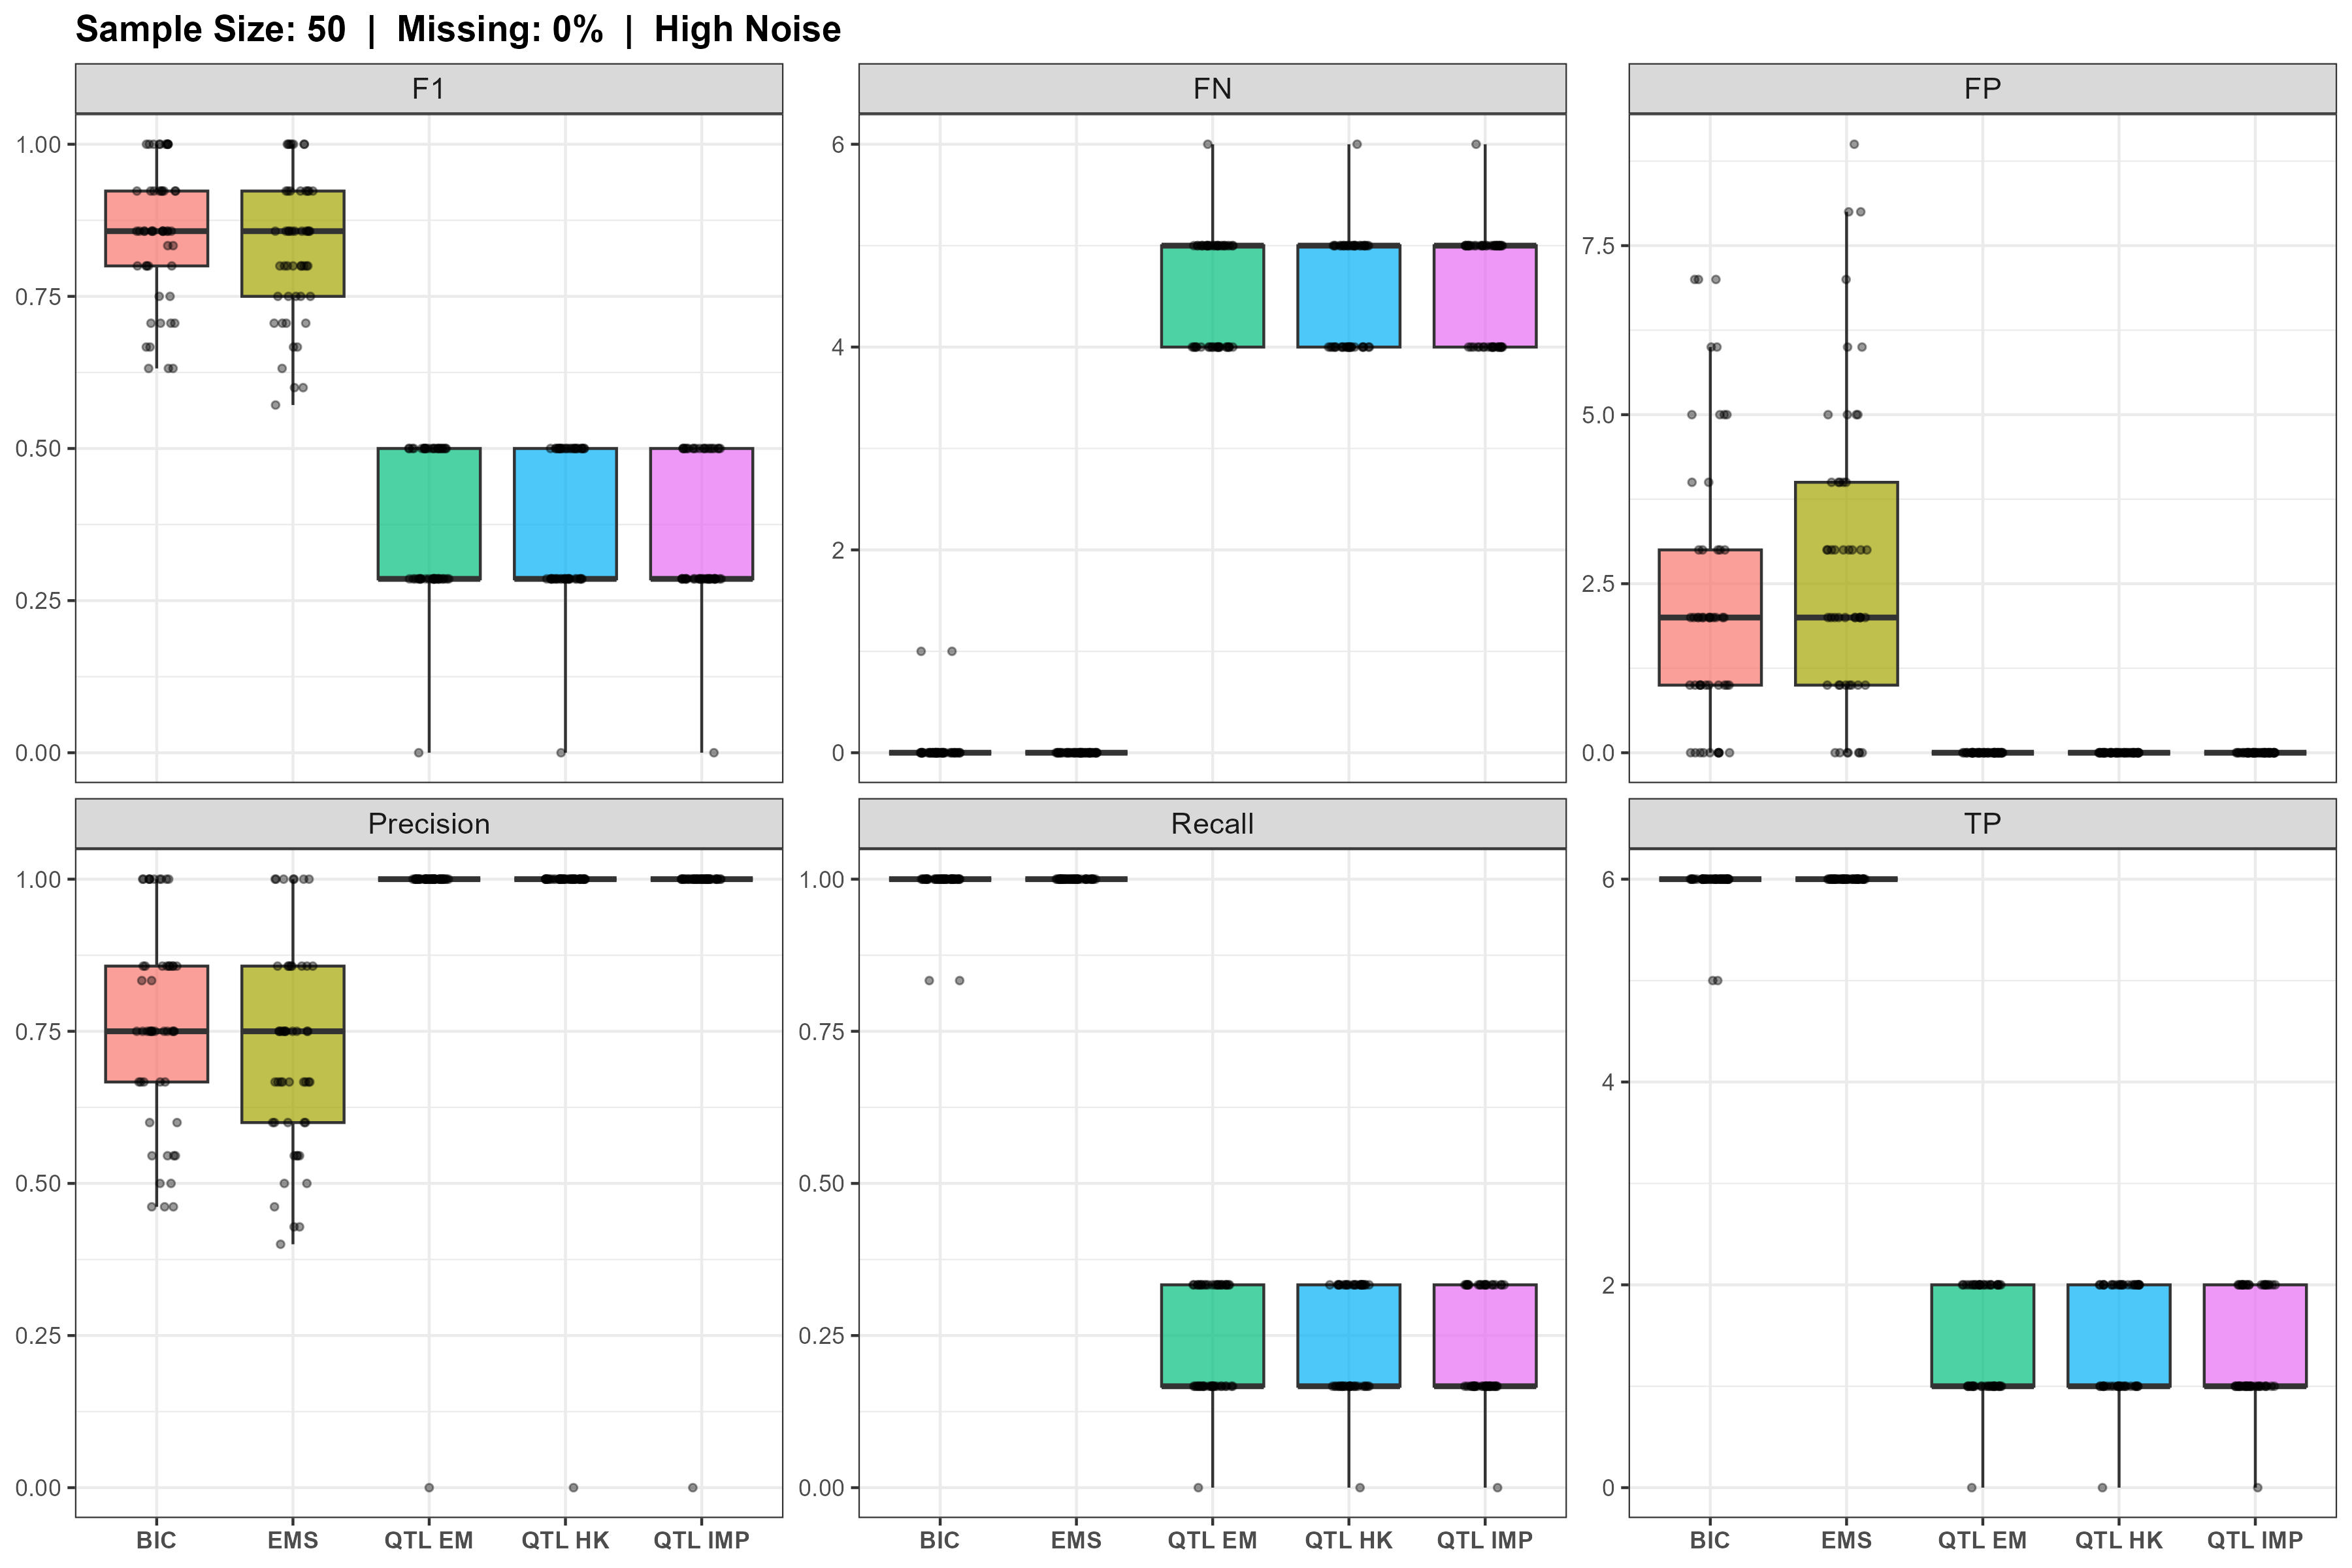
\includegraphics[width=0.95\textwidth,height=0.35\textheight,keepaspectratio]{./SuppFig_sim_n50_miss0_noise111111.JPG}
\caption{Performance across simulation condition 18. Boxplots comparing F1, FN, FP, Precision, Recall, and TP metrics across baseline (BIC) and four alternative methods (EMS, QTL EM, QTL HK, QTL IMP) under high noise conditions with 0\% missing data (sample size: 50). Despite high noise, complete data allows all methods to maintain relatively stable performance trajectories.}
\label{fig:sim18}
\end{figure}

\begin{figure}[H]
\centering
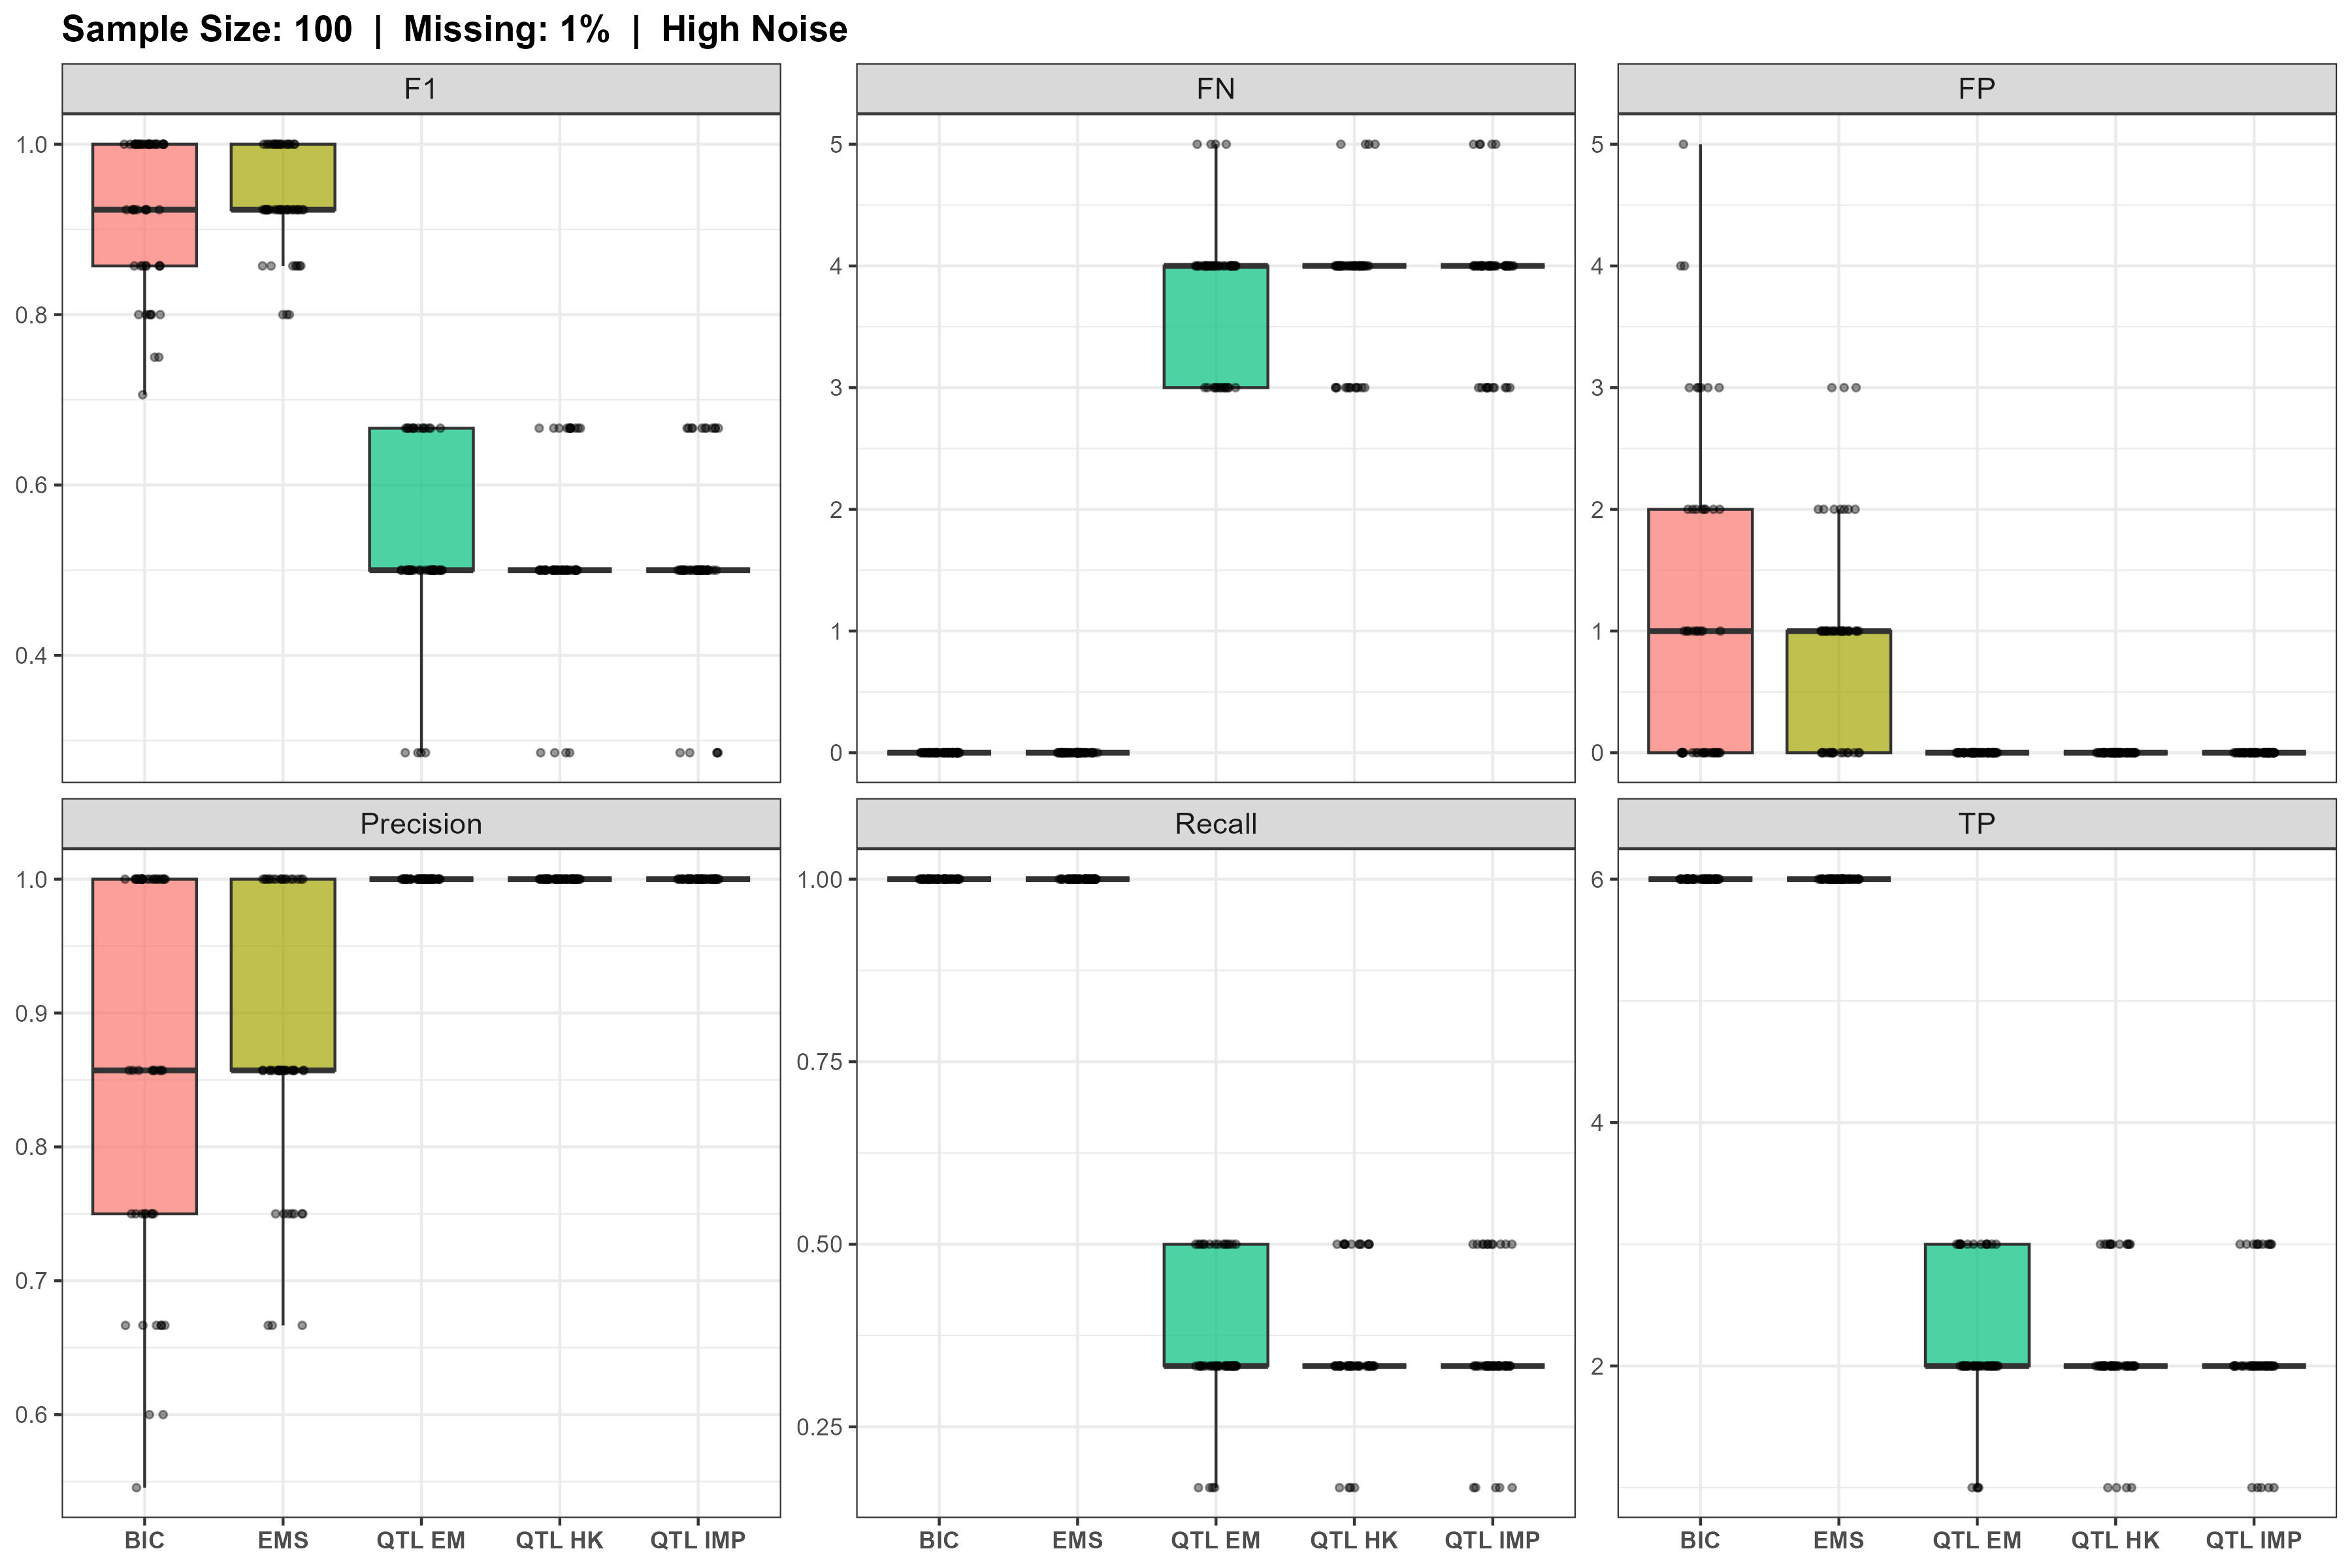
\includegraphics[width=0.95\textwidth,height=0.35\textheight,keepaspectratio]{./SuppFig_sim_n100_miss0.01_noise111111.JPG}
\caption{Performance across simulation condition 3. Boxplots comparing F1, FN, FP, Precision, Recall, and TP metrics across baseline (BIC) and four alternative methods (EMS, QTL EM, QTL HK, QTL IMP) under high noise conditions with 1\% missing data (sample size: 100). QTL HK and QTL IMP demonstrate notably improved performance over BIC and EMS in high noise scenarios.}
\label{fig:sim3}

%\vspace{0.5cm}
%
%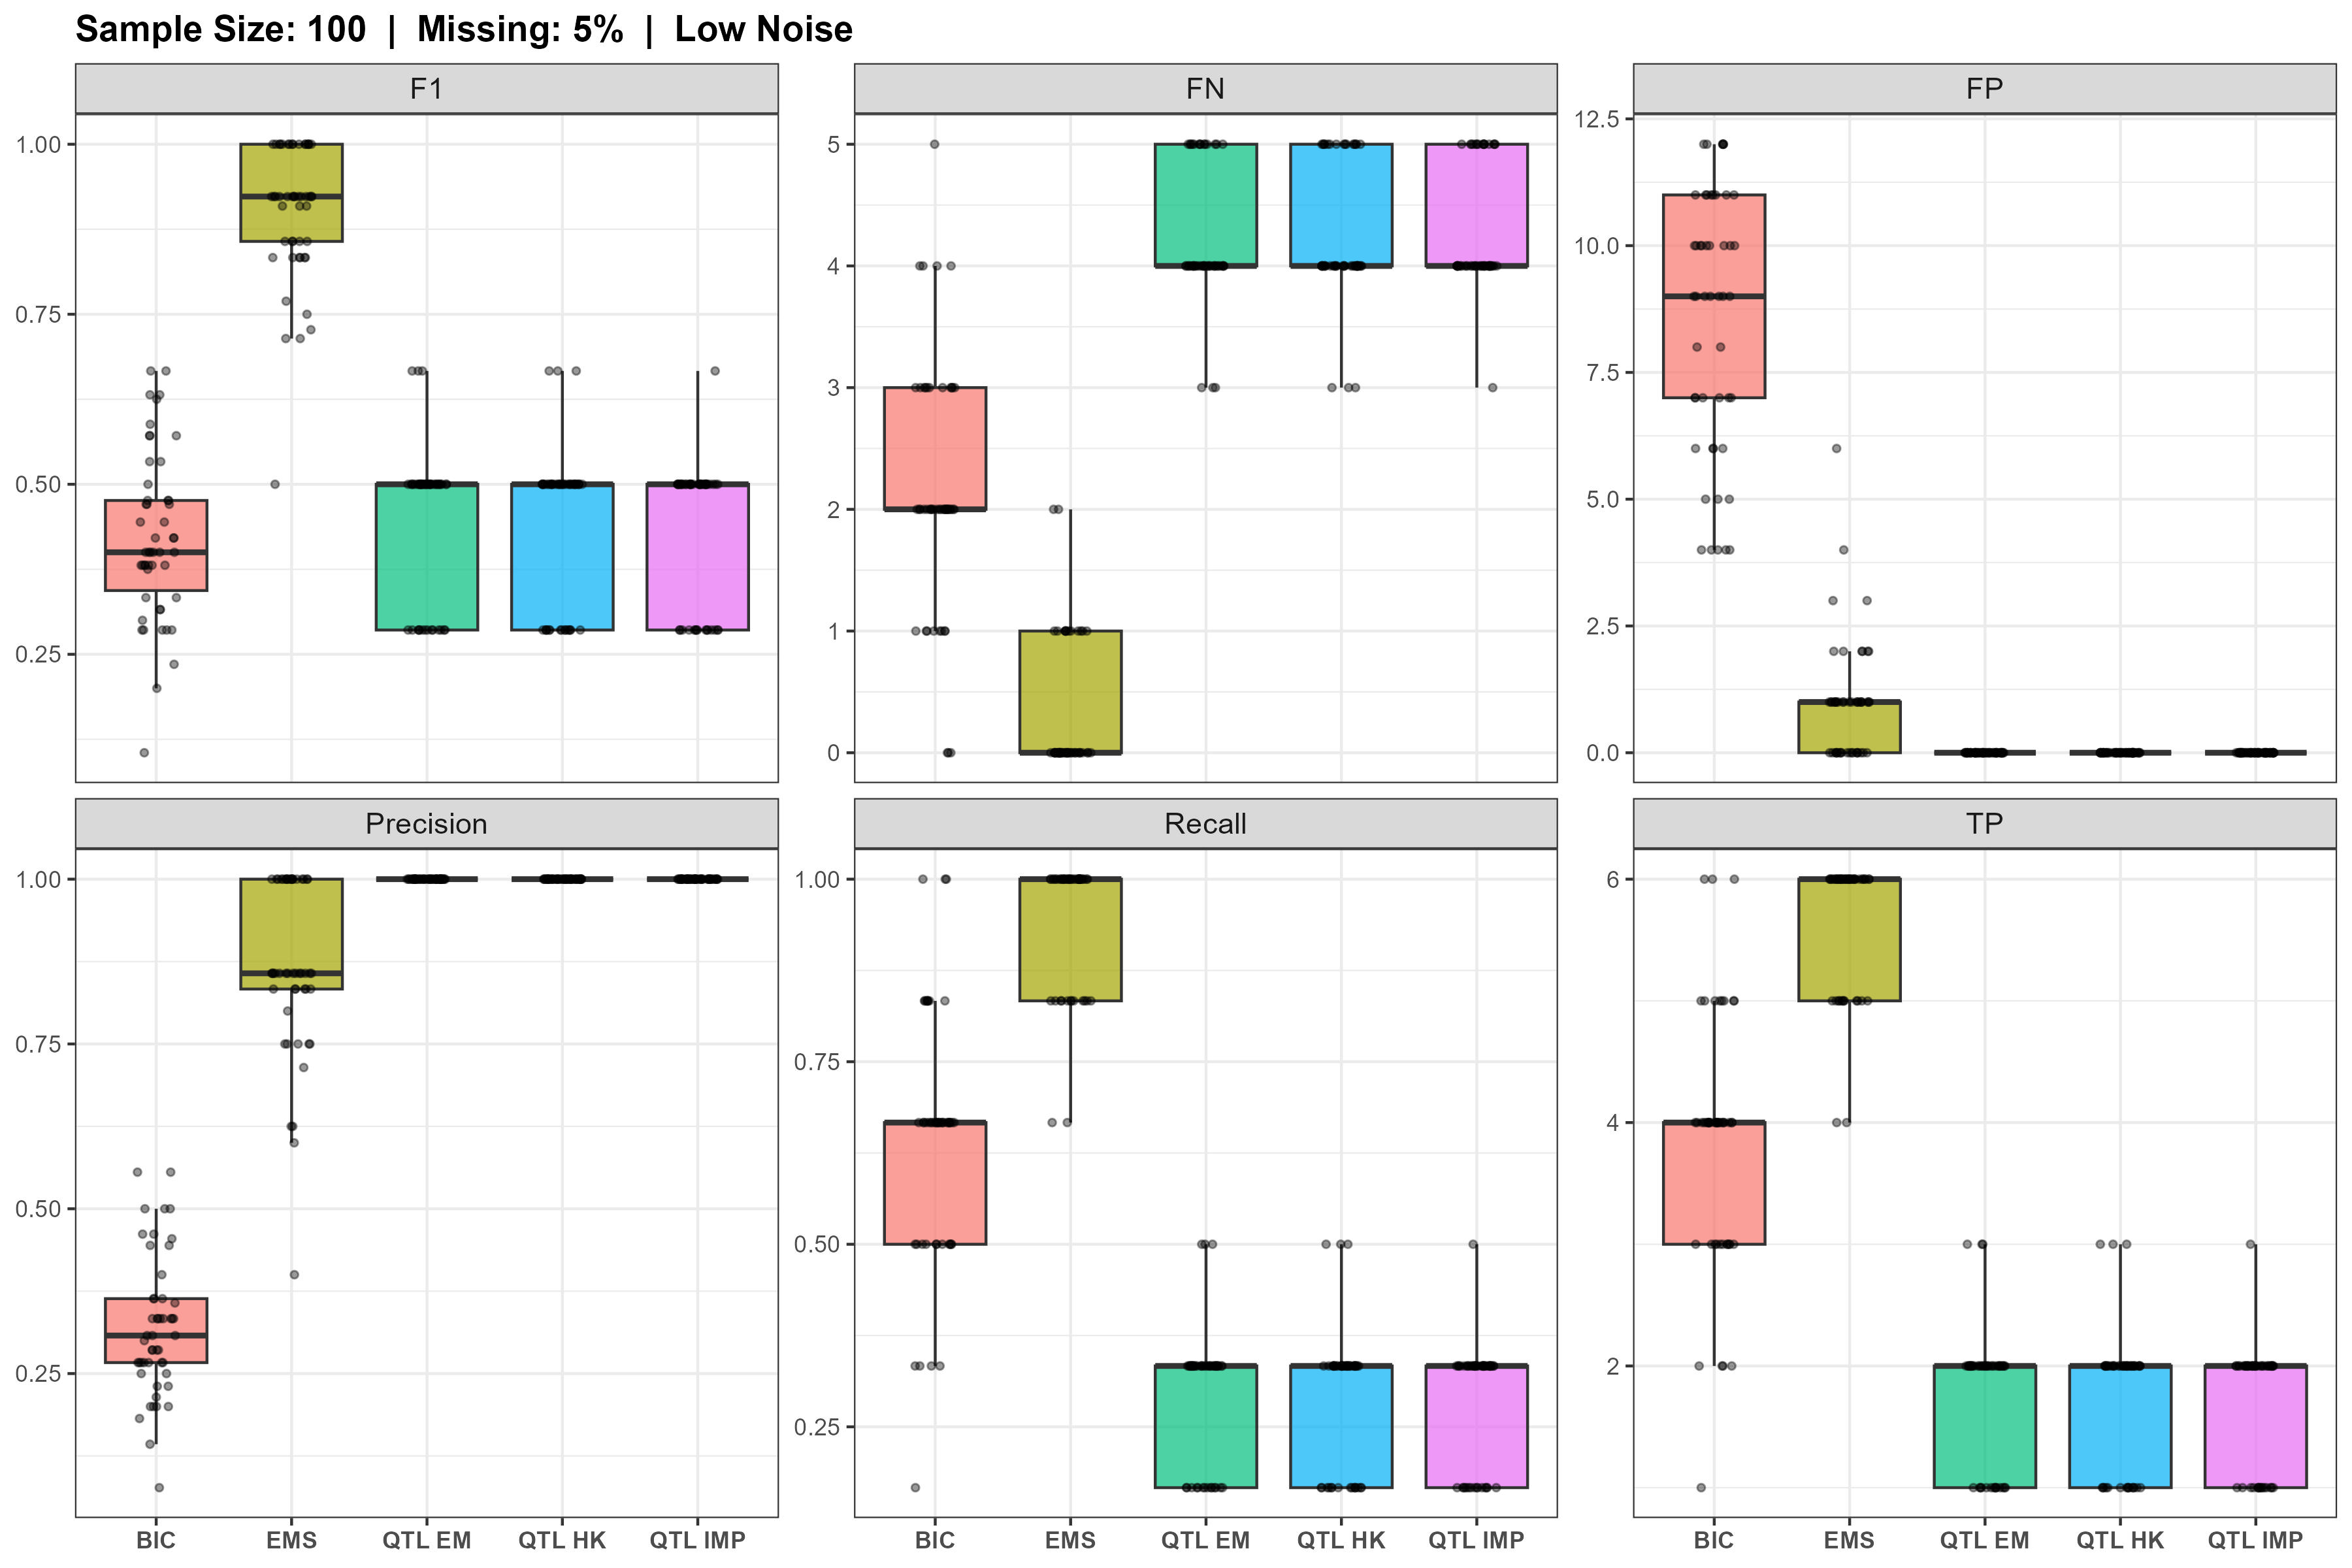
\includegraphics[width=0.95\textwidth,height=0.35\textheight,keepaspectratio]{./SuppFig_sim_n100_miss0.05_noise0.10.10.10.10.10.1.JPG}
%\caption{Performance across simulation condition 4. Boxplots comparing F1, FN, FP, Precision, Recall, and TP metrics across baseline (BIC) and four alternative methods (EMS, QTL EM, QTL HK, QTL IMP) under low noise conditions with 5\% missing data (sample size: 100).}
%\label{fig:sim4}
\end{figure}


\clearpage



\end{document}
